\section{Mức độ 7,8 điểm}
\setcounter{dang}{0}
\Opensolutionfile{ans}[ans/CD2/Muc_7_8]
\begin{dang}
	{Tìm $m$ để hàm số đạt cực trị tại $x=x_0$}
\end{dang}
\begin{ex}%[2D1K2-3]%
	[Mã 110-2017]
	Tìm giá trị thực của tham số $m$ để hàm số $y=\dfrac{1}{3}{x^3}-m{x^2}+\left(m^2-4\right)x+3$ đạt cực đại tại $x=3$.
	\choice
	{$m=-1$}
	{$m=-7$}
	{\True $m=5$}
	{$m=1$}
	\loigiai{
		Ta có $y^{\prime}=x^2-2mx+\left(m^2-4\right)$ ; $y^{\prime \prime}=2x-2m$ .\\
		Hàm số $y=\dfrac{1}{3}{x^3}-m{x^2}+\left(m^2-4\right)x+3$ đạt cực đại tại $x=3$ khi và chỉ khi: $\left\{\begin{aligned}
			&{y}'(3)=0\\ 
			&y^{\prime \prime}(3)<0\\ 
		\end{aligned}\right.$\\
		$\Leftrightarrow\left\{\begin{aligned}
			&9-6m+m^2-4=0\\ 
			&6-2m<0\\ 
		\end{aligned}\right.\Leftrightarrow\left\{\begin{aligned}
			&{m^2}-6m+5=0\\ 
			&m>3\\ 
		\end{aligned}\right.\Leftrightarrow\left\{\begin{aligned}
			&\left[\begin{aligned}
				&m=1\left( \text{loại}\right) \\ 
				&m=5\left(\text{thoả mãn}\right)\\ 
			\end{aligned}\right.\\ 
			&m>3\\ 
		\end{aligned}\right.$.\\
		Vậy $m=5$ là giá trị cần tìm.
	}
\end{ex}
\begin{ex}%[2D1K2-3]%
	[Chuyên Hạ Long 2019]
	Tìm $m$ để hàm số $y=x^3-2m{x^2}+mx+1$ đạt cực tiểu tại $x=1$.
	\choice
	{không tồn tại $m$}
	{$m=\pm 1$}
	{\True $m=1$}
	{$m\in\left\{1;2\right\}$}
	\loigiai{
		Ta có $y^{\prime} = 3x^2 -4mx + m; y^{\prime \prime} = 6x - 4m$.\\
		Hàm số đạt cực tiểu tại điểm $x=1$ $\Leftrightarrow\left\{\begin{aligned}
			&{y}'(1)=0\\ 
			&y^{\prime \prime}(1)>0\\ 
		\end{aligned}\right.\Leftrightarrow\left\{\begin{aligned}
			&3-4m+m=0\\ 
			&6-4m>0\\ 
		\end{aligned}\right.\Leftrightarrow\left\{\begin{aligned}
			&m=1\\ 
			&m<\dfrac{3}{2}\\ 
		\end{aligned}\right.\Leftrightarrow m=1.$\\
	}
\end{ex}
\begin{ex}%[2D1K2-3]
	Tìm tất cả các giá trị của tham số $m$ để hàm số $y=x^3-3x^2+mx+1$ đạt cực tiểu tại $x=2$.
	\choice
	{\True $m=0$}
	{$m>4$}
	{$0\le m<4$}
	{$0<m\le 4$}
	\loigiai{
		$y^{\prime}=3x^2-6x+m$; $y^{\prime \prime}=6x-6$.\\
		Hàm số đạt cực tiểu tại $x=2\Leftrightarrow\left\{\begin{aligned}
			&{y}'(2)=0\\ 
			&y^{\prime \prime}(2)>0\\ 
		\end{aligned}\right.\Leftrightarrow\left\{\begin{aligned}
			&m=0\\ 
			&6>0\\ 
		\end{aligned}\right.\Leftrightarrow m=0$.
	}
\end{ex}
\begin{ex}%[2D1K2-3]%[THPT An Lão Hải Phòng 2019]
	Có bao nhiêu số thực $m$ để hàm số $y=\dfrac{1}{3}{x^3}-m{x^2}+\left(m^2-m+1\right)x+1$ đạt cực đại tại $x=1$?
	\choice
	{$0$}
	{$2$}
	{\True $1$}
	{$3$}
	\loigiai{
		$y^{\prime}=x^2-2mx+m^2-m+1; y^{\prime \prime}=2x-2m$\\
		Hàm số đạt cực đại tại $x=1 \Leftrightarrow \left\{\begin{aligned}
			&y^{\prime}(1)=0\\ 
			&y^{\prime \prime}(1)<0\\ 
		\end{aligned}\right.\Leftrightarrow\left\{\begin{aligned}
			&{m^2}-3m+2=0\\ 
			&2-2m<0\\ 
		\end{aligned}\right.\Leftrightarrow\left\{\begin{aligned}
			&m=1\vee m=2\\ 
			&m>1\\ 
		\end{aligned}\right.\Leftrightarrow m=2$.
	}
\end{ex}
\begin{ex}%[2D1K2-3]%[THPT Thăng Long-Hà Nội-Lần 2-2019]
	Tìm tập hợp tất cả các giá trị của $m$ để hàm số $y=x^3+\left(3m-1\right){x^2}+m^2x-3$ đạt cực tiểu tại $x=-1$.
	\choice
	{$\left\{5;1\right\}$}
	{\True $\left\{5\right\}$}
	{$\varnothing$}
	{$\left\{1\right\}$}
	\loigiai{
		Ta có $y^{\prime}=3x^2+2\left(3m-1\right)x+m^2\Rightarrow y^{\prime \prime}=6x+6m-2$.\\
		Hàm số đạt cực tiểu tại $x=-1\Leftrightarrow\left\{\begin{aligned}
			&{f}'\left(-1\right)=0\\ 
			&{f}''\left(-1\right)>0\\ 
		\end{aligned}\right.\Leftrightarrow\left\{\begin{aligned}
			&{m^2}-6m+5=0\\ 
			& 6m-8>0\\ 
		\end{aligned}\right.\Leftrightarrow\left\{\begin{aligned}
			&\left[\begin{aligned}
				& m=1\\ 
				& m=5\\ 
			\end{aligned}\right.\\ 
			& m>\dfrac{4}{3}\\ 
		\end{aligned}\right.\\ \Leftrightarrow m=5$.
	}
\end{ex}
\begin{ex}%[2D1K2-3]%[THPT Kinh Môn-2019]
	Tìm tất cả các giá trị thực của tham số $m$ để hàm số $y=\dfrac{1}{3}{x^3}-m{x^2}+\left(m+1\right)x-1$ đạt cực đại tại $x=-2$?
	\choice
	{$m=2$}
	{$m=3$}
	{Không tồn tại $m$}
	{\True $m=-1$}
	\loigiai{
		
		Ta có $y^{\prime}=x^2-2mx+m+1; y^{\prime \prime}=2x-2m$.\\
		Hàm số đạt cực đại tại $x=-2 \Leftrightarrow \heva{& f^{\prime}(-2)=0\\ & f^{\prime \prime}(-2)<0} \Leftrightarrow \heva{& 5m + 5 = 0 \\ & -4-2m<0} \Leftrightarrow \heva{& m =-1\\& m >-2} \Leftrightarrow m = -1$.
	}
\end{ex}
\begin{ex}%[2D1K2-3]%[Chuyên ĐHSPHN-Lần 3-2019]
	Tập hợp các số thực $m$ để hàm số $y=x^3-3m{x^2}+(m+2)x-m$ đạt cực tiểu tại $x=1$ là.
	\choice
	{$\left\{1\right\}$}
	{$\left\{-1\right\}$}
	{\True $\varnothing$}
	{$\mathbb{R}$}
	\loigiai{
		$y^{\prime}=3x^2-6mx+m+2; y^{\prime \prime}=6x-6m$.\\
		Hàm số đạt cực tiểu tại $x=1 \Leftrightarrow \left\{\begin{aligned}
			&y^{\prime}(1)=0\\ 
			&y^{\prime \prime}(1)>0\\ 
		\end{aligned}\right.\Leftrightarrow\left\{\begin{aligned}
			&-5m+5=0\\ 
			&6-6m>0\\ 
		\end{aligned}\right.\Leftrightarrow\left\{\begin{aligned}
			&m=1\\ 
			&m<1.\\ 
		\end{aligned}\right.$ \\
		Vậy không có giá trị của $m$ thoả đề bài.
	}
\end{ex}
\begin{ex}%[2D1K2-3]%[Chuyên QH Huế-Lần 2-2019]
	Xác định tham số $m$ sao cho hàm số $y=x+m\sqrt{x}$ đạt cực trị tại $x=1$.
	\choice
	{\True $m=-2$}
	{$m=2$}
	{$m=-6$}
	{$m=6$}
	\loigiai{
		$y^{\prime}=f^{\prime}(x)=1+\dfrac{m}{2\sqrt{x}},\left(x>0\right)$\\
		Để hàm số đạt cực trị tại $x=1$ thì $f^{\prime}(1)=0\Leftrightarrow 1+\dfrac{m}{2}=0\Leftrightarrow m=-2$.\\
		Thử lại với $m=-2$, hàm số $y=x-2\sqrt{x}$ có cực tiểu tại $x=1$, do đó $m=-2$ thỏa mãn yêu cầu đề bài.
	}
\end{ex}
\begin{ex}%[2D1K2-3]%[Trường THPT Hoàng Hoa Thám-Hưng Yên 2019]
	Tìm tất cả tham số thực $m$ để hàm số $y=\left(m-1\right){x^4}-\left(m^2-2\right){x^2}+2019$ đạt cực tiểu tại $x=-1$.
	\choice
	{$m=0$}
	{$m=-2$}
	{$m=1$}
	{\True $m=2$}
	\loigiai{
		Tập xác định $\mathscr{D}=\mathbb{R}$.\\
		Đạo hàm $y^{\prime}=4\left(m-1\right){x^3}-2\left(m^2-2\right)x$.\\
		Hàm số đạt cực tiểu tại $x=-1$ $\Rightarrow{y}'\left(-1\right)=0$ $\Leftrightarrow-4\left(m-1\right)+2\left(m^2-2\right)=0$ $\Leftrightarrow\hoac{&m=0\\ 
			&m=2.}$
		\begin{itemize}
			\item Với $m=0$, hàm số trở thành $y=-x^4+2x^2+2019$. Dễ thấy hàm số đạt cực đại tại $x=-1$.
			\item Với $m=2$, hàm số trở thành $y=x^4-2x^2+2019$. Dễ thấy hàm số đạt cực tiểu tại $x=-1$.
		\end{itemize}
		Vậy $m=2$ thì hàm số $ y=\left(m-1\right){x^4}-\left(m^2-2\right){x^2}+2019$ đạt cực tiểu tại $ x=-1$.
	}
\end{ex}
\begin{ex}%[2D1G2-3]%[Chuyên Trần Phú Hải Phòng 2019]
	Cho hàm số $y=f(x)$ xác định trên tập số thực $\mathbb{R}$ và có đạo hàm $ f^{\prime}(x)=\left(x-\sin x\right)\left(x-m-3\right){\left(x-\sqrt{9-m^2}\right)^3},$ $\forall x\in\mathbb{R}$ ($m$ là tham số). Có bao nhiêu giá trị nguyên của $m$ để hàm số $y=f(x)$ đạt cực tiểu tại $x=0$?
	\choice
	{\True $6$}
	{$7$}
	{$5$}
	{$4$}
	\loigiai{
		Điều kiện: $9-m^2\ge 0\Leftrightarrow-3\le m\le 3$.
		\begin{itemize}
			\item \textbf{Trường hợp 1.} $0\le m<3$ ta có bảng biến thiên.\\
			\begin{center}
				
\begin{tikzpicture}
					\tkzTabInit[nocadre=false,lgt=1.2,espcl=3,deltacl=0.6]
					{$x$/0.6,$y^{\prime}$/0.6,$y$/2}
					{$-\infty$,$0$,$\sqrt{9-m^2}$,$m+3$,$+\infty$}
					\tkzTabLine{,-,0,+,0,-,0,+,}
					\tkzTabVar{+/,-/,+/,-/,+/}
				\end{tikzpicture}
			\end{center}
			\item 	\textbf{Trường hợp 2.} $-3\le m<0$ ta có bảng biến thiên.\begin{center}
				
\begin{tikzpicture}
					\tkzTabInit[nocadre=false,lgt=1.2,espcl=3,deltacl=0.6]
					{$x$/0.6,$y^{\prime}$/0.6,$y$/2}
					{$-\infty$,$0$,$m+3$,$\sqrt{9-m^2}$,$+\infty$}
					\tkzTabLine{,-,0,+,0,-,0,+,}
					\tkzTabVar{+/,-/,+/,-/,+/}
				\end{tikzpicture}
			\end{center}
			\item \textbf{Trường hợp 3.} $m=3$ ta có bảng biến thiên.\begin{center}
				
\begin{tikzpicture}
					\tkzTabInit
					[lgt=2,espcl=4] % tùy chọn
					{$x$/0.8,$y^{\prime}$/0.8, $y$/2} % cột đầu tiên
					{$-\infty$,$0$,$6$,$+\infty$} % hàng 1 cột 2
					\tkzTabLine{,-,0,-,0,+} % hàng 2 cột 2
					\tkzTabVar{+/ , R/ , -/,+/} % hàng 3 cột 2 (2 điểm đầu)
				\end{tikzpicture}
			\end{center}
		\end{itemize}
		Từ đó suy ra $-3\le m<3\Rightarrow$ có $6$ giá trị nguyên của $m$ thỏa mãn.}
\end{ex}
\begin{ex}%[2D1G2-3]%[Mã 101-2018]
	Có bao nhiêu giá trị nguyên của tham số $m$ để hàm số $y=x^8+\left(m-2\right){x^5}-\left(m^2-4\right){x^4}+1$ đạt cực tiểu tại $x=0$?
	\choice
	{Vô số}
	{$3$}
	{$5$}
	{\True $4$}
	\loigiai{
		Ta có 
		\allowdisplaybreaks
		\begin{eqnarray*}
			y&=&x^8+\left(m-2\right){x^5}-\left(m^2-4\right){x^4}+1\Rightarrow{y}'=8x^7+5\left(m-2\right){x^4}-4\left(m^2-4\right){x^3}.\\
			y^{\prime}&=&0\Leftrightarrow{x^3}\left(8x^4+5\left(m-2\right)x-4\left(m^2-4\right)\right)=0\\
			&\Leftrightarrow&\hoac{&x=0\\&g(x)=8x^4+5\left(m-2\right)x-4\left(m^2-4\right)=0.}
		\end{eqnarray*}
		Xét hàm số $ g(x)=8x^4+5\left(m-2\right)x-4\left(m^2-4\right)$ có $g'(x)=32x^3+5\left(m-2\right)$. 	Ta thấy $g'(x)=0$ có một nghiệm nên $g(x)=0$ có tối đa hai nghiệm.
		\begin{itemize}
			\item \textbf{Trường hợp 1.}  Nếu $g(x)=0$ có nghiệm $x=0$ $\Rightarrow m=2$ hoặc $m=-2$.\\
			Với $m=2$ thì $x=0$ là nghiệm bội $4$ của $g(x)$. Khi đó $x=0$ là nghiệm bội $7$ của $y^{\prime}$ và $y^{\prime}$ đổi dấu từ âm sang dương khi đi qua điểm $x=0$ nên $x=0$ là điểm cực tiểu của hàm số. Vậy $m=2$ thỏa ycbt.\\
			Với $m=-2$ thì $g(x)=8x^4-20x=0\Leftrightarrow\hoac{
				&x=0\\ 
				&x=\sqrt[3]{\dfrac{5}{2}}.}$\\
			Bảng biến thiên
			\begin{center}
				
\begin{tikzpicture}
					\tkzTabInit
					[lgt=2,espcl=4] % tùy chọn
					{$x$/1.2,$y^{\prime}$/0.8, $y$/2} % cột đầu tiên
					{$-\infty$,$0$,$\sqrt[3]{\dfrac{5}{2}}$,$+\infty$} % hàng 1 cột 2
					\tkzTabLine{,-,0,-,0,+} % hàng 2 cột 2
					\tkzTabVar{+/ , R/ , -/,+/} % hàng 3 cột 2 (2 điểm đầu)
				\end{tikzpicture}
			\end{center}
			Dựa vào bảng biến thiên $x=0$ không là điểm cực tiểu của hàm số. Vậy $m=-2$ không thỏa yêu cầu bài toán.
			\item \textbf{Trường hợp 2.} $g(0)\ne 0$ $\Leftrightarrow m\ne\pm 2$. \\Để hàm số đạt cực tiểu tại $x=0\Leftrightarrow g(0)>0$ $\Leftrightarrow{m^2}-4<0\Leftrightarrow-2<m<2$. 	Do $m\in\mathbb{Z}$ nên $m\in\left\{-1;0;1\right\}$.		\end{itemize}
		Vậy cả hai trường hợp ta được $4$ giá trị nguyên của $m$ thỏa yêu cầu bài toán.
	}
\end{ex}
\begin{ex}%[2D1G2-3]%[Chuyên Quang Trung-Bình Phước 2019]
	Tất cả các giá trị thực của tham số $m$ để hàm số $y=\dfrac{x^5}{5}-\dfrac{m{x^4}}{4}+2$ đạt cực đại tại $x=0$ là
	\choice
	{$m\in\mathbb{R}$}
	{$m<0$}
	{Không tồn tại $m$}
	{\True $m>0$}
	\loigiai{
		Đặt $f(x)=\dfrac{x^5}{5}-\dfrac{m{x^4}}{4}+2$. Ta có $f^{\prime}(x)=x^4-m{x^3}$.
		\begin{itemize}
			\item Khi $m=0$ thì $f^{\prime}(x)=x^4\ge 0$, $\forall x\in\mathbb{R}$ nên hàm số không có cực trị.
			\item 	Khi $m\ne 0$, xét $f^{\prime}(x)=0\Leftrightarrow{x^4}-m{x^3}=0\Leftrightarrow{x^3}\left(x-m\right)=0\Leftrightarrow\hoac{&x=0\\ 
				&x=m.}$		
			\begin{itemize}
				\item \textbf{Trường hợp 1.} $m>0$ ta có bảng biến thiên:
				\begin{center}
					\begin{tikzpicture}
						\tkzTabInit[nocadre=false,lgt=1.2,espcl=2.5,deltacl=0.6]
						{$x$/0.6,$f^{\prime}(x)$/0.6,$f(x)$/2}
						{$-\infty$,$0$,$m$,$+\infty$}
						\tkzTabLine{,+,0,-,0,+,}
						\tkzTabVar{-/$-\infty$,+/$2$,-/$f(m)$,+/$+\infty$}
					\end{tikzpicture}
				\end{center}
				Dựa vào bảng biến thiên ta thấy hàm số đạt cực đại tại $x=0$.
				\item \textbf{Trường hợp 2.} $m<0$ ta có bảng biến thiên:
				\begin{center}
					\begin{tikzpicture}
						\tkzTabInit[nocadre=false,lgt=1.2,espcl=2.5,deltacl=0.6]
						{$x$/0.6,$f^{\prime}(x)$/0.6,$f(x)$/2}
						{$-\infty$,$m$,$0$,$+\infty$}
						\tkzTabLine{,+,0,-,0,+,}
						\tkzTabVar{-/$-\infty$,+/$f(m)$,-/$2$,+/$+\infty$}
					\end{tikzpicture}
				\end{center}
				Dựa vào bảng biến thiên ta thấy hàm số đạt cực tiểu tại $x=0$.
			\end{itemize}
		\end{itemize}
		Như vậy, để hàm số đạt cực đại tại $x=0$ thì $m>0$.
	}
\end{ex}
\begin{ex}%[2D1G2-3]
	Có bao nhiêu giá trị nguyên của $m$ thuộc khoảng $\left(-2019;2019\right)$ để hàm số $y=\dfrac{m-1}{5}{x^5}+\dfrac{m+2}{4}{x^4}+m+5$ đạt cực đại tại $x=0$?
	\choice
	{$101$}
	{\True $2016$}
	{$100$}
	{$10$}
	\loigiai{
		Ta xét $m=1\Rightarrow y=\dfrac{3}{4}{x^4}+6\Rightarrow{y}'=3x^3\Rightarrow{y}'=0\Rightarrow x=0$.\\
		Ta có bảng xét dấu $y^{\prime}=2x^3$.
		\begin{center}
			\begin{tikzpicture}
				\tkzTabInit[nocadre=false,lgt=1.2,espcl=2.5,deltacl=0.6]
				{$x$/0.6,$f^{\prime}(x)$/0.6}
				{$-\infty$,$0$,$+\infty$}
				\tkzTabLine{,-,0,+,}
			\end{tikzpicture}
		\end{center}
		Dựa vào bảng xét dấu ta thấy $x=0$ là điểm cực tiểu. Suy ra $m=1$ (loại).\\
		Ta xét $m\ne 1\Rightarrow{y}'=\left(m-1\right){x^4}+\left(m+2\right){x^3}\Rightarrow y^{\prime}=0\Rightarrow\hoac{&{x_1}=0\\ 
			&{x_2}=-\dfrac{m+2}{m-1}.}$
		\begin{itemize}
			\item	\textbf{Trường hợp 1.} Xét $m>1$, suy ra $x_2<x_1$. Ta có bảng xét dấu $y^{\prime}=\left(m-1\right){x^4}+\left(m+2\right){x^3}$.
			\begin{center}
				
\begin{tikzpicture}
					\tkzTabInit[nocadre=false,lgt=1.2,espcl=2.5,deltacl=0.6]
					{$x$/1.2,$y^{\prime}$/0.6}
					{$-\infty$,$-\dfrac{m+2}{m-1}$,$0$,$+\infty$}
					\tkzTabLine{,+,0,-,0,+,}
				\end{tikzpicture}
			\end{center}
			Dựa vào bảng xét dấu ta thấy $x=0$ là điểm cực tiểu. Suy ra $m>1$ (loại).
			\item \textbf{Trường hợp 2.} $-2<m<1$, suy ra $x_2>x_1$ . Ta có bảng xét dấu $y^{\prime}=\left(m-1\right){x^4}+\left(m+2\right){x^3}$.
			\begin{center}
				
\begin{tikzpicture}
					\tkzTabInit[nocadre=false,lgt=1.2,espcl=2.5,deltacl=0.6]
					{$x$/1.2,$y^{\prime}$/0.6}
					{$-\infty$,$0$,$-\dfrac{m+2}{m-1}$,$+\infty$}
					\tkzTabLine{,-,0,+,0,-,}
				\end{tikzpicture}
			\end{center}
			Dựa, vào bảng xét dấu ta thấy $x=0$ là điểm cực tiểu. Suy ra $-2<m<1$ (loại).
			\item \textbf{Trường hợp 3.} $m<-2$, suy ra $x_2<x_1$ . Ta có bảng xét dấu $y^{\prime}=\left(m-1\right){x^4}+\left(m+2\right){x^3}$.
			\begin{center}
				
\begin{tikzpicture}
					\tkzTabInit[nocadre=false,lgt=1.2,espcl=2.5,deltacl=0.6]
					{$x$/1.2,$y^{\prime}$/0.6}
					{$-\infty$,$-\dfrac{m+2}{m-1}$,$0$,$+\infty$}
					\tkzTabLine{,-,0,+,0,-,}
				\end{tikzpicture}
			\end{center}
			Dựa vào bảng xét dấu ta thấy $x=0$ là điểm cực đại. Suy ra $m<-2$ (nhận).
		\end{itemize}
		Vậy tập hợp tất cả các giá trị của tham số $m$ thỏa mãn đề bài là $m<-2$. Mà $m$ thuộc khoảng $\left(-2019;2019\right)$, suy ra số giá trị nguyên của $m$ là $2016$.
	}
\end{ex}
\begin{ex}%[2D1G2-3]%[Mã 104-2018]
	Có bao nhiêu giá trị nguyên của tham số $m$ để hàm số $y=x^8+\left(m-3\right){x^5}-\left(m^2-9\right){x^4}+1$ đạt cực tiểu tại $x=0$?
	\choice
	{\True $6$}
	{Vô số}
	{$4$}
	{$7$}
	\loigiai{
		Ta có 
		\allowdisplaybreaks
		\begin{eqnarray*}
			y&=&x^8+\left(m-3\right){x^5}-\left(m^2-9\right){x^4}+1\Rightarrow{y}'=8x^7+5\left(m-3\right){x^4}-4\left(m^2-9\right){x^3}.\\
			y^{\prime}&=&0\Leftrightarrow{x^3}\left(8x^4+5\left(m-3\right)x-4\left(m^2-9\right)\right)=0.\\
			&\Leftrightarrow&\hoac{&x=0\\&g(x)=8x^4+5\left(m-3\right)x-4\left(m^2-9\right)=0.}
		\end{eqnarray*}
		Xét hàm số $g(x)=8x^4+5\left(m-3\right)x-4\left(m^2-9\right)$ có $g'(x)=32x^3+5\left(m-3\right)$.\\
		Ta thấy $g'(x)=0$ có một nghiệm nên $ g(x)=0$ có tối đa hai nghiệm.
		\begin{itemize}
			\item \textbf{Trường hợp 1.} Nếu $g(x)=0$ có nghiệm $x=0$ $\Rightarrow m=3$ hoặc $m=-3$.\\
			Với $m=3$ thì $x=0$ là nghiệm bội $4$ của $g(x)$. Khi đó $x=0$ là nghiệm bội $7$ của $y^{\prime}$ và $y^{\prime}$ đổi dấu từ âm sang dương khi đi qua điểm $x=0$ nên $x=0$ là điểm cực tiểu của hàm số. Vậy $m=3$ thỏa ycbt.\\
			Với $m=-3$ thì $g(x)=8x^4-30x=0\Leftrightarrow\hoac{	&x=0\\ 
				&x=\sqrt[3]{\dfrac{15}{4}}.}$\\
			Bảng biến thiên
			\begin{center}
				
\begin{tikzpicture}
					\tkzTabInit
					[lgt=2,espcl=4] % tùy chọn
					{$x$/1.2,$y^{\prime}$/0.8, $y$/2} % cột đầu tiên
					{$-\infty$,$0$,$\sqrt[3]{\dfrac{15}{4}}$,$+\infty$} % hàng 1 cột 2
					\tkzTabLine{,-,0,-,0,+} % hàng 2 cột 2
					\tkzTabVar{+/$+\infty$ , R/ , -/,+/$+\infty$} % hàng 3 cột 2 (2 điểm đầu)
				\end{tikzpicture}
			\end{center}
			Dựa vào bảng biến thiên $x=0$ không là điểm cực tiểu của hàm số. Vậy $ m=-3$ không thỏa ycbt.
			\item \textbf{Trường hợp 2.} $g(0)\ne 0$ $\Leftrightarrow m\ne\pm 3$. Để hàm số đạt cực tiểu tại $x=0$ $\Leftrightarrow g(0)>0$ $\Leftrightarrow{m^2}-9<0\Leftrightarrow-3<m<3$. 		Do $m\in\mathbb{Z}$ nên $ m\in\left\{-2;-1;0;1;2\right\}$.
		\end{itemize}
		Vậy cả hai trường hợp ta được $6$ giá trị nguyên của $m$ thỏa yêu cầu bài toán.
	}
\end{ex}
\begin{ex}%[2D1G2-3]%[Mã 103-2018] 
	Có bao nhiêu giá trị nguyên của tham số $ m$ để hàm số $y=x^8+\left(m-4\right){x^5}-\left(m^2-16\right){x^4}+1$ đạt cực tiểu tại $x=0$.
	\choice
	{\True $8$}
	{Vô số}
	{$7$}
	{$9$}
	\loigiai{
		Ta có $y^{\prime}=8x^7+5\left(m-5\right){x^4}-4\left(m^2-16\right){x^3}x^3\left[8x^4+5\left(m-4\right)x-4\left(m^2-16\right)\right]=x^3\cdot g(x)$.\\
		Với $g(x)=8x^4+5\left(m-5\right)x-4\left(m^2-16\right)$.
		\begin{itemize}
			\item\textbf{Trường hợp 1.} $g(0)=0\Leftrightarrow m=\pm 4$.
			\begin{itemize}
				\item Với $m=4\Rightarrow y^{\prime}=8x^7$. Suy ra $x=0$ là điểm cực tiểu của hàm số.
				\item Với $m=-4\Rightarrow y^{\prime}=8x^4\left(x^3-5\right)$. Suy ra $x=0$ không là điểm cực trị của hàm số.
			\end{itemize}
			\item \textbf{Trường hợp 2.} $g(0)\ne 0\Leftrightarrow m\ne\pm 4$.\\
			Để hàm số đạt cực tiểu tại $x=0$ thì qua giá trị $x=0$ dấu của $y^{\prime}$ phải chuyển từ âm sang dương do đó $g(0)>0\Leftrightarrow-4<m<4$.
		\end{itemize}
		Kết hợp hai trường hợp ta được $-4<m\le 4$.		Do $m\in\mathbb{Z}\Rightarrow m\in\left\{-3;-2;-1;0;1;2;3;4\right\}$.\\
		Vậy có $8$ giá trị nguyên của tham số $m$ thỏa mãn.
	}
\end{ex}

\begin{ex}%[2D1G2-3]
	Có bao nhiêu giá trị nguyên của tham số $m$ để hàm số $y=x^{12}+(m-5){x^7}+(m^2-25){x^6}+1$ đạt cực đại tại $x=0$?
	\choice
	{$8$}
	{\True $9$}
	{Vô số}
	{$10$}
	\loigiai{
		Ta có $y^{\prime}=12x^{11}+7(m-5){x^6}+6(m^2-25){x^5}$.
		\begin{itemize}
			\item \textbf{Trường hợp 1.} $m=5\Rightarrow y^{\prime}=12x^{11}$. \\Khi đó $y^{\prime}=0\Leftrightarrow x=0$ là nghiệm bội lẻ, đồng thời dấu của $y$ đổi từ âm sang dương, nên $x=0$ là điểm cực tiểu của hàm số,do đó không thỏa mãn, $m=5$ (loại).
			\item \textbf{Trường hợp 2.} $m=-5\Rightarrow y^{\prime}=x^6(12x^5-70)=0\Rightarrow x=0$ là nghiệm bội chẵn, do đó $y$ không đổi dấu khi đi qua $x=0$, $m=-5$ (loại).
			\item \textbf{Trường hợp 3.} $m\ne\pm 5\Rightarrow y^{\prime}=x^5\left[12x^6+7(m-5)x+6(m^2-25)\right]=x^5.g(x)$.\\
			Với $g(x)=12x^6+7(m-5)x+6(m^2-25)$, ta thấy $x=0$ không là nghiệm của $g(x)$.\\
			Để hàm số đạt cực đại tại $x=0$ thì $y’$ phải đổi dấu từ dương sang âm khi đi qua $x=0$, xảy ra khi và chỉ khi $\heva{&\mathop {\lim \limits{n \to +\infty}}\limits_{x\to {0^-}}g(x)<0\\ 
				&\mathop {\lim \limits{n \to +\infty}}\limits_{x\to {0^+}}g(x)<0}\Leftrightarrow 6(m^2-25)<0\Leftrightarrow-5<m<5.$
		\end{itemize}
		Vì $m$ nguyên nên $m=\left\{-4;-3;...;3;4\right\}$, vậy có $9$ giá trị của $m$ thỏa mãn bài toán.
	}
\end{ex}
\begin{ex}%[2D1G2-3]
	Cho hàm số $y=x^6+\left(4+m\right){x^5}+\left(16-m^2\right){x^4}+2$. Gọi $ S$ là tập hợp các gia trị $ m$ nguyên dương để hàm số đã cho đạt cực tiểu tại $x=0$. Tổng các phần tử của $S$ bằng
	\choice
	{$10$}
	{$9$}
	{\True $6$}
	{$3$}
	\loigiai{
		Ta có 
		\allowdisplaybreaks
		\begin{eqnarray*}
			y^{\prime}&=&6x^5+5\left(4+m\right){x^4}+4\left(16-m^2\right){x^3}=x^3\left(6x^2+5\left(4+m\right)x+16-m^2\right).\\
			y^{\prime}&=&0\Leftrightarrow \heva{&{x^3}=0\\ 
				&6x^2+5\left(4+m\right)x+16-m^2=0\quad (*).}\\
		\end{eqnarray*}
		$(*)$ có $\Delta=\left(4+m\right)\left(49m+4\right)$.\\
		Với mọi $m$ nguyên dương thì $\heva{
			&\Delta >0\\ 
			&\dfrac{-5\left(4+m\right)}{6}<0}$ do đó ta xét các trường hợp sau:
		\begin{itemize}
			\item \textbf{Trường hợp 1.} $16-m^2>0\Leftrightarrow 0<m<4$: $(*)$ có hai nghiệm âm phân biệt $x_1,$ $x_2,$ $\left(x_1<x_2\right)$, ta có bảng xét dấu $y^{\prime}$ như sau:
			\begin{center}
				
\begin{tikzpicture}
					\tkzTabInit[nocadre=false,lgt=1.2,espcl=2.5,deltacl=0.6]
					{$x$/0.6,$y^{\prime}$/0.6}
					{$-\infty$,$x_1$,$x_2$,$0$,$+\infty$}
					\tkzTabLine{,-,0,+,0,-,0,+,}
				\end{tikzpicture}
			\end{center}
			Lúc này $x=0$ là điểm cực tiểu.
			\item \textbf{Trường hợp 2.} $16-m^2<0\Leftrightarrow m>4$: $(*)$ có hai nghiệm trái dấu $x_1,$ $x_2,$ $\left(x_1<0<x_2\right)$, ta có bảng xét dấu $y^{\prime}$ như sau:\begin{center}
				
\begin{tikzpicture}
					\tkzTabInit[nocadre=false,lgt=1.2,espcl=2.5,deltacl=0.6]
					{$x$/0.6,$y^{\prime}$/0.6}
					{$-\infty$,$x_1$,$0$,$x_2$,$+\infty$}
					\tkzTabLine{,-,0,+,0,-,0,+,}
				\end{tikzpicture}
			\end{center}
			Từ đây suy ra $x=0$ là điểm cực đại (không thỏa mãn).
			\item \textbf{Trường hợp 3.} $(*)$ có một nghiệm bằng $0$ và một nghiệm âm, lúc này $x=0$ là nghiệm bội $4$ của đạo hàm nên không phải là điểm cực trị.
		\end{itemize}
		Vậy có ba giá trị nguyên dương của $m$ thỏa mãn yêu cầu bài toán là $1$, $2$, $3$. Tổng các phần tử của $S$ bằng $6$.
	}
\end{ex}

\begin{ex}%[2D1G2-3]%[Mã 102-2018]
	Có bao nhiêu giá trị nguyên của tham số $m$ để hàm số $ y=x^8+(m-1){x^5}-(m^2-1){x^4}+1$ đạt cực tiểu tại $x=0$?
	\choice
	{$3$}
	{\True $2$}
	{Vô số}
	{$1$}
	\loigiai{
		Ta có
		\allowdisplaybreaks
		\begin{eqnarray*} 
			y^{\prime}&=&8x^7+5(m-1){x^4}-4(m^2-1){x^3}+1=x^3\left(8x^4+5\left(m-1\right)x-4\left(m^2-1\right)\right)\\
			y^{\prime}&=&0\Leftrightarrow\hoac{&x=0\\&8x^4+5\left(m-1\right)x-4\left(m^2-1\right)=0\quad (1).}		\end{eqnarray*}
		\begin{itemize}
			\item Nếu $m=1$ thì $y^{\prime}=8x^7$, suy ra hàm số đạt cực tiểu tại $x=0$.
			\item Nếu $m=-1$ thì $y^{\prime}=0\Leftrightarrow\hoac{&x=0\\ 
				&8x^4-10x=0}\Leftrightarrow\hoac{&x=0\\ 
				&x=\sqrt[3]{\dfrac{5}{4}}}$, nhưng $x=0$ là nghiệm bội chẵn nên không phải cực trị.\\
			\item  Nếu $m\ne\pm 1$: khi đó $x=0$ là nghiệm bội lẻ. Xét  $g(x)=8x^4+5\left(m-1\right)x-4\left(m^2-1\right)$. \\Để $x=0$ là điểm cực tiểu thì $\mathop {\lim \limits{n \to +\infty}}\limits_{x\to {0^-}}g(x)=-4(m^2-1)>0\Leftrightarrow{m^2}-1<0\Leftrightarrow-1<m<1$. \\Vì $m$ nguyên nên chỉ có giá trị $m=0$.
		\end{itemize}
		Vậy chỉ có hai tham số $m$ nguyên để hàm số đạt cực tiểu tại $x=0$ là $m=0$ và $ m=1$.
	}
\end{ex}
\begin{dang}
	{Tìm $m$ để hàm số có $n$ cực trị}
\end{dang}
\begin{ex}%[2D1B2-4]
	Biết rằng hàm số $y=\left(x+a\right)^3+\left(x+b\right)^3-x^3$ có hai điểm cực trị. Mệnh đề nào sau đây là đúng?
	\choice
	{$ab\le 0$}
	{$ab<0$}
	{\True $ab>0$}
	{$ab\ge 0$}
	\loigiai{
		Ta có $y=x^3+3\left(a+b\right){x^2}+3\left(a^2+b^2\right)x+a^3+b^3$.\\
		$y^{\prime}=3x^2+6\left(a+b\right)x+3\left(a^2+b^2\right)$.\\
		Hàm số có hai điểm cực trị khi và chỉ khi $y^{\prime}$ có hai nghiệm phân biệt $\Leftrightarrow{\Delta}'=18ab>0$ $\Leftrightarrow ab>0$.
	}
\end{ex}
\begin{ex}%[2D1B2-4]%[THPT Hai Bà Trưng-Huế-2019]
	Tìm tất cả các giá trị của tham số thực $m$ để hàm số $y=m{x^3}-2m{x^2}+(m-2)x+1$ không có cực trị
	\choice
	{$m\in (-\infty ;6)\cup (0;+\infty)$}
	{$m\in\left(-6;0\right)$}
	{$m\in\left[-6;0\right)$}
	{\True $m\in\left[-6;0\right]$}
	\loigiai{
		Ta có $y^{\prime}=3m{x^2}-4mx+(m-2)$.
		\begin{itemize}
			\item Nếu $m=0\Rightarrow y^{\prime}=-2<0,\,(\forall x\in\mathbb{R})$. Nên hàm số không có cực trị.\\
			Do đó $m=0$ (chọn) \hfill$(1)$.
			\item Nếu $m\ne 0$, hàm số không có cực trị $\Leftrightarrow y^{\prime}$ không đổi dấu $\Leftrightarrow\Delta '\le 0\Leftrightarrow 4m^2-3m(m-2)\le 0\Leftrightarrow{m^2}+6m\le 0\Rightarrow-6\le m<0$ (do $m\ne 0$) \hfill $(2)$.
		\end{itemize}
		Kết hợp $(1)$ và $(2)$ ta được $-6\le m\le 0$.
	}
\end{ex}

\begin{ex}%[2D1B2-5]%[Đề Tham Khảo 2017]
	Tìm tất cả các giá trị thực của tham số $m$ để hàm số $y=\left(m-1\right){x^4}-2\left(m-3\right){x^2}+1$ không có cực đại?
	\choice
	{$1<m\le 3$}
	{$m\le 1$}
	{$m\ge 1$}
	{\True $1\le m\le 3$}
	\loigiai{
		\begin{itemize}
			\item \textbf{Trường hợp 1.} Nếu $m=1\Rightarrow y=4x^2+1$. Suy ra hàm số không có cực đại.
			\item \textbf{Trường hợp 2.} Nếu $m>1$.\\
			Để hàm số không có cực đại thì $-2\left(m-3\right)\ge 0\Leftrightarrow m\le 3$. Suy ra $1<m\le 3$.
		\end{itemize}
		Vậy $1\le m\le 3$.
	}
\end{ex}
\begin{ex}%[2D1B2-5]%[Chuyên Sơn La-Lần 2-2019]
	Để đồ thị hàm số $y=-x^4-\left(m-3\right){x^2}+m+1$ có điểm cực đại mà không có điểm cực tiểu thì tất cả các giá trị thực của tham số $m$ là
	\choice
	{\True $m\ge 3$}
	{$m>3$}
	{$m<3$}
	{$m\le 3$}
	\loigiai{
		$y^{\prime}=-4x^3-2\left(m-3\right)x=-2x\left(2x^2+m-3\right)=0\Leftrightarrow\hoac{
			& x=0\\ 
			&{x^2}=\dfrac{3-m}{2}.}$\\
		Vì hàm số đã cho là hàm trùng phương với $a=-1<0$ nên hàm số có điểm cực đại mà không có điểm cực tiểu $\Leftrightarrow y^{\prime}=0$ có đúng 1 nghiệm bằng $0\Leftrightarrow\dfrac{3-m}{2}\le 0\Leftrightarrow m\ge 3$.
	}
\end{ex}
\begin{ex}%[2D1B2-5]%[Quang Trung-Bình Phước-Lần 5-2019]
	Cho hàm số $y=x^4-2m{x^2}+m$. Tìm tất cả các giá trị thực của $m$ để hàm số có $3$ cực trị
	\choice
	{\True $m>0$}
	{$m\ge 0$}
	{$m<0$}
	{$m\le 0$}
	\loigiai{
		Tập xác định $\mathscr{D}=\mathbb{R}$.\\
		$y^{\prime}=4x^3-4mx=4x\left(x^2-m\right)=0\Leftrightarrow 4x\left(x^2-m\right)=0\Leftrightarrow\hoac{&x=0\\ 
			&{x^2}=m&(*).}$\\
		Hàm số có $3$ cực trị $\Leftrightarrow y^{\prime}=0$ có $3$ nghiệm phân biệt $\Leftrightarrow$ phương trình $(*)$ có $2$ nghiệm phân biệt $x\ne 0$ $\Leftrightarrow m>0$.}
\end{ex}
\begin{ex}%[2D1K2-5]%[Chuyên Hà Tĩnh-Lần 1-2019]
	Có bao nhiêu giá trị nguyên của tham số $m$ để hàm số $y=m^2x^4-\left(m^2-2019m\right){x^2}-1$ có đúng một cực trị?
	\choice
	{\True $2019$}
	{$2020$}
	{$2018$}
	{$2017$}
	\loigiai{
		\begin{itemize}
			\item \textbf{Trường hợp 1.} $m=0$ $\Rightarrow y=-1$ nên hàm số không có cực trị $\Rightarrow m=0$ (loại).
			\item \textbf{Trường hợp 2.} $m\ne 0\Rightarrow{m^2}>0$.\\
			Hàm số $y=m^2x^4-\left(m^2-2019m\right){x^2}-1$ có đúng một cực trị $$\Leftrightarrow-m^2\cdot \left(m^2-2019m\right)\ge 0\Leftrightarrow{m^2}-2019m\le 0\Leftrightarrow 0\le m\le 2019.$$
			Vì $m\ne 0$ $\Rightarrow 0<m\le 2019$.
		\end{itemize}
		Do $m\in\mathbb{Z}$ nên có $2019$ giá trị nguyên của tham số $m$ thỏa đề.
	}
\end{ex}
\begin{ex}%[2D1B2-4]%[THPT Yên Khánh A-Ninh Bình-2019]
	Cho hàm số $y=x^3-3\left(m+1\right){x^2}+3\left(7m-3\right)x$. Gọi $S$ là tập các giá trị nguyên của tham số $m$ để hàm số không có cực trị. Số phần tử của $S$ là
	\choice
	{$2$}
	{\True $4$}
	{$0$}
	{Vô số}
	\loigiai{
		Ta có $y^{\prime}=3x^2-6\left(m+1\right)x+3\left(7m-3\right)=0\Leftrightarrow{x^2}-2\left(m+1\right)x+7m-3=0$.\\
		Để hàm số không có cực trị thì $\Delta'\le 0\Leftrightarrow{\left(m+1\right)^2}-\left(7m-3\right)\le 0\Leftrightarrow{m^2}-5m+4\le 0\Leftrightarrow 1\le m\le 4$.\\
		Do $m\in\mathbb{Z}\Rightarrow S=\left\{ 1;2;3;4\right\}$. Vậy $S$ có $4$ phần tử.
	}
\end{ex}
\begin{ex}%[2D1K2-5]%[HSG-TP Đà Nẵng-2019]
	Tìm tất cả các giá trị của tham số $m$ để hàm số $y=x^4+4m{x^3}+3\left(m+1\right){x^2}+1$ có cực tiểu mà không có cực đại.
	\choice
	{$m\in\left(-\infty ;\dfrac{1-\sqrt{7}}{3}\right]$}
	{$m\in\left[\dfrac{1-\sqrt{7}}{3};1\right]\cup\left\{-1\right\}$}
	{$m\in\left[\dfrac{1+\sqrt{7}}{3};+\infty\right)$}
	{\True $m\in\left[\dfrac{1-\sqrt{7}}{3};\dfrac{1+\sqrt{7}}{3}\right]\cup\left\{-1\right\}$}
	\loigiai{
		Ta có $y^{\prime}=4x^3+12m{x^2}+6\left(m+1\right)x$.
		\begin{itemize}
			\item \textbf{Trường hợp 1.} $m=-1$, ta có $y^{\prime}=4x^3-12x^2=4x^2(x-3)$.\\
			Bảng xét dấu
			\begin{center}
				
\begin{tikzpicture}
					\tkzTabInit[nocadre=false,lgt=2,espcl=2,deltacl=0.5]{$x$/1 ,$y^{\prime}$/1} {$-\infty$ , $0$ , $3$ , $+\infty$}
					\tkzTabLine{, -,0 , - , 0 , +, }
				\end{tikzpicture}
			\end{center}
			Hàm số có $1$ cực tiểu duy nhất.\\
			Ta có $y^{\prime}=0\Leftrightarrow\hoac{	&x=0\\ 
				&2x^2+6mx+3m+3=0&(*).}$
			\item \textbf{Trường hợp 2.} $m\ne-1$.\\
			Để hàm số đã cho chỉ có một cực tiểu thì phương trình $(*)$ không có hai nghiệm phân biệt $$\Leftrightarrow{\left(3m\right)^2}-2\left(3m+3\right)\le 0\Leftrightarrow\dfrac{1-\sqrt{7}}{2}\le m\le\dfrac{1+\sqrt{7}}{2}.$$
		\end{itemize}
		Vậy $m\in\left[\dfrac{1-\sqrt{7}}{3};\dfrac{1+\sqrt{7}}{3}\right]\cup\left\{-1\right\}$.
	}
\end{ex} 
\begin{ex}%[2D1K2-6]%[HSG 12-Bắc Ninh-2019]
	Cho hàm số$ f(x)$ có đạo hàm $f^{\prime}(x)=x^2\left(x+1\right)\left(x^2+2mx+5\right)$. Có tất cả bao nhiêu giá trị nguyên của $ m$ để hàm số có đúng một điểm cực trị?
	\choice
	{$0$}
	{$5$}
	{\True $6$}
	{$7$}
	\loigiai{
		Hàm số $f(x)$ có đúng một điểm cực trị khi và chỉ khi tam thức $g(x)=x^2+2mx+5$ vô nghiệm hoặc có hai nghiệm phân biệt trong đó một nghiệm là $x=-1$, hoặc $g(x)$ có nghiệm kép $x=-1$ Tức là 
		\allowdisplaybreaks
		\begin{eqnarray*}
			\hoac{&\Delta'_g<0\\ 
				&\heva{&g(-1)=0\\ 
					&\Delta'_g>0}\\ 
				&\heva{	&-\dfrac{b'}{a}=-1\\ 
					&{\Delta'_g}=0}}
			\Leftrightarrow \hoac{&{m^2}-5<0\\ 
				&\heva{&-2m+6=0\\ 
					&{m^2}-5>0}\\ 
				&\heva{&-m=-1\\ 
					&{\Delta'_g}=0}}\Leftrightarrow\hoac{&-\sqrt{5}<m<\sqrt{5}\\ 
				&m=3.}
		\end{eqnarray*}
		Do đó tập các giá trị nguyên thỏa mãn yêu cầu bài toán là $ S=\left\{-2,-1,0,1,2,3\right\}$.
	}
\end{ex}
\begin{ex}%[2D1B2-4]%[THPT Hùng Vương Bình Phước 2019]
	Tìm tất cả các giá trị của tham số $ m$ để hàm số $y=-\dfrac{x^3}{3}+m{x^2}-2mx+1$ có hai điểm cực trị.
	\choice
	{$0<m<2$}
	{$m>2$}
	{$m>0$}
	{\True $\hoac{&m>2\\&m<0\\}$.}
	\loigiai{
		Ta có $y^{\prime}=-x^2+2mx-2m$.\\
		Hàm số $y=-\dfrac{x^3}{3}+m{x^2}-2mx+1$ có hai điểm cực trị $\Leftrightarrow{y}'=0$ có hai nghiệm phân biệt$$\Leftrightarrow{\Delta}'=m^2-2m>0\Leftrightarrow\hoac{&m>2\\&m<0.}$$
	}
\end{ex} 
\begin{ex}%[2D1B2-4]%[THPT Ba Đình 2019]
	Tìm tất cả các giá trị của tham số $m$ để hàm số $y=x^3-3x^2+2m x+m$ có cực đại và cực tiểu?
	\choice
	{\True $m<\dfrac{3}{2}$}
	{$m<-\dfrac{3}{2}$}
	{$m\leq \dfrac{3}{2}$}
	{$m>\dfrac{3}{2}$}
	\loigiai{
		Tập xác định: $\mathscr{D}=\mathbb{R}$.\\
		$y^{\prime}=3 x^2-6 x+2 m$.
		\\Hàm số có cực đại và cực tiểu $\Leftrightarrow y^{\prime}=0$ có $2$ nghiệm phân biệt.
		$\Leftrightarrow \Delta=36-24m>0\Leftrightarrow m<\dfrac{3}{2}$.
	}
\end{ex}
\begin{ex}%[2D1B2-4]%[Chuyên Bắc Giang 2019]
	Tập hợp các giá trị của $ m$ để hàm số $ y=\dfrac{1}{3}{x^3}-m{x^2}+\left(m+2\right)x+1$ có hai cực trị là
	\choice
	{$\left(-\infty;-1\right]\cup\left[2;+\infty\right)$}
	{\True $\left(-\infty;-1\right)\cup\left(2;+\infty\right)$}
	{$\left(-1;2\right)$}
	{$\left[-1;2\right]$}
	\loigiai{
		Ta có $y^{\prime}=x^2-2mx+m+2$. \\Để hàm số có hai cực trị thì $y^{\prime}=0$ có hai nghiệm phân biệt nên $y^{\prime}>0\Leftrightarrow{\Delta}'>0\Leftrightarrow{m^2}-m-2>0\Leftrightarrow\hoac{&m<-1\\ 
			&m>2.}$
	}
\end{ex}
\begin{ex}%[2D1K2-5]%[THPT Quỳnh Lưu 3 Nghệ An 2019]
	Cho hàm số $y=m{x^4}-x^2+1$. Tập hợp các số thực $m$ để hàm số đã cho có đúng một điểm cực trị là
	\choice
	{$\left(0;+\infty\right)$}
	{\True $\left(-\infty;0\right]$}
	{$\left[0;+\infty\right)$}
	{$\left(-\infty;0\right)$}
	\loigiai{
		Tập xác định $\mathscr{D}=\mathbb{R}$.
		\begin{itemize}
			\item \textbf{Trường hợp 1.} $m=0$: Hàm số đã cho trở thành $y=-x^2+1$ là một hàm bậc hai nên luôn có một cực trị.
			\item \textbf{Trường hợp 2.} $m\ne 0$: Ta có $y^{\prime}=4m{x^3}-2x$.\\
			$y^{\prime}=0$ $\Leftrightarrow 4m{x^3}-2x=0$ $\Leftrightarrow 2x\left(2m{x^2}-1\right)=0$ $\Leftrightarrow\hoac{&x=0\\ 
				&2m{x^2}-1=0&(*).}$\\
			Để hàm số có đúng một cực trị thì phương trình $y^{\prime}=0$ có đúng $1$ nghiệm.
		\end{itemize}
		Yêu cầu bài toán $\Leftrightarrow $ Phương trình $(*)$ có một nghiệm $x=0$ hoặc vô nghiệm suy ra $m<0$. \\Vậy $m\le 0$.
	}
\end{ex}
\begin{ex}%[2D1K2-5]%[THPT Yên Định Thanh Hóa 2019]
	Cho hàm số $y=m{x^4}+(2m+1){x^2}+1$. Tìm tất cả các giá trị thực của tham số $m$ để hàm số có đúng một điểm cực tiểu.
	\choice
	{Không tồn tại $m$}
	{\True $m\ge 0$}
	{$m\ge-\dfrac{1}{2}$}
	{$-\dfrac{1}{2}\le m\le 0$}
	\loigiai{
		Với $m=0$, ta có $y=x^2+1$ $\Rightarrow y^{\prime}=2x$. Khi đó hàm số có $1$ cực trị và cực trị đó là cực tiểu. Suy ra $m=0$ thỏa mãn yêu cầu bài toán.\hfill $(1)$\\
		Với $m\ne 0$, ta có $y^{\prime}=4m{x^3}+2(2m+1)x=2x(2m{x^2}+2m+1)$\\
		Hàm số có một cực trị là cực tiểu 
		\allowdisplaybreaks
		\begin{eqnarray*}
			\Leftrightarrow\heva{& m>0\\ 
				&2m{x^2}+2m+1=0&\text{(vô nghiệm)}}
			\Leftrightarrow\heva{&m>0\\ 
				&\dfrac{-2m-1}{2m}<0}\Leftrightarrow\heva{&m>0\\ 
				&\hoac{	&m<-\dfrac{1}{2}\\ 
					&m>0}}\Leftrightarrow m>0 \quad(2).
		\end{eqnarray*}
		Từ $(1)$ và $(2)$ suy ra hàm số có một cực trị là cực tiểu khi $m\ge 0$.
	}
\end{ex}
\begin{ex}%[2D1B2-5]%[Cụm Liên Trường Hải Phòng 2019]
	Tìm số các giá trị nguyên của tham số $m$ để hàm số $y=x^4+2\left(m^2-m-6\right){x^2}+m-1$ có ba điểm cực trị.
	\choice
	{$6$}
	{$5$}
	{\True $4$}
	{$3$}
	\loigiai{
		Ta có $y^{\prime}=4x^3+4\left(m^2-m-6\right)x=4x\left[x^2+\left(m^2-m-6\right)\right]$.\\
		$y^{\prime}=0\Leftrightarrow\hoac{
			& x=0\\ 
			&{x^2}+\left(m^2-m-6\right)=0&(1).}$\\
		Hàm số có ba điểm cực trị $\Leftrightarrow (1)$ có hai nghiệm phân biệt khác $0\Leftrightarrow m^2-m-6<0\Leftrightarrow-2<m<3$.\\
		Ta có $m\in\mathbb{Z}$, $-2<m<3\Leftrightarrow m\in\left\{-1;0;1;2\right\}$.\\
		Vậy có $4$ giá trị nguyên của tham số $m$ để hàm số có ba điểm cực trị.
	}
\end{ex}
\begin{ex}%[2D1B2-5]%[Chuyên Lam Sơn Thanh Hóa 2019]
	Có tất cả bao nhiêu giá trị nguyên của $m$ trên miền $\left[-10;10\right]$ để hàm số $y=x^4-2\left(2m+1\right){x^2}+7$ có ba điểm cực trị?
	\choice
	{$20$}
	{$10$}
	{Vô số}
	{\True $11$}
	\loigiai{
		Ta có $y'=4x\left[x^2-\left(2m+1\right)\right],\ \forall x\in \mathbb{R}$.\\
		$y'=0\Leftrightarrow\left[\begin{aligned}
			&x=0\\ 
			&{x^2}=2m+1~(*)\\ 
		\end{aligned}\right.$\\
		Hàm số đã cho có ba cực trị khi và chỉ khi $y'=0$ có ba nghiệm phân biệt hay $(*)$ có hai nghiệm phân biệt khác $0$ .\\
		$\Leftrightarrow 2m+1>0\Leftrightarrow m>-\dfrac{1}{2}$.\\
		Do $m\in\left[-10;10\right]$ nên có $11$ giá trị thỏa mãn.
	}
\end{ex}
\begin{ex}%[2D1B2-5]%[THPT An Lão Hải Phòng 2019]
	Cho hàm số $y=m{x^4}+\left(m^2-6\right){x^2}+4$. Có bao nhiêu số nguyên $ m$ để hàm số có ba điểm cực trị trong đó có đúng hai điểm cực tiểu và một điểm cực đại?
	\choice
	{$4$}
	{$3$}
	{\True $2$}
	{$5$}
	\loigiai{
		Tập xác định $\mathscr{D}=\mathbb{R}$.\\
		Ta có $y'=4m{x^3}+2\left(m^2-6\right)x$.\\
		Hàm số đã cho có ba điểm cực trị trong đó có đúng hai điểm cực tiểu và một điểm cực đại khi và chỉ khi \\$\heva{
			&4m>0\\ 
			&m\left(m^2-6\right)<0} 
		\Leftrightarrow 0<m<\sqrt{6}$.\\
		Do đó có hai giá trị nguyên của tham số $m$.
	}
\end{ex}
\begin{ex}%[2D1K2-5]%[THPT Nguyễn Khuyến 2019]
	Tìm tất cả các giá trị thực của tham số $m$ để hàm số $y=m{x^4}+\left(m-1\right){x^2}+1-2m$ có một cực trị.
	\choice
	{$m\ge 1$}
	{$m\le 0$}
	{$0\le m\le 1$}
	{\True $m\le 0\cup m\ge 1$}
	\loigiai{
		Ta có: $y'=4m{x^3}+2\left(m-1\right)x$.\\
		\textbf{Trường hợp 1:} Xét $m=0\Rightarrow{y}'=-2x$. \\
		Ta thấy phương trình $y'=0$ đổi dấu một lần nên hàm số có một điểm cực trị. \\
		Suy ra $m=0$ (thoả yêu cầu bài toán) $(1)$\\
		\textbf{Trường hợp 2:} Xét $m=1\Rightarrow{y}'=4x^3$.\\
		Ta thấy phương trình $y'=0$ đổi dấu một lần nên hàm số có một điểm cực trị. \\
		Suy ra $m=1$ (thoả yêu cầu bài toán) $(2)$\\
		\textbf{Trường hợp 3:} Xét $m\ne 0$, $y'=0\Leftrightarrow\hoac{&x=0\\ 
			&x^2=\dfrac{1-m}{2m}}$\\
		Để hàm số có một điểm cực trị thì $\dfrac{1-m}{2m}\le  0\Leftrightarrow\hoac{
			&m<0\\ 
			&m\ge 1 (3)}$.\\
		Từ $(1)$, $(2)$ và $(3)$ suy ra $\hoac{
			&m\le 0\\ 
			&m\ge 1}$\\
		\textbf{Ghi chú:} Dùng công thức tính nhanh\\
		Hàm số có một điểm cực trị khi và chỉ khi $ m\left(m-1\right)\ge 0\Leftrightarrow \hoac{
			& m\le 0\\ 
			& m\ge 1}$.
	}
\end{ex}
\begin{ex}%[2D1K2-6]%[Chuyên Lào Cai-2020]
	Cho hàm số $f(x)$ có đạo hàm 
	\begin{center}
		$f'(x)=x^2\left(x+2\right)^4\left(x+4\right)^3\left[x^2+2\left(m+3\right)x+6m+18\right]$
	\end{center}
	Có tất cả bao nhiêu giá trị nguyên của $m$ để hàm số $f(x)$ có đúng một điểm cực trị?
	\choice
	{$7$}
	{$5$}
	{\True $8$}
	{$6$}
	\loigiai{
		Ta có $f'(x)=0\Leftrightarrow\hoac{
			&{x^2}=0\\ 
			&{\left(x+2\right)^4}=0\\ 
			&{\left(x+4\right)^3}=0\\ 
			&{x^2}+2\left(m+3\right)x+6m+18=0}\Leftrightarrow\hoac{
			&x=0\\ 
			&x=-2\\ 
			&x=-4\\ 
			&{x^2}+2\left(m+3\right)x+6m+18=0(*)
		}$\\
		Để hàm số $f(x)$ có đúng một điểm cực trị $\Leftrightarrow$ Phương trình $(*)$ vô nghiệm, có nghiệm kép hoặc có hai nghiệm phân biệt trong đó có nghiệm là $-4.$\\
		\textbf{Trường hợp 1:} Phương trình $(*)$ vô nghiệm $\Leftrightarrow\Delta=4m^2+24m+36-24m-72=4m^2-36<0$\\
		$\Leftrightarrow-3<m<3$ $\Rightarrow m\in\left\{-2;-1;0;1;2\right\}$\\
		\textbf{Trường hợp 2:} Phương trình $(*)$ có nghiệm kép $\Leftrightarrow\Delta=4m^2-36=0\Leftrightarrow
		\hoac{
			&m=3\\ 
			&m=-3 }$\\
		\textbf{Trường hợp 3:} Phương trình $(*)$ có hai nghiệm phân biệt $x_1$, $x_2$. Trong đó $x_1=-4$.\\
		Phương trình có hai nghiệm phân biệt $x_1,x_2 \Leftrightarrow\Delta=4m^2-36>0\Leftrightarrow
		\hoac{
			&m<-3\\ 
			&m>3\\ 
		}$\\
		Theo định lí Viète ta có \\
		$\heva{
			&S=x_1+x_2=-4+x_2=-2m-6\\ 
			&P=x_1\cdot x_2=-4x_2=6m+18\\ 
		}$\\
		$\Leftrightarrow
		\heva{
			&{x_2}=-2m-2\\ 
			&{x_2}=-\dfrac{3}{2}m-\dfrac{9}{2}
		}\Leftrightarrow-2m-2=-\dfrac{3}{2}m-\dfrac{9}{2}\Leftrightarrow m=5$.\\
		Vậy $m\in\left\{-3;-2;-1;0;1;2;3;5\right\}$ thỏa mãn yêu cầu đề bài.
	}
\end{ex}
\begin{ex}%[2D1K2-6]%[Chuyên Sơn La-2020]
	Gọi $S$ là tập hợp những giá trị của tham số $ m$ để hàm số sau không có cực trị trên $\mathbb{R}$. \\$f(x)=\dfrac{1}{4}{m^2}.e^{4x}+\dfrac{1}{3}m.e^{3x}-\dfrac{1}{2}{e^{2x}}-(m^2+m-1){e^x}$.  Tổng tất cả các phần tử của tập $S$ bằng
	\choice
	{\True $-\dfrac{2}{3}$}
	{$\dfrac{2}{3}$}
	{$\dfrac{1}{3}$}
	{$-1$}
	\loigiai{
		$f'(x)=m^2.e^{4x}+m.e^{3x}-e^{2x}-(m^2+m-1){e^x}=e^x(m^2.e^{3x}+m.e^{2x}-e^x-m^2-m+1)=0$.\\
		$\Leftrightarrow{m^2}.e^{3x}+m.e^{2x}-e^x-m^2-m+1=0$.\\
		Đặt $ t=e^x>0$ ta có:\\
		Ta có: $m^2t^3+m{t^2}-t-m^2-m+1=0$.\\
		$\begin{aligned}
			&\Leftrightarrow{m^2}(t^3-1)+m(t^2-1)+1-t=0\Leftrightarrow (t-1)[m^2(t^2+t+1)+m(t+1)-1)=0\\ 
			&\Leftrightarrow (t-1)[m^2t^2+(m^2+m)t+m^2+m-1]=0\\ 
		\end{aligned}$.\\
		Điều kiện cần để hàm số không có cực trị thì phương trình $m^2t^2+(m^2+m)t+m^2+m-1$ có nghiệm $ t=1\Leftrightarrow 3m^2+2m-1=0\Leftrightarrow m=-1,m=\dfrac{1}{3}$.\\
		Thử lại ta thấy với hai giá trị $ m$ trên ta đều có nghiệm đơn $t=1$.\\
		Vậy hai giá trị $m=-1$, $m=\dfrac{1}{3}$ thỏa mãn.
	}
\end{ex} 
\begin{dang}
	{Đường thẳng đi qua hai điểm cực trị}
\end{dang}
\begin{ex}%[2D1K2-4]%[Mã 123-2017]
	Đồ thị hàm số $y=x^3-3x^2-9x+1$ có hai cực trị $A$ và $B$. Điểm nào dưới đây thuộc đường thẳng $ AB$?
	\choice
	{$M\left(0;-1\right)$}
	{\True $N\left(1;-10\right)$}
	{$P\left(1;0\right)$}
	{$Q\left(-1;10\right)$}
	\loigiai{
		Ta có: $y'=3x^2-6x-9$, thực hiện phép chia $y$ cho $y'$ ta được số dư là $y=-8x-2$.\\
		PTĐT $AB: y=-8x-2$.\\
		Toạ độ điểm $N\left(1;-10\right)$ thuộc đường thẳng $AB$.
	}
\end{ex}
\begin{ex}%[2D1K2-4]%[Mã 104-2017]
	Tìm giá trị thực của tham số $m$ để đường thẳng $d\colon y=\left(2m-1\right)x+3+m$ vuông góc với đường thẳng đi qua hai điểm cực trị của đồ thị hàm số $y=x^3-3x^2+1$.
	\choice
	{$m=\dfrac{3}{2}$}
	{\True $m=\dfrac{3}{4}$}
	{$m=-\dfrac{1}{2}$}
	{$m=\dfrac{1}{4}$}
	\loigiai{
		Ta có $y'=3x^2-6x$. Từ đó ta có tọa độ hai điểm cực trị $A\left(0;1\right)$, $ B\left(2;-3\right)$. \\
		Đường thẳng qua hai điểm cực trị có phương trình $y=-2x+1$. Đường thẳng này vuông góc với đường thẳng $y=\left(2m-1\right)x+3+m$ khi và chỉ khi \\
		$\left(2m-1\right)\left(-2\right)=-1\Leftrightarrow m=\dfrac{3}{4}$.
	}
\end{ex}
\begin{ex}%[2D1K2-4]
	Tìm giá trị thực của tham số $m$ để đường thẳng $y=\left(2m-1\right)x+m+3$ song song với đường thẳng đi qua các điểm cực trị của đồ thị hàm số $y=x^3-3x^2+1$
	\choice
	{$m=\dfrac{3}{4}$}
	{$m=\dfrac{1}{2}$}
	{$m=-\dfrac{3}{4}$}
	{\True $m=-\dfrac{1}{2}$}
	\loigiai{
		Hàm số $y=x^3-3x^2+1$ có tập xác định: $\mathscr{D}=\mathbb{R}$\\
		$y'=3x^2-6x$; $y'=0\Leftrightarrow\left[\begin{aligned}
			&x=0\\ 
			&x=2\\ 
		\end{aligned}\right.$.\\
		Suy ra đồ thị hàm số có hai điểm cực trị là $A\left(0;1\right)$, $B\left(2;-3\right)$.\\
		Đường thẳng $d$ đi qua hai điểm $A$, $B$ có phương trình: $\dfrac{x}{2}=\dfrac{y-1}{-4}\Leftrightarrow y=-2x+1$.\\
		Đường thẳng $y=\left(2m-1\right)x+m+3$ song song với đường thẳng $d$ \\
		$\Leftrightarrow\heva{
			&2m-1=-2\\ 
			&m+3\ne 1}\Leftrightarrow m=-\dfrac{1}{2}$.
	}
\end{ex}
\begin{ex}%[2D1K2-4]
	Đồ thị của hàm số $y=x^3-3x^2-9x+1$ có hai điểm cực trị $A$ và $B$. Điểm nào dưới đây thuộc đường thẳng $AB$.
	\choice
	{$P\left(1;0\right)$}
	{$M\left(0;-1\right)$}
	{\True $N\left(1;-10\right)$}
	{$Q\left(-1;10\right)$}
	\loigiai{
		Tập xác định: $\mathscr{D}=\mathbb{R}$.\\
		$y'=3x^2-6x-9$.\\
		$y'=0\Leftrightarrow 3x^2-6x-9=0\Leftrightarrow\left[\begin{aligned}
			&x=-1\Rightarrow y=6\\ 
			&x=3\Rightarrow y=-26\\ 
		\end{aligned}\right.$.\\
		Ta có $ A\left(-1;6\right)$, $B\left(3;-26\right)$ $\Rightarrow\overrightarrow{AB}=\left(4;-32\right)$ nên) Chọn $\vec{n}_{AB}=(8;1)$.\\
		PTĐT $AB$ là:\\
		$8\left(x+1\right)+1\left(y-6\right)=0\Leftrightarrow 8x+y+2=0$.\\
		Thay tọa độ các điểm $P$, $M$, $N$, $Q$ vào PTĐT $AB$ ta có điểm $ N\left(1;-10\right)$ thuộc đường thẳng.
	}
\end{ex}
\begin{ex}%[2D1K2-4]%[Lương Văn Chánh-Phú Yên – 2018]
	Tìm giá trị thực của tham số $m$ để đường thẳng $d:y=\left(3m+1\right)x+3+m$ vuông góc với đường thẳng đi qua hai điểm cực trị của đồ thị hàm số $y=x^3-3x^2-1$.
	\choice
	{$\dfrac{1}{3}$}
	{\True $-\dfrac{1}{6}$}
	{$m=\dfrac{1}{6}$}
	{$-\dfrac{1}{3}$}
	\loigiai{
		Xét hàm số $y=x^3-3x^2-1$.\\
		Có $y'=3x^2-6x$, $y=\left(\dfrac{1}{3}x-\dfrac{1}{3}\right){y}'-2x-1$.\\
		Do đó, đường thẳng $\Delta$ qua hai điểm cực trị của đồ thị hàm số này có phương trình là $y=-2x-1$.\\
		Để $d$ vuông góc với $\Delta $ thì $\left(3m+1\right)\cdot\left(-2\right)=-1$ $\Leftrightarrow m=-\dfrac{1}{6}$.\\
		Vậy giá trị cần tìm của $m$ là $m=-\dfrac{1}{6}$.
	}
\end{ex}
\begin{ex}%[2D1K2-4]%[TT Tân Hồng Phong-2018]
	Tìm tổng tất cả các giá trị thực của tham số $m$ sao cho đường thẳng đi qua hai điểm cực trị của đồ thị hàm số $y=2x^3+3\left(m-1\right){x^2}+6m\left(1-2m\right)x$ song song đường thẳng $y=-4x$.
	\choice
	{\True $m=-\dfrac{1}{3}$}
	{$m=\dfrac{2}{3}$}
	{$m=-\dfrac{2}{3}$}
	{$m=1$}
	\loigiai{
		Ta có $y'=6x^2+6\left(m-1\right)x+6m\left(1-2m\right)$,\\ $y'=0\Leftrightarrow\hoac{
			&x=m\\ 
			&x=1-2m\\ }$.\\
		Để hàm số có hai cực trị thì $ m\ne 1-2m\Leftrightarrow m\ne\dfrac{1}{3}$.\\
		Hai điểm cực trị của đồ thị hàm số là $A\left(m;-7m^3+3m^2\right)$, $B\left(1-2m;20m^3-24m^2+9m-1\right)$. Do đó $\overrightarrow{AB}=\left(1-3m;\left(3m-1\right)^3\right)$. Do đó $AB$ có vectơ pháp tuyến là $\overrightarrow{n}=\left(\left(3m-1\right)^2;1\right)$.\\
		Do đó $AB:{\left(3m-1\right)^2}x+y-2m^3+3m^2-m=0\Leftrightarrow y=-\left(3m-1\right)^2x+2m^3-3m^2+m$.\\
		Để đường thẳng $AB$ song song với đường thẳng $y=-4x$ thì:\\
		$\heva{
			&-\left(3m-1\right)^2=-4\\ 
			&2m^3-3m^2+m\ne 0}
		\Leftrightarrow\heva{
			&\hoac{
				&m=1\\ 
				&m=-\dfrac{1}{3}
			}\\ 
			&\hoac{
				&m\ne 0\\ 
				&m\ne\dfrac{1}{2}\\ 
				&m\ne 1}
		}
		\Leftrightarrow m=-\dfrac{1}{3}$.
	}
\end{ex}
\begin{ex}%[2D1B2-1]%[THPT Xuân Hòa-Vĩnh Phúc-2018]
	Biết đồ thị hàm số $ y=x^3-3x+1$ có hai điểm cực trị $A$, $B$. Khi đó PTĐT $AB$ là
	\choice
	{$y=2x-1$}
	{\True $y=-2x+1$}
	{$y=-x+2$}
	{$y=x-2$}
	\loigiai{
		Thực hiện phép chia $y$ cho $y'$ ta được: $y=y'.\left(\dfrac{1}{3}x\right)+\left(-2x+1\right)$.\\
		Giả sử hai điểm cực trị của đồ thị hàm số lần lượt là: $A\left(x_1;{y_1}\right)$ và $ B\left(x_2;{y_2}\right)$.\\
		Ta có: $\heva{
			&{y_1}=y\left(x_1\right)=y'\left(x_1\right).\left(\dfrac{1}{3}{x_1}\right)+\left(-2x_1+1\right)=-2x_1+1\\ 
			&{y_2}=y\left(x_2\right)=y'\left(x_2\right).\left(\dfrac{1}{3}{x_2}\right)+\left(-2x_2+1\right)=-2x_2+1\\ 
		}$.\\
		Ta thấy, toạ độ hai điểm cực trị $A$ và $B$ thoả mãn phương trình $y=-2x+1$.\\
		Vậy PTĐT qua hai điểm cực trị là: $y=-2x+1$.
	}
\end{ex}
\begin{ex}%[2D1K2-4]%[Chuyên Vĩnh Phúc-2018]
	Tìm tất cả các giá trị của tham số $m$ để đồ thị hàm số $y=x^3+2x^2+\left(m-3\right)x+m$ có hai điểm cực trị và điểm $M\left(9;-5\right)$ nằm trên đường thẳng đi qua hai điểm cực trị của đồ thị.
	\choice
	{$m=-1$}
	{$m=-5$}
	{\True $ m=3$}
	{$m=2$}
	\loigiai{
		Ta có $y'=3x^2+4x+m-3$.\\
		Để hàm số có hai điểm cực trị thì phương trình $y'=0$ có hai nghiệm phân biệt $\Leftrightarrow{\Delta}'>0\Leftrightarrow m<\dfrac{13}{3}~(*)$.\\
		Ta có $y=y'.\left(\dfrac{1}{3}x+\dfrac{2}{9}\right)+\left(\dfrac{2m}{3}-\dfrac{26}{9}\right)x+\dfrac{7m}{9}+\dfrac{2}{3}$ nên PTĐT đi qua hai điểm cực trị là $y=\left(\dfrac{2m}{3}-\dfrac{26}{9}\right)x+\dfrac{7m}{9}+\dfrac{2}{3}$. \\
		Theo giả thiết, đường thẳng này đi qua $M\left(9;-5\right)$ nên $m=3$ (thỏa mãn điều kiện $(*)$).
	}
\end{ex}
\begin{ex}%[2D1K2-4]%[Nguyễn Khuyến 2019]
	Đường thẳng nối hai điểm cực đại và cực tiểu của đồ thị hàm số $y=x^3-2x+m$ đi qua điểm $M\left(-3;7\right)$ khi $m$ bằng bao nhiêu?
	\choice
	{$1$}
	{$-1$}
	{\True $3$} 
	{$0$}
	\loigiai{
		Tập xác định: $D=\mathbb{R}$.\\
		$y'=3x^2-2$.\\
		$y=x^3-2x+m=\dfrac{1}{3}x.y'+\left(-\dfrac{4}{3}x+m\right)$\\
		Suy ra đường thẳng đi qua các điểm cực trị của đồ thị hàm số có phương trình là $y=-\dfrac{4}{3}x+m$ .\\
		Đường thẳng này đi qua điểm $M\left(-3;7\right)$ khi và chỉ khi $7=-\dfrac{4}{3}.\left(-3\right)+m\Leftrightarrow m=3$.
	}
\end{ex}
\begin{ex}%[2D1K2-4]%[Chuyên Lương Văn Chánh-Phú Yên-2018]
	Tìm giá trị thực của tham số $m$ để đường thẳng $d\colon y=\left(3m+1\right)x+3+m$ vuông góc với đường thẳng đi qua hai điểm cực trị của đồ thị hàm số $y=x^3-3x^2-1$.
	\choice
	{$m=\dfrac{1}{6}$}
	{$-\dfrac{1}{3}$}
	{$\dfrac{1}{3}$}
	{\True $-\dfrac{1}{6}$}
	\loigiai{
		Xét hàm số $y=x^3-3x^2-1$.\\
		Có $y'=3x^2-6x$.\\
		$y=\left(\dfrac{1}{3}x-\dfrac{1}{3}\right){y}'-2x-1$.\\
		Do đó, đường thẳng $\Delta$ qua hai điểm cực trị của đồ thị hàm số này có phương trình là $y=-2x-1$.\\
		Để $d$ vuông góc với $\Delta $ thì $\left(3m+1\right).\left(-2\right)=-1$ $\Leftrightarrow m=-\dfrac{1}{6}$.\\
		Vậy giá trị cần tìm của $m$ là $m=-\dfrac{1}{6}$.
	}
\end{ex}
\begin{ex}%[2D1K2-4]%[TT Diệu Hiền-Cần Thơ-2018]
	Giả sử $A$, $B$ là hai điểm cực trị của đồ thị hàm số $f(x)=x^3+a{x^2}+bx+c$ và đường thẳng $AB$ đi qua gốc tọa độ. Tìm giá trị nhỏ nhất của $P=abc+ab+c$.
	\choice
	{$-\dfrac{16}{25}$}
	{$-9$}
	{\True $-\dfrac{25}{9}$}
	{$1$}
	\loigiai{
		TXĐ $\mathscr{D}=\mathbb{R}$.\\
		$f'(x)=3x^2+2ax+b$. \\
		Điều kiện để hàm số có hai điểm cực trị là $f'(x)=0$ có hai nghiệm phân biệt $\Rightarrow{a^2}-3b>0$.\\
		Lấy $f(x)$ chia cho $f'(x)$.\\
		Ta có $f(x)=f'(x).\left(\dfrac{1}{3}x+\dfrac{1}{9}a\right)+\left(\dfrac{2}{3}b-\dfrac{2}{9}\right)x+c-\dfrac{1}{9}ab$.\\
		Suy ra đường thẳng đi qua $A$, $B$ là: $y=\left(\dfrac{2}{3}b-\dfrac{2}{9}\right)x+c-\dfrac{1}{9}ab$ $d$.\\
		Theo bài ra $(d)$ đi qua gốc tọa độ $\Rightarrow c-\dfrac{1}{9}ab=0$ $\Leftrightarrow ab=9c$.\\
		Khi đó $P=abc+ab+c$ $\Leftrightarrow P=9c^2+10c$ $\Leftrightarrow P=\left(3c+\dfrac{5}{3}\right)^2-\dfrac{25}{9}$.\\
		Suy ra $\min P=-\dfrac{25}{9}$.
	}
\end{ex}
\begin{ex}%[2D1K2-4]%[Chuyên Hạ Long-2018]
	Tìm tất cả giá trị thực của tham số $m$ để đồ thị hàm số $y=x^3-3m{x^2}+2$ có hai điểm cực trị $A$ và $B$ sao cho các điểm $A$, $B$ và $ M\left(1;-2\right)$ thẳng hàng.
	\choice
	{$m=\sqrt{2}$}
	{$m=-\sqrt{2}$}
	{$m=2$}
	{\True $m=-\sqrt{2}$; $m=\sqrt{2}$}
	\loigiai{
		Ta có: $y'=3x^2-6mx$.\\
		$y'=0\Leftrightarrow 3x^2-6mx=0$ $\Leftrightarrow \hoac{&x=0\\&x=2m}$.\\
		Đồ thị hàm số có hai điểm cực trị khi và chỉ khi phương trình $y'=0$ có hai nghiệm phân biệt $\Leftrightarrow 2m\ne 0\Leftrightarrow m\ne 0$.\\
		Khi đó hai điểm cực trị là $A\left(0;2\right)$, $B\left(2m;2-4m^3\right)$.\\
		Ta có $\overrightarrow{MA}=\left(-1;4\right)$, $\overrightarrow{MB}=\left(2m-1;4-4m^3\right)$.\\
		Ba điểm $A$, $B$ và $M\left(1;-2\right)$ thẳng hàng $\Leftrightarrow \overrightarrow{MA}$, $\overrightarrow{MB}$ cùng phương\\
		$\Leftrightarrow \dfrac{2m-1}{-1}=\dfrac{4-4m^3}{4}$ $\Leftrightarrow \dfrac{2m-1}{-1}=\dfrac{1-m^3}{1}$ $\Leftrightarrow 2m-1=m^3-1$ $\Leftrightarrow $ $m^3=2m$\\
		$\Leftrightarrow m^2=2$ $\Leftrightarrow $ $ m=\pm\sqrt{2}$ (do $m\ne 0$).
	}
\end{ex}
\begin{dang}
	{Tìm $m$ để hàm số bậc 3 có cực trị thỏa mãn điều kiện cho trước}
\end{dang}
\begin{ex}
	Với giá trị nào của tham số $m$ để đồ thị hàm số $y=x^3-3x^2+m$ có hai điểm cực trị $A$, $B$ thỏa mãn $OA=OB$ ($O$ là gốc tọa độ)?
	\choice
	{$m=\dfrac{3}{2}$}
	{$m=3$}
	{$m=\dfrac{1}{2}$}
	{\True $m=\dfrac{5}{2}$}
	\loigiai{
		Tập xác định: $\mathscr{D}=\mathbb{R}$.\\
		$y'=3x^2-6x$\\
		$y'=0\Leftrightarrow 3x^2-6x=0\Leftrightarrow\hoac{
			&x=0\\ 
			&x=2
		}$.\\
		Do đó đồ thị hàm số đã cho luôn có hai điểm cực trị lần lượt có tọa độ là $A\left(0;m\right)$ và $B\left(2;-4+m\right)$.\\
		Ta có $OA=OB\Leftrightarrow\sqrt{0^2+m^2}=\sqrt{2^2+\left(4-m\right)^2}\Leftrightarrow{m^2}=4+\left(4-m\right)^2\Leftrightarrow 20-8m=0\Leftrightarrow m=\dfrac{5}{2}$.
	}
\end{ex}
\begin{ex}%[Đề Tham Khảo 2017]
	Gọi $S$ là tập hợp tất cả các giá trị thực của tham số $m$ để đồ thị của hàm số $y=\dfrac{1}{3}{x^3}-m{x^2}+\left(m^2-1\right)x$ có hai điểm cực trị $A$ và $B$ sao cho $A$, $B$ nằm khác phía và cách đều đường thẳng $d\colon y=5x-9$. Tính tổng tất cả các phần tử của $S$.
	\choice
	{$3$}
	{$6$}
	{$-6$}
	{\True $0$}
	\loigiai{
		Ta có $y'=x^2-2mx+\left(m^2-1\right)$\\
		$\Rightarrow y'=0\Leftrightarrow\hoac{
			&x=m-1\\ 
			&x=m+1
		}$\\
		$\Rightarrow A\left(m-1;\dfrac{m^3-3m+2}{3}\right)$ và $B\left(m+1;\dfrac{m^3-3m-2}{3}\right)$\\
		Khi đó PTĐT $AB:y=-\dfrac{2}{3}x+\dfrac{m\left(m^2-1\right)}{3}$ \\
		Do đó $AB$ không thể song song hoặc trùng với $d\Rightarrow A,B$ cách đều đường thẳng $d\colon y=5x-9$ nếu trung điểm $I$ của $AB$ nằm trên $d$\\
		$I\left(m;\dfrac{m^3-3m}{3}\right)\in d\Rightarrow\dfrac{m^3-3m}{3}=5m-9\Leftrightarrow{m^3}-18m+27=0$ $\Leftrightarrow\hoac{
			&m=3\\ 
			&m=\dfrac{-3\pm 3\sqrt{5}}{2}
		}$\\
		Với $m=3\Rightarrow A,B$ thỏa điều kiện nằm khác phía so với $d$.\\
		Với $m=\dfrac{-3\pm 3\sqrt{5}}{2}\Rightarrow A,B$ thỏa điều kiện nằm khác phía so với $d$.\\
		Tổng các phần tử của $S$ bằng $0$.
	}
\end{ex}
\begin{ex}%[Chuyên Biên Hòa-Hà Nam-2020]
	Có tất cả bao nhiêu giá trị thực của tham số $m$ để đồ thị hàm số $y=\dfrac{2}{3}{x^3}-m{x^2}-2\left(3m^2-1\right)x+\dfrac{2}{3}$ có hai điểm cực trị có hoành độ $x_1$, $x_2$ sao cho $x_1x_2+2\left(x_1+x_2\right)=1$.
	\choice
	{\True $1$}
	{$0$}
	{$3$}
	{$2$}
	\loigiai{
		Ta có: $y'=2x^2-2mx-2\left(3m^2-1\right)=2\left(x^2-mx-3m^2+1\right)$.\\
		Đặt $g(x)=x^2-mx-3m^2+1$; $\Delta=13m^2-4$.\\
		Đồ thị hàm số có hai điểm cực trị khi và chỉ khi $y'$ có hai nghiệm phân biệt.\\
		$\Leftrightarrow g(x)$ có hai nghiệm phân biệt\\
		$\Leftrightarrow \Delta >0\Leftrightarrow \hoac{
			& m>\dfrac{2\sqrt{13}}{13}\\ 
			& m<-\dfrac{2\sqrt{13}}{13}
		}~(*)$.\\
		$x_1$, $x_2$ là các nghiệm của $g(x)$ nên theo định lý Vi $-$ ét, ta có $\left\{\begin{aligned}
			&{x_1}+x_2=m\\ 
			&{x_1}{x_2}=-3m^2+1\\ 
		\end{aligned}\right.$.\\
		Do đó $x_1x_2+2\left(x_1+x_2\right)=1\Leftrightarrow -3m^2+2m+1=1\Leftrightarrow -3m^2+2m=0\Leftrightarrow \hoac{
			&m=0\\ 
			&m=\dfrac{2}{3}\\ 
		}$.\\
		Đối chiếu với điều kiện $(*)$, ta thấy chỉ $m=\dfrac{2}{3}$ thỏa mãn yêu cầu bài toán.
	}
\end{ex}
\begin{ex}%[Chuyên KHTN-2020]
	Có bao nhiêu giá trị nguyên của tham số m để đồ thị hàm số $y=m{x^3}-(2m-1){x^2}+2mx-m-1$ có hai điểm cực trị nằm về hai phía của trục hoành?
	\choice
	{$4$}
	{$2$}
	{\True $1$}
	{$3$}
	\loigiai{
		Đồ thị hàm số có hai điểm cực trị nằm về hai phía đối với trục hoành khi và chỉ khi phương trình $m{x^3}-(2m-1){x^2}+2mx-m-1=0$ $(1)$ có $3$ nghiệm phân biệt.\\
		Ta có $(1)\Leftrightarrow (x-1)\left[m{x^2}-(m-1)x+m+1\right]=0$.\\
		Phương trình $(1)$ có $3$ nghiệm phân biệt khi và chỉ khi phương trình $m{x^2}-(m-1)x+m+1=0$ có $2$ nghiệm phân biệt khác $1$.\\
		$\Leftrightarrow\heva{
			&m\ne 0\\ 
			&m-(m-1)+m+1\ne 0\\ 
			&{(m-1)^2}-4m(m+1)>0
		}$.\\
		$\Leftrightarrow\heva{
			&m\ne 0\\ 
			&m+2\ne 0\\ 
			&-3m^2-6m+1>0
		}$.\\
		$\Leftrightarrow\heva{
			&m\ne 0\\ 
			&m\ne-2\\ 
			&\dfrac{-3-2\sqrt{3}}{3}<m<\dfrac{-3+2\sqrt{3}}{3}
		}$.\\
		Do $m\in\mathbb{Z}\Rightarrow m=-1$.
	}
\end{ex}
\begin{ex}%[Chuyên Hạ Long-Quảng Ninh-2020]
	Cho hàm số $y=x^3-\left(m+6\right){x^2}+\left(2m+9\right)x-2$. Tìm $m$ để đồ thị hàm số có hai điểm cực trị nằm về hai phía của trục hoành.
	\choice
	{$\hoac{
			&m\ge-2\\ 
			&m\le-6
		}$}
	{$m\ge-2$}
	{$m\le-6$}
	{\True $\heva{
			&\hoac{
				&m>-2\\ 
				&m<-6
			}\\ 
			&m\ne\dfrac{-3}{2}\\ 
		}$}
	\loigiai{
		$\begin{aligned}
			& y'=3x^2-2\left(m+6\right)x+2m+9.\\ 
			&y'=3x^2-2\left(m+6\right)x+2m+9=0\Leftrightarrow\hoac{
				& x=1\\ 
				& x=\dfrac{2m+9}{3}\\ 
			}.\\ 
		\end{aligned}$\\
		Hàm số có $2$ cực trị $\Leftrightarrow\dfrac{2m+9}{3}\ne 1\Leftrightarrow m\ne-3$ $(1)$.\\
		$y(1)=m+2.$\\
		$y\left(\dfrac{2m+9}{3}\right)=-m\dfrac{\left(2m+9\right)^2}{27}-2$.\\
		Yêu cầu bài toán $\Leftrightarrow y(1).y\left(\dfrac{2m+9}{3}\right)<0$.\\
		$\Leftrightarrow\left(m+2\right).\left[-m\dfrac{\left(2m+9\right)^2}{27}-2\right]<0\Leftrightarrow\left(m+2\right).\left(4m^3+36m^2+81m+54\right)>0$\\
		$\Leftrightarrow\left\{\begin{aligned}
			&\left[\begin{aligned}
				&m<-6\\ 
				&m>-2\\ 
			\end{aligned}\right.\\ 
			& m\ne\dfrac{-3}{2}\\ 
		\end{aligned}\right.$ $(2)$.\\
		Từ $(1)$, $(2)$ ta có yêu cầu bài toán $\Leftrightarrow\left\{\begin{aligned}
			&\left[\begin{aligned}
				&m>-2\\ 
				&m<-6\\ 
			\end{aligned}\right.\\ 
			&m\ne\dfrac{-3}{2}\\ 
		\end{aligned}\right.$
	}
\end{ex}
\begin{ex}%[THPT Lê Quy Đôn Điện Biên 2019]
	Cho hàm số $y=\dfrac{1}{3}m{x^3}-\left(m-1\right){x^2}+3\left(m-2\right)x+2018$ với $m$ là tham số. Tổng bình phương tất cả các giá trị của $m$ để hàm số có hai điểm cực trị $x_1;x_2$ thỏa mãn $x_1+2x_2=1$ bằng
	\choice
	{\True $\dfrac{40}{9}$}
	{$\dfrac{22}{9}$}
	{$\dfrac{25}{4}$}
	{$\dfrac{8}{3}$}
	\loigiai{
		Ta có $y'=m{{x}^2}-2\left(m-1\right)x+3\left(m-2\right)$\\
		Để hàm số có hai điểm cực trị thì phương trình $m{{x}^2}-2\left(m-1\right)x+3\left(m-2\right)=0$ phải có hai nghiệm phân biệt.\\
		$\Rightarrow\heva{
			&m\ne 0\\ 
			&{\Delta}'=\left(m-1\right)^2-3m\left(m-2\right)>0\\ 
		}\Leftrightarrow\heva{
			& m\ne 0\\ 
			&-2m^2+4m+1>0\\ 
		}$\\
		Theo định lý Vi $-$ ét ta có $\heva{
			&{x_1}.+x_2=\dfrac{2\left(m-1\right)}{m}\\ 
			&{x_1}.x_2=\dfrac{3\left(m-2\right)}{m}\\ 
		}$\\
		Theo bài ta có hệ phương trình $\heva{
			&{x_1}.+x_2=\dfrac{2\left(m-1\right)}{m}\\ 
			&{x_1}+2x_2=1
		}\Rightarrow\heva{
			&{x_1}=\dfrac{3m-4}{m}\\ 
			&{x_2}=1-\dfrac{2\left(m-1\right)}{m}=\dfrac{2-m}{m}\\ 
		}$\\
		$\Rightarrow\dfrac{3m-4}{m}\cdot \dfrac{2-m}{m}=\dfrac{3\left(m-2\right)}{m}\Rightarrow 3\left(2-m\right)m+\left(3m-4\right)\left(2-m\right)=0\Leftrightarrow\hoac{
			&m=2~\mathrm{(t/m)}\\ 
			&m=\dfrac{2}{3}~\mathrm{(t/m)}\\ 
		}$.\\
		Vậy $m_1^2+m_2^2=\dfrac{40}{9}$.
	}
\end{ex} 
\begin{ex}%[Chuyên Lê Quý Đôn Điện Biên 2019]
	Cho hàm số $y=-x^3+3m{x^2}-3m-1$ với $m$ là một tham số thực. Giá trị của $m$ thuộc tập hợp nào sau đây để đồ thị hàm số đã cho có hai điểm cực trị đối xứng nhau qua đường thẳng $d\colon x+8y-74=0$.
	\choice
	{$m\in\left(-1;1\right]$}
	{$m\in\left(-3;-1\right]$}
	{$m\in\left(3;5\right]$}
	{\True $m\in\left(1;3\right]$}
	\loigiai{
		$y'=-3x^2+6mx$\\
		$y'=0\Leftrightarrow\hoac{
			&x=0\\
			&x=2m
		}$.\\
		Đồ thị có hai cực trị khi: $m\ne 0$.\\
		Khi đó hai điểm cực trị là: $A\left(0;-3m-1\right)$, $B\left(2m;4m^3-3m-1\right)$.\\
		Tọa độ trung điểm $AB$ là: $I\left(m;2m^3-3m-1\right)$.\\
		$A$ và $B$ đối xứng qua $d$ khi và chỉ khi: $\heva{
			&I\in d\\
			&\overrightarrow{AB}.\vec{u}_d=0\\
		}$\\
		$\overrightarrow{AB}=\left(2m;4m^3\right),\vec{u}_d=\left(8;-1\right)$\\
		$\overrightarrow{AB}\cdot \vec{u}_d=0\Leftrightarrow 16m-4m^3=0\Leftrightarrow\hoac{
			&m=0\\
			&m=2\\
			&m=-2
		}$.\\
		Với $m=0$ loại.\\
		Với $m=2$, ta có $ I\left(2;9\right)\Rightarrow I\in d$.\\
		Với $m=-2$, ta có $ I\left(-2;-11\right)\Rightarrow I\notin d$.\\
		Do đó $m=2$ thỏa mãn yêu cầu.
	}
\end{ex}
\begin{ex}
	Có bao nhiêu giá trị nguyên của tham số $m$ để đồ thị hàm số $y=x^3-8x^2+\left(m^2+11\right)x-2m^2+2$ có hai điểm cực trị nằm về hai phía của trục $Ox$?
	\choice
	{$4$}
	{$5$}
	{$6$}
	{\True $7$}
	\loigiai{
		Yêu cầu bài toán $\Leftrightarrow$ đồ thị hàm số cắt trục hoành tại ba điểm phân biệt.\\
		$\Leftrightarrow{x^3}-8x^2+\left(m^2+11\right)x-2m^2+2=0$ có ba nghiệm phân biệt.\\
		$x^3-8x^2+\left(m^2+11\right)x-2m^2+2=0$ $\Leftrightarrow\left(x-2\right)\left(x^2-6x+m^2-1\right)=0$.\\
		$\Rightarrow\hoac{
			&x=2\\ 
			&{x^2}-6x+m^2-1=0~(*)
		}$.\\
		Suy ra phương trình $(*)$ có hai nghiệm phân biệt khác $2$.\\
		$\Leftrightarrow\heva{
			&\Delta'=10-m^2>0\\ 
			&{m^2}-8\ne 0\\ 
		}$ $\Rightarrow\heva{
			& m\ne\pm 2\sqrt{2}\\ 
			&-\sqrt{10}<m<\sqrt{10}\\ 
		}$.\\
		Vậy có $7$ giá trị nguyên của tham số thỏa mãn đề bài.
	}
\end{ex}
\begin{ex}%[2D1G2-4][Chuyên Hạ Long 2019]
	Cho hàm số $y=x^3-\left(2m+1\right){x^2}+\left(m+1\right)x+m-1$. Có bao nhiêu giá trị của số tự nhiên $m<20$ để đồ thị hàm số có hai điểm cực trị nằm về hai phía trục hoành?
	\choice
	{$18$}
	{\True $19$}
	{$21$}
	{$20$}
	\loigiai{
		Hàm số có hai điểm cực trị nằm về hai phía trục hoành khi và chỉ khi đồ thị hàm số $y$ cắt trục hoành tại ba điểm phân biệt. Mà $y=(x-1)\left( x^2-2mx+1-m \right)$ nên yêu cầu trở thành  phương trình
		$${x^2}-2mx+1-m=0$$
		có hai nghiệm phân biệt khác $1$. Điều này tương đương
		$$\left\{\begin{aligned}
			&{m^2}+m-1>0\\
			&2-3m\ne 0\\
		\end{aligned}\right.\Leftrightarrow\left\{\begin{aligned}
			&\left[\begin{aligned}
				&m<\dfrac{-1-\sqrt{5}}{2}\\
				&m>\dfrac{-1+\sqrt{5}}{2}\\
			\end{aligned}\right.\\
			&m\ne\dfrac{2}{3}.\\
		\end{aligned}\right.$$
		Do $m\in\mathbb{N}$, $m<20$ nên $1\le m<20$. Vậy có $19$ số tự nhiên thỏa mãn bài toán.
	}
\end{ex}

\begin{ex}%[2D1G2-4][Chuyên KHTN 2019]%Câu 64
	Có bao nhiêu giá trị nguyên của tham số $m$ để đồ thị của hàm số $$y=x^3-\left(m+1\right){x^2}+\left(m^2-2\right)x-m^2+3$$
	có hai điểm cực trị và hai điểm cực trị đó nằm về hai phía khác nhau đối với trục hoành?
	\choice
	{$2$}
	{\True $1$}
	{$3$}
	{$4$}
	\loigiai{
		Ta có
		$$y'=0\Leftrightarrow 3x^2-2\left(m+1\right)x+m^2-2=0.$$
		Hàm số có hai điểm cực trị khi và chỉ khi $${\Delta}'>0\Leftrightarrow-2m^2+2m+7>0\Leftrightarrow\dfrac{1-\sqrt{15}}{2}<m<\dfrac{1+\sqrt{15}}{2}.$$
		Do $m$ nguyên nên $m\in \{-1;0;1;2\}$. Ta được bốn hàm số
		\begin{align*}
			&y=x^3-x+2;\quad y=x^3-x^2-2x+3;\\
			&y=x^3-2x^2-x+2;\quad y=x^3-3x^2+x-1.
		\end{align*}
		Khi đó ta nhận thấy chỉ có $m=1$ thỏa mãn yêu cầu bài toán.
	}
\end{ex}
\begin{ex}%[2D1K2-4][THPT Lương Thế Vinh Hà Nội 2019]%Câu 65
	Tìm tất cả cả các giá trị của tham số m để $y=x^3-3x^2+mx-1$ đạt cực trị tại $x_1$, $x_2$ thỏa mãn $x_1^2+x_2^2=6$.
	\choice
	{\True $m=-3$}
	{$m=3$}
	{$m=-1$}
	{$m=1$}
	\loigiai{
		Ta có $y'=3x^2-6x+m$. Hàm số đã cho có hai điểm cực trị $x_1$ và $x_2$ khi và chỉ khi
		\[ \Delta'>0 \Leftrightarrow 9-3m>0\Leftrightarrow m<3. \]
		Khi đó $x_1$, $x_2$ là nghiệm của phương trình $y'=0$ nên theo định lí V\`ete, ta có
		$$\left\{\begin{aligned}
			&{x_1}+x_2=2\\ 
			&{x_1}x_2=\dfrac{m}{3}.\\ 
		\end{aligned}\right.$$
		Suy ra
		\begin{align*}
			6=x_1^2+x_2^2=(x_1+x_2)^2-2x_1x_2=4-\frac{2m}{3} \Leftrightarrow m=-3.	
		\end{align*}
		Từ đó $m=-3$ là giá trị cần tìm.
	}
\end{ex}
\begin{ex}%[2D1K2-4]%Câu 66
	Có bao nhiêu giá trị nguyên của $m$ để hàm số $f(x)=2x^3-6x^2-m+1$ có các giá trị cực trị trái dấu?
	\choice
	{\True $7$}
	{$9$}
	{$2$}
	{$3$}
	\loigiai{
		Ta có
		$$f'(x)=0\Leftrightarrow 6x^2-12x=0\Leftrightarrow\left[\begin{aligned}
			&x=0\\ 
			&x=2.\\ 
		\end{aligned}\right.$$
		Suy ra hàm số có hai giá trị cực trị là $f(0)=-m+1$ và $f(2)=-m-7$. Do đó hai giá trị cực trị trái dấu khi và chỉ khi
		$$\left(-m+1\right)\left(-m-7\right)<0 \Leftrightarrow\left(m-1\right)\left(m+7\right)<0\Leftrightarrow-7<m<1.$$
		Vậy có $7$ giá trị nguyên của $m$ thỏa mãn.
	}
\end{ex}
\begin{ex}%[2D1K2-4][Thi thử SGD Hưng Yên]%Câu 67
	Cho hàm số $y=2x^3+3\left(m-1\right){x^2}+6\left(m-2\right)x-1$ với $m$ là tham số thực. Tìm tất cả các giá trị của $m$ để hàm số có điểm cực đại và điểm cực tiểu nằm trong khoảng $\left(-2;3\right)$.
	\choice
	{\True $m\in\left(-1;4\right)\setminus\left\{ 3\right\}$}
	{$m\in\left(3;4\right)$}
	{$m\in\left(1;3\right)$}
	{$m\in\left(-1;4\right)$}
	\loigiai{
		Ta có
		$$y'=0\Leftrightarrow{x^2}+\left(m-1\right)x+\left(m-2\right)=0\Leftrightarrow\left[\begin{aligned}
			&x=-1\\ 
			&x=-m+2.\\ 
		\end{aligned}\right.$$
		Hàm số có hai điểm cực trị nằm trong khoảng $\left(-2;3\right)$ khi và chỉ khi $y'=0$ có hai nghiệm phân biệt nằm trong khoảng $\left(-2;3\right)$ hay $$\left\{\begin{aligned}
			&-m+2\ne-1\\ 
			&-2<-m+2<3\\ 
		\end{aligned}\right.\Leftrightarrow\left\{\begin{aligned}
			&m\ne 3\\ 
			&-1<m<4.\\ 
		\end{aligned}\right.$$
	}
\end{ex}
\begin{ex}%[2D1G2-4][THPT Cẩm Bình Hà Tỉnh 2019]%Câu 68
	Cho hàm số $y=x^3-3m{x^2}+4m^2-2$ có đồ thị $(C)$ và điểm $C\left(1;4\right)$. Tính tổng các giá trị nguyên dương của $m$ để $(C)$ có hai điểm cực trị $A$, $B$ sao cho tam giác $ABC$ có diện tích bằng $4$.
	\choice
	{$6$}
	{$5$}
	{\True $3$}
	{$4$}
	\loigiai{
		Ta có
		$$y'=0    \Leftrightarrow 3x^2-6mx=0\Leftrightarrow\left[\begin{aligned}
			&x=0\\ 
			&x=2m.\\ 
		\end{aligned}\right.$$
		Đồ thị $(C)$ có hai điểm cực trị khi và chỉ khi $2m\ne 0$ hay $m\ne 0$. Khi đó $A\left(0;4m^2-2\right)$, $B\left(2m;-4m^3+4m^2-2\right)$. Suy ra $AB=\sqrt{4m^2+16m^6}=2\left|m\right|\sqrt{4m^4+1}$.\\
		PTĐT $AB$ là $$\dfrac{x-0}{2m-0}=\dfrac{y-\left(4m^2-2\right)}{-4m^3}\Leftrightarrow 2m^2x+y-4m^2+2=0.$$
		Do đó
		$$d\left(C,AB\right)=\dfrac{\left|2m^2+4-4m^2+2\right|}{\sqrt{4m^4+1}}=\dfrac{2\left|m^2-3\right|}{\sqrt{4m^4+1}}.$$
		Suy ra
		\begin{align*}
			&4=S=\dfrac{1}{2}\cdot AB\cdot d\left(C,AB\right)=4\Leftrightarrow\dfrac{1}{2}\cdot 2\left|m\right|\sqrt{4m^4+1}\cdot \dfrac{2\left|m^2-3\right|}{\sqrt{4m^4+1}}\\
			\Leftrightarrow\ &\left|m\left(m^2-3\right)\right|=2\Leftrightarrow{m^6}-6m^4+9m^2-4=0\Leftrightarrow{\left(m^2-1\right)^2}\left(m^2-4\right)=0\Leftrightarrow\left[\begin{aligned}
				&m=\pm 1\\ 
				&m=\pm 2.\\ 
			\end{aligned}\right.
		\end{align*}
		Do $m$ nguyên dương nên ta được $m=1$, $m=2$, tổng thu được là $3$.
	}
\end{ex}
\begin{ex}[THPT Lê Quy Đôn Điện Biên 2019]%Câu 69
	Cho hàm số $y=2x^3+3\left(m-1\right){x^2}+6\left(m-2\right)x-1$ với $ m$ là tham số thực. Tìm tất cả các giá trị của $ m$ để hàm số có điểm cực đại và điểm cực tiểu nằm trong khoảng $\left(-2;3\right)$.
	\choice
	{\True $m\in\left(-1;3\right)\cup\left(3;4\right)$}
	{$m\in\left(1;3\right)$}
	{$m\in\left(3;4\right)$}
	{$m\in\left(-1;4\right)$}
	\loigiai{
		Ta c
		$$y'=0 \Leftrightarrow  6x^2+6\left(m-1\right)x+6\left(m-2\right)=0 \Leftrightarrow  \hoac{&x=-1\\ &x=2-m.}$$
		Hàm số có điểm cực đại và điểm cực tiểu nằm trong khoảng $\left(-2;3\right)$ khi và chỉ khi
		$$\left\{\begin{aligned}
			&2-m\ne-1\\ 
			&-2<2-m<3\\ 
		\end{aligned}\right.\Leftrightarrow\left\{\begin{aligned}
			&m\ne 3\\ 
			&-1<m<4.\\ 
		\end{aligned}\right.$$
	}
\end{ex}
\begin{ex}%[2D1G2-4]%[Chuyên Lam Sơn Thanh Hóa 2019]%Câu 70
	Tổng tất cả các giá trị thực của tham số $m$ để hàm số $y=3x^3+2\left(m+1\right){x^2}-3mx+m-5$ có hai điểm cực trị $x_1$; ${x_2}$ đồng thời $y\left(x_1\right)y\left(x_2\right)=0$ là
	\choice
	{\True $-21$}
	{$-39$}
	{$-8$}
	{$3\sqrt{11}-13$}
	\loigiai{
		Ta có 
		\[ y=0 \Leftrightarrow (x-1)\left(3x^2+(2m+5)x-m+5\right)=0. \]
		Yêu cầu bài toán tương đương phương trình $y=0$ có một nghiệm kép và một nghiệm bội lẻ, hay phương trình
		\[ 3x^2+(2m+5)x-m+5=0 \tag{1}\]
		có nghiệm kép khác $1$ hoặc có nghiệm $x=1$ và một nghiệm khác $1$.
		\begin{enumerate}[\bf TH1.]
			\item Phương trình (1) có nghiệm kép, hay
			\[ \Delta=0 \Leftrightarrow 4m^2+32m-35=0. \]
			Dễ thấy phương trình trên có hai nghiệm trái dấu có tổng là $-\dfrac{32}{4}=-8$.
			\item Phương trình (1) có nghiệm $x=1$ và một nghiệm khác $1$. Thay $x=1$ vào (1), ta được
			\[ 3+(2m+5)-m+5=0 \Leftrightarrow m=-13. \]
			Thử lại, $m=-13$ thỏa mãn.
		\end{enumerate}
		Vậy tổng các giá trị của $m$ thỏa mãn yêu cầu là $-8+(-13)=-21$.
	}
\end{ex}

\begin{ex}%[2D1G2-4][Chuyên Bắc Ninh 2019]%Câu 71
	Gọi $S$ là tập các giá trị dương của tham số $m$ sao cho hàm số $y=x^3-3mx^2+27x+3m-2$ đạt cực trị tại $x_1$, $x_2$ thỏa mãn $\left|x_1-x_2\right|\leq 5$. Biết $S=\left(a;b\right]$. Tính $T=2b-a$.
	\choice
	{$T=\sqrt{51}+6$}
	{$T=\sqrt{61}+3$}
	{\True $T=\sqrt{61}-3$}
	{$T=\sqrt{51}-6$}
	\loigiai{
		Ta có $y'=3 x ^2-6 m x+27$ và 
		\[y'=0\Leftrightarrow x ^2-2 m x+9=0. \tag{1}\]
		Hàm số đạt cực trị tại $x_1,x_2$ khi và chỉ khi phương trình $(1)$ có $2$ nghiệm phân biệt hay 
		\[\Delta '> 0\Leftrightarrow m^2-9>0\Leftrightarrow\left[\begin{aligned}
			&{m>3}\\
			&{m<-3}.\\
		\end{aligned}\right.\tag{2}\]
		Khi đó phương trình $(1)$ có $2$ nghiệm $x_1$, $x_2$, theo định lí Vi\`ete,  ta có $\left\{\begin{aligned}
			&{x_1+x_2=2 m}\\
			&{x_1x_2=9.}\\
		\end{aligned}\right.$
		
		Do đó 
		\begin{align*}
			\left|x_1-x_2\right|\leq5&\Leftrightarrow\left(x_1-x_2\right)^2\leq 25\Leftrightarrow\left(x_1+x_2\right)^2-4x_1x_2-25\leq 0\\
			&\Leftrightarrow 4m^2-61\leq0\Leftrightarrow-\dfrac{\sqrt{61}}{2}\leq m\leq\dfrac{\sqrt{61}}{2}.\tag{3}
		\end{align*}
		Kết hợp (2) và (3) và điều kiện $m$ dương ta được $$3<m\leq\dfrac{\sqrt{61}}{2}\Rightarrow\left\{\begin{aligned}
			&{a=3}\\
			&{b=\dfrac{\sqrt{61}}{2}}.\\
		\end{aligned}\right.$$
		Suy ra $T=2b-a=\sqrt{61}-3$.
	}
\end{ex}
\begin{ex}[Sở Bắc Giang 2019]%Câu 72
	Gọi $S$ là tập hợp các giá trị nguyên của tham số $m$ để hàm số $y=\dfrac{x^3}{3}-2x^2+mx+3$ có hai điểm cực trị $x_1,x_2\le 4$. Số phần tử của $S$ là
	\choice
	{$5$}
	{$3$}
	{$2$}
	{\True $4$}
	\loigiai{
		Ta có $y'=x^2-4x+m$. Hàm số có hai điểm cực trị $x_1$, $ x_2$ khi và chỉ khi phương trình $ y'=0$ có hai nghiệm phân biệt hay
		$$\Delta '>0\Leftrightarrow 4-m>0\Leftrightarrow m<4.$$
		Khi đó giả sử $x_1<x_2$, ta có
		$$y'=0\Leftrightarrow\left[\begin{aligned}
			&{x_1}=2-\sqrt{4-m}\\
			&{x_2}=2+\sqrt{4-m}.\\
		\end{aligned}\right.$$
		Yêu cầu bài toán trở thành
		$$x_2\le 4\Leftrightarrow 2+\sqrt{4-m}\le 4\Leftrightarrow 0\le m\le 4.$$
		Kết hợp với $m<4$ ta được $0\le m<4$. Do $m$ nguyên nên $m\in\left\{ 0;1;2;3\right\}$. Vậy có $4$ giá trị của $m$ thỏa mãn yêu cầu bài toán.
	}
\end{ex}
\begin{ex}%[2D1K2-4][Toán Học Tuổi Trẻ 2019]%Câu 73
	Tìm giá trị thực của tham số $m$ để hàm số $y=x^3+4\left(m-2\right){x^2}-7x+1$ có hai điểm cực trị $x_1$; ${x_2}$ $\left(x_1<x_2\right)$ thỏa mãn $\left|x_1\right|-\left|x_2\right|=-4$ 
	\choice
	{$m=5$}
	{\True $m=\dfrac{1}{2}$}
	{$m=3$}
	{$m=\dfrac{7}{2}$}
	\loigiai{
		Ta có $y'=3x^2+8\left(m-2\right)x-7$ là một tam thức bậc hai với $ac<0$ nên $y'=0$ có hai nghiệm $x_1<0<x_2$ với mọi $m$,  do đó hàm số đã cho luôn có hai điểm cực trị $x_1$; ${x_2}$ với mọi $m$.\\
		Suy ra
		$$\left|x_1\right|-\left|x_2\right|=-4 \Leftrightarrow -x_1-x_2=-4 \Leftrightarrow\dfrac{8\left(m-2\right)}{3}=-4\Leftrightarrow m=\dfrac{1}{2}.$$
	}
\end{ex}
\begin{ex}%[2D1G2-4]%Câu 74
	Có bao nhiêu giá trị nguyên của tham số $m$ để điểm $M\left(2m^3;m\right)$ tạo với hai điểm cực đại, cực tiểu của đồ thị hàm số $y=2x^3-3(2m+1){x^2}+6m(m+1)x+1$ $(C)$ một tam giác có diện tích nhỏ nhất?
	\choice
	{$0$}
	{\True $1$}
	{$2$}
	{không tồn tại}
	\loigiai{
		Ta có $y'=6x^2-6(2m+1)x+6m(m+1)$, suy ra
		$$y'=0\Leftrightarrow\left[\begin{aligned}
			&x=m\\ 
			&x=m+1.\\ 
		\end{aligned}\right.$$
		Từ đó đồ thị hàm số có hai điểm cực trị là $A\left(m;2m^3+3m^2+1\right)$, $B\left(m+1;2m^3+3m^2\right)$.	Suy ra $ AB=\sqrt{2}$ và PTĐT $AB$ là
		$$x+y-2m^3-3m^2-m-1=0.$$
		Do đó, tam giác $MAB$ có diện tích nhỏ nhất khi và chỉ khi khoảng cách từ $M$ tới $AB$ nhỏ nhất. Ta có
		$$d(M,AB)=\dfrac{3m^2+1}{\sqrt{2}}\ge\dfrac{1}{\sqrt{2}},$$
		Đẳng thức xảy ra khi và chỉ khi $m=0$. Vậy có đúng một giá trị của $m$ thỏa mãn bài toán.
	}
\end{ex}    
\begin{ex}%[2D1G2-4][HSG Bắc Ninh 2019]%Câu 75
	Tìm tất cả các giá trị thực của tham số thực $m$ để đường thẳng đi qua hai điểm cực đại, cực tiểu của đồ thị hàm số $y=x^3-3mx+2$ cắt đường tròn $(C)$ có tâm $I\left(1;1\right)$, bán kính bằng $1$ tại hai điểm phân biệt $A$, $B$ sao cho diện tích tam giác $IAB$ đạt giá trị lớn nhất.
	\choice
	{$m=\dfrac{2\pm\sqrt{3}}{3}$}
	{\True $m=\dfrac{2\pm\sqrt{3}}{2}$}
	{$m=\dfrac{1\pm\sqrt{3}}{2}$}
	{$m=\dfrac{2\pm\sqrt{5}}{2}$}
	\loigiai{
		Ta có $y'=3x^2-3m$ nên đồ thị hàm số có điểm cực đại và cực tiểu khi và chỉ khi $m>0$. Khi đó, các điểm cực đại, cực tiểu của đồ thị hàm số là $ C\left(-\sqrt{m};2+2m\sqrt{m}\right)$, $D \left(\sqrt{m};2-2m\sqrt{m}\right)$.\\
		Đường thẳng $\Delta$ đi qua các điểm cực trị của đồ thị hàm số có phương trình là: $y=-2mx+2$. Do $m>0$ nên $$d\left(I,\Delta\right)=\dfrac{\left|2m-1\right|}{\sqrt{4m^2+1}}<R=1,$$
		kéo theo $\Delta$ luôn cắt đường tròn tâm $I\left(1;1\right)$, bán kính $R=1$ tại $2$ điểm $A$, $B$ phân biệt. Dễ thấy $m=\dfrac{1}{2}$ không thõa mãn do $A$, $I$, $B$ thẳng hàng.\\
		Với $m\ne\dfrac{1}{2}$ thì $\Delta$ không đi qua $I$, ta có
		$$S_{\Delta ABI}=\dfrac{1}{2}IA\cdot IB\cdot \sin \widehat{AIB}\le\dfrac{1}{2}{R^2}=\dfrac{1}{2}.$$
		Đẳng thức xảy ra khi và chỉ khi $\sin\widehat{AIB}=1$ hay $\Delta AIB$ vuông cân tại $I$. Gọi $H$ là trung điểm $AB$, yêu cầu trở thành
		$$IH=\dfrac{R}{\sqrt{2}}=\dfrac{1}{\sqrt{2}} \Leftrightarrow\dfrac{\left|2m-1\right|}{\sqrt{4m^2+1}}=\dfrac{1}{\sqrt{2}}\Leftrightarrow m=\dfrac{2\pm\sqrt{3}}{2}.$$
	}
\end{ex}
\begin{ex}%[2D1G2-4][VTED 2019]%Câu 76
	Biết đồ thị hàm số $y=x^3+a{x^2}+bx+c$ có hai điểm cực trị $M\left(x_1;{y_1}\right),N\left(x_2;{y_2}\right)$ thỏa mãn $x_1\left(y_1-y_2\right)=y_1\left(x_1-x_2\right)$. Giá trị nhỏ nhất của biểu thức $P=abc+2ab+3c$ bằng
	\choice
	{\True $-\dfrac{49}{4}$}
	{$-\dfrac{25}{4}$}
	{$-\dfrac{841}{36}$}
	{$-\dfrac{7}{6}$}
	\loigiai{
		Ta có $y'=3x^2+2ax+b$.\\
		Chia $y$ cho $y'$ ta được $y=y'\left(\dfrac{1}{3}x+\dfrac{1}{9}a\right)+\left(-\dfrac{a^2}{9}-\dfrac{2b}{3}\right)x+c-\dfrac{ab}{9}$.\\
		Do $M\left(x_1;{y_1}\right),N\left(x_2;{y_2}\right)$là hai điểm cực trị nên $y'\left(x_1\right)=0,y'\left(x_2\right)=0$.\\
		Do đó $y_1=\left(-\dfrac{a^2}{9}-\dfrac{2b}{3}\right){x_1}+c-\dfrac{ab}{9};{y_2}=\left(-\dfrac{a^2}{9}-\dfrac{2b}{3}\right){x_2}+c-\dfrac{ab}{9}$.\\
		Theo giả thiết
		\begin{align*}
			&x_1\left(y_1-y_2\right)=y_1\left(x_1-x_2\right)\Leftrightarrow{x_1}{y_2}=x_2y_1\\
			\Leftrightarrow{x_1}\ &\left[\left(-\dfrac{a^2}{9}-\dfrac{2b}{3}\right){x_2}+c-\dfrac{ab}{9}\right]=x_2\left[\left(-\dfrac{a^2}{9}-\dfrac{2b}{3}\right){x_1}+c-\dfrac{ab}{9}\right]\\
			\Leftrightarrow\ &{x_1}\left(c-\dfrac{ab}{9}\right)=x_2\left(c-\dfrac{ab}{9}\right)\Leftrightarrow c-\dfrac{ab}{9}=0(x_1\ne{x_2})\Leftrightarrow ab=9c
		\end{align*}
		Ta có $$P=abc+2ab+3c=9c^2+21c=\left(3c+\dfrac{7}{2}\right)^2-\dfrac{49}{4}\ge-\dfrac{49}{4}.$$
		Vậy giá trị nhỏ nhất của biểu thức $P=abc+2ab+3c$ bằng $-\dfrac{49}{4}$.
	}
\end{ex}
\begin{ex}%[2D1G2-4]%Câu 77
	Cho hàm số $y=x^3-3m{x^2}+3\left(m^2-1\right)x-m^3-m$ ($ m$ là tham số). Gọi $A$, $B$ là hai điểm cực trị của đồ thị hàm số và $I\left(2;-2\right)$. Tổng tất cả các giá trị của $m$ để ba điểm $I$, $A$, $B$ tạo thành tam giác nội tiếp đường tròn có bán kính bằng $\sqrt{5}$ là
	\choice
	{$\dfrac{4}{17}$}
	{$\dfrac{14}{17}$}
	{$-\dfrac{2}{17}$}
	{\True $\dfrac{20}{17}$}
	\loigiai{
		Ta có $y'=3x^2-6mx+3\left(m^2-1\right)$. Suy ra
		$$y'=0\Leftrightarrow{x^2}-2mx+(m-1)(m+1)=0\Leftrightarrow x=m\pm 1.$$
		Gọi $A\left(m+1;-4m-2\right)$, $ B\left(m-1;-4m+2\right)$. Suy ra $AB=2\sqrt{5}$ và PTĐT $AB$ là
		\[ \frac{x-(m+1)}{2}=\frac{y+4m+2}{-4} \Leftrightarrow2x+y+2m=0. \]
		Khi đó
		$$S_{IAB}=\dfrac{1}{2}AB\cdot d\left(I,AB\right)=\dfrac{1}{2}\cdot 2\sqrt{5}\cdot \dfrac{\left|2+2m\right|}{\sqrt{5}}=\left| 2+2m\right|.$$
		Do đó
		\begin{align*}
			&AB\cdot IA\cdot IB=4S_{IAB}\cdot R=4\sqrt{5}\left| 2+2m\right|\\
			\Leftrightarrow\ &\sqrt{20}\sqrt{17m^2-2m+1}\sqrt{17m^2-38m+25}=4\sqrt{5}\left|2+2m\right|\\
			\Leftrightarrow\ &\left(17m^2-2m+1\right)\left(17m^2-38m+25\right)=4\left(4m^2+8m+4\right)\\
			\Leftrightarrow\ &289m^4-680m^3+502m^2-120m+9=0\Leftrightarrow\left[\begin{aligned}
				&m=1\\ 
				&m=\dfrac{3}{17}.\\ 
			\end{aligned}\right.
		\end{align*}
		Vậy tổng các giá trị của $m$ thỏa mãn bài toán là $\dfrac{20}{17}$.
	}
\end{ex}
\begin{ex}%[2D1G2-4]%Câu 78
	Cho hàm số $y=x^3-6mx+4$ có đồ thị $\left(C_m\right)$. Gọi $m_0$ là giá trị của $ m$ để đường thẳng đi qua điểm cực đại, điểm cực tiểu của $\left(C_m\right)$ cắt đường tròn tâm $ I\left(1;0\right)$, bán kính $\sqrt{2}$ tại hai điểm phân biệt $ A,B$ sao cho tam giác $ IAB$ có diện tích lớn nhất. Chọn khẳng định đúng
	\choice
	{$m_0\in\left(3;4\right)$}
	{$m_0\in\left(1;2\right)$}
	{\True $m_0\in\left(0;1\right)$}
	{$m_0\in\left(2;3\right)$}
	\loigiai{
		Ta có: $y'=3x^2-6m$. Suy ra	$y'=0\Leftrightarrow{x^2}=2m$.\\
		Hàm số có cực đại, cực tiểu $\Leftrightarrow{y}'=0$ có hai nghiệm phân biệt hay $m>0$.\\
		Khi đó $A\left(\sqrt{2m};4-4m\sqrt{2m}\right)$ và $B\left(-\sqrt{2m};4+4m\sqrt{2m}\right)$ là hai điểm cực trị của đồ thị hàm số.
		PTĐT $ AB:4mx+y-4=0$. Đặt $a=d\left(I,AB\right)\left(0<a<\sqrt{2}\right)$, suy ra $HB=\sqrt{2-a^2}$ với $H$ là trung điểm của $AB$.\\
		Áp dụng bất đẳng thức AM-GM, ta có
		$$S_{IAB}=a\sqrt{2-a^2}\le\dfrac{1}{2}\left(a^2+2-a^2\right)=1.$$
		Dấu \lq\lq$=$\rq\rq\ xảy ra khi và chỉ khi $a=\sqrt{2-a^2}\Leftrightarrow a=1$.		Khi đó
		\begin{align*}
			&d\left(I;AB\right)=\dfrac{\left|4m+0-4\right|}{\sqrt{16m^2+1}}=1\Leftrightarrow\sqrt{16m^2+1}=4\left|m-1\right|\\
			\Leftrightarrow\ &16m^2+1=16m^2-32m+16\Leftrightarrow m=\dfrac{15}{32}
		\end{align*}
	}
\end{ex}
\begin{ex}%[2D1G2-4][Chuyên Lương Văn Chánh-Phú Yên-2018]%Câu 79
	Cho hàm số $y=\dfrac{1}{3}{x^3}-\dfrac{1}{2}m{x^2}-4x-10$, với $m$ là tham số; gọi $x_1$, $x_2$ là các điểm cực trị của hàm số đã cho. Giá trị lớn nhất của biểu thức $ P=\left(x_1^2-1\right)\left(x_2^2-1\right)$bằng
	\choice
	{$4$}
	{$1$}
	{$0$}
	{\True $9$}
	\loigiai{
		Ta có $y'=x^2-mx-4$. Từ đó dễ thấy phương trình $y'=0$ luôn có hai nghiệm $x_1<0<x_2$ với mọi $m$. Theo định lý Vi\`ete, ta có $\left\{\begin{aligned}
			&{x_1}+x_2=m\\ 
			&{x_1}x_2=-4\\ 
		\end{aligned}\right.$. Do đó
		\begin{align*}
			P&=\left(x_1x_2\right)^2-\left(x_1^2+x_2^2\right)+1=\left(x_1x_2\right)^2-\left(x_1+x_2\right)^2+2x_1x_2+1\\
			&=16-m^2-8+1=-m^2+9\le 9.
		\end{align*}
		Đẳng thức xảy ra khi và chỉ $m=0$. Do đó giá trị lớn nhất của biểu thức $ P$ là $9$.
	}
\end{ex}
\begin{ex}%[2D1G2-4][Chuyên Lương Văn Chánh-Phú Yên-2018]%Câu 80
	Cho hàm số $y=x^3-3m{x^2}+3\left(m^2-1\right)x-m^3$ , với $m$ là tham số; gọi $(C)$ là đồ thị của hàm số đã cho. Biết rằng khi $m$ thay đổi, điểm cực đại của đồ thị $(C)$ luôn nằm trên một đường thẳng $d$ cố định. Xác định hệ số góc $ k$ của đường thẳng $ d$.
	\choice
	{$k=-\dfrac{1}{3}$}
	{$k=\dfrac{1}{3}$}
	{\True $k=-3$}
	{$k=3$}
	\loigiai{
		Ta có $y'=3x^2-6mx+3\left(m^2-1\right)$. Suy ra
		$$y'=0\Leftrightarrow x^2-2mx+\left(m-1\right)(m+1)=0\Leftrightarrow x=m\pm 1.$$
		Để ý hàm số bậc ba đã cho có $a>0$ nên điểm cực đại của đồ thị hàm số là
		$A\left(m-1;-3m+2\right)$. Suy ra ${y_A}=-3x_A-1$, hay điểm $A$ luôn thuộc đường thẳng $d$ có phương trình $y=-3x-1$.\\
		Do đó hệ số góc $k$ của đường thẳng $d$ là $-3$.
	}
\end{ex}
\begin{ex}%[2D1G2-4][Chuyên Hùng Vương-Phú Thọ-2018]%Câu 81
	Biết $m_0$ là giá trị của tham số $m$ để hàm số $y=x^3-3x^2+mx-1$ có hai điểm cực trị $x_1$, $x_2$ sao cho $x_1^2+x_2^2-x_1x_2=13$. Mệnh đề nào dưới đây đúng?
	\choice
	{$m_0\in\left(-1;7\right)$}
	{$m_0\in\left(7;10\right)$}
	{\True $m_0\in\left(-15;-7\right)$}
	{$m_0\in\left(-7;-1\right)$}
	\loigiai{
		Ta có
		$$y'=0 \Leftrightarrow 3x^2-6x+m=0.$$
		Do $\Delta'=9-3m$ nên hàm số có hai điểm cực trị khi và chỉ khi ${\Delta}'>0$ hay $m<3$.\\
		Hai điểm cực trị $x_1$; ${x_2}$ là nghiệm của $y'=0$ nên theo định lí Vi\`ete, ta có $x_1+x_2=2$; $x_1x_2=\dfrac{m}{3}$. Suy ra
		$$x_1^2+x_2^2-x_1x_2=13\Leftrightarrow{\left(x_1+x_2\right)^2}-3x_1x_2=13\Leftrightarrow 4-m=13\Leftrightarrow m=-9.$$
		Vậy $m_0=-9\in\left(-15;-7\right)$.
	}
\end{ex}
\begin{ex}%[2D1G2-4][THPT Thanh Miện I-Hải Dương 2018]%Câu 82
	Biết rằng đồ thị hàm số $f(x)=\dfrac{1}{3}{x^3}-\dfrac{1}{2}m{x^2}+x-2$ có giá trị tuyệt đối của hoành độ hai điểm cực trị là độ dài hai cạnh của tam giác vuông có cạnh huyền là $\sqrt{7}$. Hỏi có mấy giá trị của $ m$?
	\choice
	{$3$}
	{$1$}
	{Không có $ m$}
	{\True $2$}
	\loigiai{
		Ta có
		\[y'=0\Leftrightarrow{x^2}-mx+1=0.\tag{1}\]
		Hàm số đã cho có hai điểm cực trị khi và chỉ khi (1) có hai nghiệm phân biệt hay
		$$\Delta >0\Leftrightarrow{m^2}-4>0\Leftrightarrow\left[\begin{aligned}
			&m>2\\ 
			&m<-2.\\ 
		\end{aligned}\right.$$
		Gọi hai nghiệm của $(1)$ là $x_1$, $x_2$. Khi đó, ta có $\left\{\begin{aligned}
			&{x_1}+x_2=m\\ 
			&{x_1}x_2=1\\ 
		\end{aligned}\right.$.	Từ giả thiết, ta có
		$$ x_1^2+x_2^2=7\Leftrightarrow{\left(x_1+x_2\right)^2}-2x_1x_2=7 \Leftrightarrow{m^2}-2=7\Leftrightarrow{m^2}=9\Leftrightarrow m=\pm 3.$$
		Vậy có hai giá trị của $ m$ thỏa mãn yêu cầu bài toán.
	}
\end{ex}
\begin{ex}%[2D1G2-4][Phan Đăng Lưu-Huế-2018]%Câu 83
	Gọi $A$, $B$ là hai điểm cực trị của đồ thị hàm số $f(x)=-x^3+3x-4$ và $M\left(x_0;0\right)$ là điểm trên trục hoành sao cho tam giác $MAB$ có chu vi nhỏ nhất, đặt $T=4x_0+2015$. Trong các khẳng định dưới đây, khẳng định nào đúng?
	\choice
	{\True $T=2017$}
	{$T=2019$}
	{$T=2016$}
	{$T=2018$}
	\loigiai{
		Ta có
		$$f'(x)=0\Leftrightarrow-3x^2+3=0\Leftrightarrow\left[\begin{aligned}
			&x=1\\ 
			&x=-1.\\ 
		\end{aligned}\right.$$
		Suy ra đồ thị hàm số $f(x)$ có hai điểm cực trị là $A\left(1;-2\right)$ và $B\left(-1;-6\right)$.	Ta thấy hai điểm $A$ và $B$ nằm cùng phía với trục hoành. Gọi $A'\left(1;2\right)$ là điểm đối xứng với điểm $ A$ qua trục hoành. Chu vi tam giác $MAB$ đạt giá trị nhỏ nhất khi và chỉ khi ba điểm $B$, $M$ và $A'$ thẳng hàng.\\
		Ta có: $\overrightarrow{A'M}=\left(x_0-1;-2\right)$ và $\overrightarrow{A'B}=\left(-2;-8\right)$$\Rightarrow\dfrac{x_0-1}{-2}=\dfrac{-2}{-8}$$\Leftrightarrow{x_0}=\dfrac{1}{2}$$\Rightarrow M\left(\dfrac{1}{2};0\right)$.\\
		Vậy $T=4\cdot \dfrac{1}{2}+2015=2017$.
	}
\end{ex}
\begin{ex}%[2D1G2-4][Chuyên Hà Tĩnh-2018]%Câu 84
	Tổng tất cả các giá trị của tham số thực $m$ sao cho đồ thị hàm số $y=x^3-3m{x^2}+4m^3$ có điểm cực đại và cực tiểu đối xứng với nhau qua đường phân giác của góc phần tư thứ nhất là
	\choice
	{$\dfrac{\sqrt{2}}{2}$}
	{$\dfrac{1}{2}$}
	{\True $0$}
	{$\dfrac{1}{4}$}
	\loigiai{
		Ta có $y'=3x^2-6mx$, $y'=0\Leftrightarrow\left[\begin{aligned}
			&x=0\\ 
			&x=2m\\ 
		\end{aligned}\right.$.\\
		Hàm số có cực đại cực tiểu khi và chỉ khi $m\ne 0$.	Khi đó các điểm cực trị của đồ thị hàm số là $A\left(0;4m^3\right)$, $B\left(2m;0\right)$. Để ý $A\in Oy$ và $B\in Ox$ nên hai điểm $A$ và $B$ đối xứng qua đường phân giác của góc phần tư thứ nhất khi và chỉ khi
		\[ y_A=x_B\Leftrightarrow 4m^3=2m\Leftrightarrow \hoac{&m=0\\ &m=\pm \frac{1}{\sqrt{2}}.} \]
		Vậy tổng tất cả các giá trị của tham số thực $m$ là $0$.
	}
\end{ex}
\begin{ex}%[2D1G2-4][THPT Triệu Thị Trinh-2018]%Câu 85
	Tìm tập tất cả các giá trị của tham số thực $m$ sao cho đồ thị hàm số $y=x^3-5x^2+\left(m+4\right)x-m$ có hai điểm cực trị nằm về hai phía đối với trục hoành.
	\choice
	{$\varnothing$}
	{$\left(-\infty;3\right)\cup\left(3;4\right]$}
	{\True $\left(-\infty;3\right)\cup\left(3;4\right)$}
	{$\left(-\infty;4\right)$}
	\loigiai{
		Ta có 
		$$y=x^3-5x^2+\left(m+4\right)x-m=\left(x-1\right)\left(x^2-4x+m\right).$$
		Đồ thị hàm số đã cho có hai điểm cực trị nằm về hai phía trục hoành khi và chỉ khi phương trình $ y=0$ có ba nghiệm phân biệt hay ${x^2}-4x+m=0$ có hai nghiệm phân biệt khác $1$, tương đương
		$$\left\{\begin{aligned}
			&4-m>0\\ 
			&1-4+m\ne 0\\ 
		\end{aligned}\right.\Leftrightarrow\left\{\begin{aligned}
			&m<4\\ 
			&m\ne 3.\\ 
		\end{aligned}\right.$$
	}
\end{ex}
\begin{ex}%[2D1K2-4][CTN-LẦN 1-2018]%Câu 86
	Biết $\dfrac{a}{b}$ (trong đó $\dfrac{a}{b}$ là phân số tối giản và $a$, $b\in\mathbb{N}*$) là giá trị của tham số $m$ để hàm số $y=\dfrac{2}{3}{x^3}-m{x^2}-2\left(3m^2-1\right)x+\dfrac{2}{3}$ có $2$ điểm cực trị $x_1$, $x_2$ sao cho $x_1x_2+2\left(x_1+x_2\right)=1$. Tính giá trị biểu thức $S=a^2+b^2$.
	\choice
	{\True $S=13$}
	{$S=25$}
	{$S=10$}
	{$S=34$}
	\loigiai{
		Đạo hàm $y'=2x^2-2mx-6m^2+2$. Hàm số có hai điểm cực trị khi và chỉ khi
		$${\Delta}'>0\Leftrightarrow{m^2}-2\left(-6m^2+2\right)>0\Leftrightarrow 13m^2-4>0\Leftrightarrow\left[\begin{aligned}
			& m>\dfrac{2\sqrt{13}}{13}\\ 
			& m<-\dfrac{2\sqrt{13}}{13}.\\ 
		\end{aligned}\right.$$
		Khi đó hàm số có hai điểm cực trị $x_1$, $x_2$. Theo định lý Vi\`ete thì $\left\{\begin{aligned}
			&{x_1}+x_2=m\\ 
			&{x_1}{x_2}=-3m^2+1\\ 
		\end{aligned}\right.$.\\
		Ta có $$x_1x_2+2\left(x_1+x_2\right)=1\Leftrightarrow-3m^2+1+2m=1\Leftrightarrow 3m^2-2m=0\Leftrightarrow\left[\begin{aligned}
			&m=0\\ 
			&m=\dfrac{2}{3}.\\ 
		\end{aligned}\right.$$
		Chỉ có giá trị $m=\dfrac{2}{3}$ thỏa điều kiện, khi đó $S=a^2+b^2=2^2+3^2=13$.
	}
\end{ex}
\begin{ex}%[2D1K2-4]%Câu 87
	Gọi $S$ là tập hợp tất cả các giá trị nguyên của tham số $m$ để điểm cực tiểu của đồ thị hàm số $y=x^3+x^2+mx-1$ nằm bên phải trục tung. Tìm số phần tử của tập hợp $\left(-5;6\right)\cap S$.
	\choice
	{$2$}
	{$5$}
	{$3$}
	{\True $ 4$}
	\loigiai{
		Ta có $y'=3x^2+2x+m$. Hàm số đã cho có hai điểm cực trị khi và chỉ khi $y'=0$ có $2$ nghiệm phân biệt hay
		\[\Delta'=1-3m>0\Leftrightarrow m<\dfrac{1}{3}.\tag{1}\]
		Khi đó $y'=0\Leftrightarrow \left[\begin{aligned}
			&x=-1-\sqrt{1-3m}\\ 
			&x=-1+\sqrt{1-3m}\\ 
		\end{aligned}\right.$.
		Bảng biến thiên
		\begin{center}
			
\begin{tikzpicture}[line cap=round, line join=round,font=\footnotesize,>=stealth, scale=1]
				\tkzTabInit[nocadre=false,lgt=1.2,espcl=2.5,deltacl=0.6]
				{$x$ /0.6,$y'$ /0.6,$y$ /2}
				{$-\infty$, $-1-\sqrt{1-3m}$, $-1+\sqrt{1-3m}$, $+\infty$}
				\tkzTabLine{,+,0,-,0,+,}
				\tkzTabVar{-/$-\infty$, +/$ $, -/$ $, +/$+\infty$}
			\end{tikzpicture}
		\end{center}
		Điểm cực tiểu của đồ thị hàm số nằm về phía bên phải trục tung khi\\
		$$-1+\sqrt{1-3m}>0\Leftrightarrow \sqrt{1-3m}>1\Leftrightarrow m<0.$$
		Kết hợp với $(1)$, ta có $m<0$ thì điểm cực tiểu của đồ thị hàm số đã cho nằm bên phải trục tung. Từ đó $\left(-5;6\right)\cap S=\left\{-4;-3;-2;-1\right\}$.
	}
\end{ex}
\begin{ex}[THPT Nghen-Hà Tĩnh-2018]%Câu 88
	Cho hàm số $y=-x^3+3x^2+3\left(m^2-1\right)x-3m^2-1$. Có bao nhiêu giá trị nguyên của $m$ để đồ thị hàm số có điểm cực đại, cực tiểu nằm bên trái đường thẳng $ x=2$?
	\choice
	{$3$}
	{$1$}
	{$2$}
	{\True $0$}
	\loigiai{
		Ta có
		$$y'=0\Leftrightarrow x^2-3x+(1-m)(1+m)=0\Leftrightarrow\left[\begin{aligned}
			&x=1-m\\ 
			&x=1+m.\\ 
		\end{aligned}\right.$$
		Đồ thị hàm số có điểm cực đại, cực tiểu nằm bên trái đường thẳng $ x=2$ khi và chỉ khi
		$$\left\{\begin{aligned}
			&m\ne 0\\ 
			&1+m<2\\ 
			&1-m<2\\ 
		\end{aligned}\right.\Leftrightarrow\left\{\begin{aligned}
			&m\ne 0\\ 
			&m<1\\ 
			&m>-1.\\ 
		\end{aligned}\right.$$
		Vậy không có giá trị nguyên nào của $m$ thỏa yêu cầu bài toán.
	}
\end{ex}
\begin{ex}%[2D1G2-4][Chuyên Hạ Long-2018]%Câu 89
	Tìm tất cả giá trị thực của tham số $m$ để đồ thị hàm số $y=x^3-3m{x^2}+2$ có hai điểm cực trị $A$ và $B$ sao cho các điểm $A$, $B$ và $M\left(1;-2\right)$ thẳng hàng.
	\choice
	{$m=\sqrt{2}$}
	{$m=-\sqrt{2}$}
	{$m=2$}
	{\True $m=-\sqrt{2}$; $m=\sqrt{2}$}
	\loigiai{
		Ta có
		$$y'=0\Leftrightarrow 3x^2-6mx=0\Leftrightarrow \hoac{&x=0\\ &x=2m.}$$
		Đồ thị hàm số có hai điểm cực trị khi và chỉ khi phương trình $y'=0$ có hai nghiệm phân biệt hay  $m\ne 0$.\\
		Khi đó hai điểm cực trị là $A\left(0;2\right)$, $B\left(2m;2-4m^3\right)$. Ta có $$\overrightarrow{MA}=\left(-1;4\right),\quad \overrightarrow{MB}=\left(2m-1;4-4m^3\right).$$
		Ba điểm $A$, $B$ và $M\left(1;-2\right)$ thẳng hàng khi và chỉ khi $\overrightarrow{MA}$, $\overrightarrow{MB}$ cùng phương hay
		$$\Leftrightarrow \dfrac{2m-1}{-1}=\dfrac{4-4m^3}{4}\Leftrightarrow m^3=2m
		\Leftrightarrow m^2=2\Leftrightarrow \hoac{&m=\pm\sqrt{2}\\& m=0}.$$
		Kết hợp với điều kiện $m\ne 0$, ta được $m=\pm \sqrt{2}$.
	}
\end{ex}
\begin{ex}%[2D1G2-4][THPT Nam Trực-Nam Định-2018]%Câu 90
	Cho hàm số $y=\dfrac{m}{3}{x^3}-\left(m-1\right){x^2}+3\left(m-2\right)x+2$. Hàm số đạt cực trị tại $x_1$, $x_2$ thỏa mãn $x_1+2x_2=1$ khi $m=a$ và $m=b$. Hãy tính tổng $a+b$.
	\choice
	{$-\dfrac{8}{3}$}
	{\True $\dfrac{8}{3}$}
	{$-\dfrac{5}{2}$}
	{$\dfrac{5}{2}$}
	\loigiai{
		Có $y'=m{x^2}-2\left(m-1\right)x+3\left(m-2\right)$. Giả sử hàm số đạt cực trị tại $x_1,x_2$ thỏa mãn $x_1+2x_2=1$. Theo định lí Vi\`ete thì $x_1+x_2=\dfrac{2(m-1)}{m}$, suy ra $x_2=\dfrac{2-m}{m}$.\\
		Do $x_2=\dfrac{2-m}{m}$ là nghiệm của phương trình $m{x^2}-2\left(m-1\right)x+3\left(m-2\right)=0$ nên $$m{\left(\dfrac{2-m}{m}\right)^2}-2\left(m-1\right)\left(\dfrac{2-m}{m}\right)+3\left(m-2\right)=0\Leftrightarrow\left[\begin{aligned}
			&m=2\\ 
			&m=\dfrac{2}{3}.\\ 
		\end{aligned}\right.$$
		Thử lại thấy $m=2$ và $m=\dfrac{2}{3}$ đều thỏa mãn yêu cầu bài toán. Vậy $ a+b=\dfrac{8}{3}$.
	}
\end{ex}
\begin{ex}%[2D1G2-4][THPT Cao Bá Quát-2018]%Câu 91
	Cho hàm số $y=2x^3-3\left(m+1\right){x^2}+6mx+m^3$. Tìm $m$ để đồ thị hàm số có hai điểm cực trị $ A$, $B$ sao cho độ dài $AB=\sqrt{2}$.
	\choice
	{$m=0$}
	{\True $m=0$ hoặc $ m=2$}
	{$m=1$}
	{$m=2$}
	\loigiai{
		Ta có 
		$$y'=0\Leftrightarrow{x^2}-\left(m+1\right)x+m=0\Leftrightarrow\left[\begin{aligned}
			&x=1\\ 
			&x=m.\\ 
		\end{aligned}\right.$$
		Suy ra đồ thị hàm số có hai điểm cực trị khi và chỉ khi $m\ne 1$. Khi đó ta có $A\left(1;{m^3}+3m-1\right)$, $B\left(m;3m^2\right)$. Do đó
		\begin{align*}
			AB=\sqrt{2}&\Leftrightarrow{\left(m-1\right)^2}+\left(m^3-3m^2+3m-1\right)^2=2\Leftrightarrow{\left(m-1\right)^2}+\left(m-1\right)^6=2\\
			&\Leftrightarrow{\left(m-1\right)^2}=1\Leftrightarrow\left[\begin{aligned}
				&m=0\\ 
				&m=2.\\ 
			\end{aligned}\right.
		\end{align*}
		Cả hai giá trị trên đều thỏa mãn điều kiện, vậy $m\in \{0;2\}$.
	}
\end{ex}
\begin{ex}%[2D1G2-4][THPT Phú Lương-Thái Nguyên-2018]%Câu 92
	Tìm tất cả các giá trị của tham số $m$ để đồ thị hàm số $y=m{x^3}-3m{x^2}+3m-3$ có hai điểm cực trị $A$, $B$ sao cho $2A{B^2}-\left(O{A^2}+O{B^2}\right)=20$ (trong đó $ O$ là gốc tọa độ)
	\choice
	{$m=-1$}
	{$m=1$}
	{$\left[\begin{aligned}
			&m=-1\\ 
			&m=-\dfrac{17}{11}\\ 
		\end{aligned}\right.$}
	{\True $\left[\begin{aligned}
			&m=1\\ 
			&m=-\dfrac{17}{11}\\ 
		\end{aligned}\right.$}
	\loigiai{
		Ta có $y'=3m{x^2}-6mx$. Do đó hàm số có hai điểm cực trị khi và chỉ khi $m\ne 0$. Khi đó
		$$y'=0\Leftrightarrow\left[\begin{aligned}
			&x=0\\ 
			&x=2.\\ 
		\end{aligned}\right.$$
		Các điểm cực trị là $A\left(0;3m-3\right)$, $B\left(2;-m-3\right)$.	Theo giả thiết
		$$2A{B^2}-\left(O{A^2}+O{B^2}\right)=20\Leftrightarrow 22m^2+12m-34=0\Leftrightarrow\left[\begin{aligned}
			&m=1\\ 
			&m=-\dfrac{17}{11}.\\ 
		\end{aligned}\right.$$
	}
\end{ex}
\begin{dang}
	{Tìm m để hàm số trùng phương có cực trị thỏa mãn điều kiện cho trước}
\end{dang}
\begin{ex}%[2D1K2-5]
	[THPT Lương Thế Vinh-2018]%Câu 93
	Cho hàm số $y=x^4-2x^2+2$. Diện tích $S$ của tam giác có ba đỉnh là ba điểm cực trị của đồ thị hàm số đã cho có giá trị là
	\choice
	{$S=3$}
	{$S=\dfrac{1}{2}$}
	{\True $S=1$}
	{$S=2$}
	\loigiai{
		Ta có $y'=4x^3-4x=0\Leftrightarrow\left[\begin{aligned}
			&x=0\\ 
			&x=\pm 1
		\end{aligned}\right.$. Bảng biến thiên
		\begin{center}
			
\begin{tikzpicture}[line cap=round, line join=round,font=\footnotesize,>=stealth, scale=1]
				\tkzTabInit[nocadre=false,lgt=1.2,espcl=2.5,deltacl=0.6]
				{$x$ /0.6,$y'$ /0.6,$y$ /2}
				{$-\infty$, $-1$, $0$, $1$, $+\infty$}
				\tkzTabLine{,-,0,+,0,-,0,+,}
				\tkzTabVar{+/$+\infty$, -/$1$, +/$2$, -/$1$, +/$+\infty$}
			\end{tikzpicture}
		\end{center}
		Đồ thị hàm số có ba điểm cực trị $A\left(0;2\right)$, $B\left(-1;1\right)$, $C\left(1;1\right)$. Để ý rằng tam giác $ ABC$ cân tại $A$ nên $$S=\dfrac{1}{2}\left|y_A-y_B\right|\cdot \left|x_C-x_B\right|=\dfrac{1}{2}\cdot 1\cdot 2=1.$$
	}
\end{ex}
\begin{ex}%[2D1K2-5][Chuyên Lê Hồng Phong-2018]%Câu 94
	Tìm $ m$ đề đồ thị hàm số $y=x^4-2m{x^2}+1$ có ba điểm cực trị $A\left(0;1\right)$, $B$, $C$ thỏa mãn $BC=4$.
	\choice
	{$m=\sqrt{2}$}
	{\True $m=4$}
	{$m=\pm 4$}
	{$m=\pm\sqrt{2}$}
	\loigiai{
		Ta có
		$$y'=4x^3-4mx=0\Leftrightarrow\left[\begin{aligned}
			&x=0\\ 
			&{x^2}=m.\\ 
		\end{aligned}\right.$$
		Hàm số đã cho có ba điểm cực trị khi và chỉ khi $m>0$. Khi đó các điểm cực trị của đồ thị hàm số là  $A\left(0;1\right)$, $B\left(\sqrt{m};-m^2+1\right)$, $C\left(-\sqrt{m};-m^2+1\right)$. Suy ra
		$$ BC=4\Leftrightarrow 4m=16\Leftrightarrow m=4\Leftrightarrow 16m^2+1=16m^2-32m+16\Leftrightarrow m=\dfrac{15}{32}.$$
	}
\end{ex}
\begin{ex}%[2D1K2-5][Đề Minh Họa 2017]%Câu 95
	Tìm tất cả các giá trị thực của tham số $m$ sao cho đồ thị của hàm số $y=x^4+2m{x^2}+1$ có ba điểm cực trị tạo thành một tam giác vuông cân
	\choice
	{$m=\dfrac{1}{\sqrt[3]{9}}$}
	{$m=1$}
	{$m=-\dfrac{1}{\sqrt[3]{9}}$}
	{\True $m=-1$}
	\loigiai{
		Hàm số $y=x^4+2m{x^2}+1$ có tập xác định: $\mathscr{D}=\mathbb{R}$\\
		Ta có: $y'=4x^3+4mx;y'=0\Leftrightarrow 4x^3+4mx=0\Leftrightarrow 4x\left(x^2+m\right)=0\Leftrightarrow\left[\begin{aligned}
			&x=0\\ 
			&{x^2}=-m~(*)\\ 
		\end{aligned}\right.$.\\
		Hàm số có $3$ điểm cực trị khi và chỉ khi phương trình $(*)$ có $2$ nghiệm phân biệt khác $0\Leftrightarrow-m>0\Leftrightarrow m<0$.\\
		Vậy tọa độ $3$ điểm lần lượt là $A\left(0;1\right);B\left(-\sqrt{-m};1-m^2\right);C\left(\sqrt{-m};1-m^2\right)$.\\
		Ta có $\overrightarrow{AB}=\left(-\sqrt{-m};-m^2\right);\overrightarrow{AC}=\left(\sqrt{-m};-m^2\right)$.\\
		Kết hợp tam giác $ABC$vuông cân tại $A$ và $m<0$, ta được
		$$\overrightarrow{AB}\cdot \overrightarrow{AC}=0\Rightarrow-\sqrt{m^2}+m^2\cdot m^2=0\Rightarrow m+m^4=0\Rightarrow m=-1.$$
	}
\end{ex}
\begin{ex}%[2D1K2-5][Mã 105-2017]%Câu 96
	Tìm tất cả các giá trị thực của tham số $m$ để đồ thị của hàm số $y=x^4-2m{x^2}$ có ba điểm cực trị tạo thành một tam giác có diện tích nhỏ hơn $1$.
	\choice
	{\True $0<m<1$}
	{$m>0$}
	{$0<m<\sqrt[3]{4}$}
	{$m<1$}
	\loigiai{
		\immini{
			Ta có $y'=4x^3-4mx$. Suy ra 
			\[y'=0\Leftrightarrow 4x^3-4mx=0\Leftrightarrow\left[\begin{aligned}
				&x=0\\ 
				&{x^2}=m.\\ 
			\end{aligned}\right.\]
			Hàm số có ba điểm cực trị khi và chỉ khi $m>0$. Khi đó đồ thị hàm số có ba điểm cực trị là
			$O\left(0;0\right)$, $A\left(\sqrt{m};-m^2\right)$, $B\left(-\sqrt{m};-m^2\right)$.\\
			Do đó
			$$1>S_{ OAB}=\dfrac{1}{2}\cdot d\left(O,AB\right)\cdot AB=\dfrac{1}{2}{m^2}\cdot 2\sqrt{m}=m^2\sqrt{m}\Leftrightarrow 0<m<1.$$
		}{
			\begin{tikzpicture}[line cap=round, line join=round, font=\footnotesize, >=stealth, scale=1]
				\tikzset{label style/.style={font=\footnotesize}}
				
			\end{tikzpicture}	
			
		}
	}
\end{ex}
\begin{ex}%[2D1G2-5][Chuyên Nguyễn Trãi-Hải Dương-Lần 2-2020]%Câu 97
	Cho hàm số $y=x^4-2m{x^2}-2m^2+m^4$ có đồ thị $(C)$. Biết đồ thị $(C)$ có ba điểm cực trị $A$, $B$, $C$ thỏa mãn $ABCD$ là hình thoi với $D\left(0;-3\right)$. Số $m$ thuộc khoảng nào sau đây?
	\choice
	{\True $m\in\left(\dfrac{1}{2};\dfrac{9}{5}\right)$}
	{$m\in\left(\dfrac{9}{5};2\right)$}
	{$m\in\left(-1;\dfrac{1}{2}\right)$}
	{$m\in\left(2;3\right)$}
	\loigiai{
		Ta có $y'=4x^3-4mx$. Suy ra $y'=0\Leftrightarrow\left[\begin{aligned}
			&x=0\\ 
			&{x^2}=m\\ 
		\end{aligned}\right.$.\\
		Hàm số đã cho có ba điểm cực trị $\Leftrightarrow m>0$.\\
		Khi đó ba điểm cực trị của đồ thị hàm số là $A\left(0;-2m^2+m^4\right)$; $B\left(\sqrt{m};{m^4}-3m^2\right)$; $C\left(-\sqrt{m};{m^4}-3m^2\right)$.\\
		Gọi $I$ trung điểm của $BC\Rightarrow I\left(0;{m^4}-3m^2\right)$.\\
		Vì $A,D\in Oy$, $B$ và $C$ đối xứng nhau qua $Oy$ nên tứ giác $ABCD$ là hình thoi $\Leftrightarrow I$ là trung điểm của $AD$
		$$\begin{aligned}
			& 2\left(m^4-3m^2\right)=-2m^2+m^4-3\Leftrightarrow{m^4}-4m^2+3=0\\ 
			\Leftrightarrow\ &\left[\begin{aligned}
				&{m^2}=1\\ 
				&{m^2}=3\\ 
			\end{aligned}\right.\Leftrightarrow\left[\begin{aligned}
				&m=\pm 1\\ 
				&m=\pm\sqrt{3}.\\ 
			\end{aligned}\right.
		\end{aligned}$$
		Kết hợp với điều kiện $m>0$, ta được $m=1$ hoặc $m=\sqrt{3}$.
	}
\end{ex}
\begin{ex}%[2D1K2-5][THPT Lê Quý Đôn Đà Nẵng 2019]%Câu 98
	Gọi $S$ là tập hợp tất cả các giá trị của tham số $m$ để đồ thị hàm số $y=x^4-2\left(m+1\right){x^2}+m^2$ có ba điểm cực trị tạo thành ba đỉnh của một tam giác vuông. Số phần tử của tập hợp $S$ là
	\choice
	{$2$}
	{$0$}
	{$4$}
	{\True $1$}
	\loigiai{
		Ta có
		$$y'=0 \Leftrightarrow 4x^3-4\left(m+1\right)x=0 \Leftrightarrow \hoac{&x=0\\ &x^2=m+1.}$$
		Suy ra, hàm số có ba điểm cực trị khi và chỉ khi $m+1>-0 $ hay $m>-1$. Khi đó, ba điểm cực trị của đồ thị hàm số là $ A\left(-\sqrt{m+1};-2m-1\right)$, $B\left(0;m^2\right)$, $C\left(\sqrt{m+1};-2m-1\right)$. Suy ra 
		$$\overrightarrow{AB}=\left(\sqrt{m+1}; \left(m+1\right)^2\right),\quad \overrightarrow{CB}=\left(-\sqrt{m+1};\left(m+1\right)^2\right).$$
		Tam giác $ABC$ vuông (tại $B$) khi và chỉ khi $$\Leftrightarrow\overrightarrow{AB}\cdot \overrightarrow{CB}=0\Leftrightarrow-\left(m+1\right)+\left(m+1\right)^4=0\Leftrightarrow\left[\begin{aligned}
			&m=-1\\ 
			&m=0\\ 
		\end{aligned}\right.\Rightarrow m=0.$$
	}
\end{ex}
\begin{ex}%[2D1K2-5][THPT Đoàn Thượng-Hải Phòng 2019]%Câu 99
	Cho hàm số $y=x^4-2m{x^2}+1(1)$. Tổng lập phương các giá trị của tham số $m$ để đồ thị hàm số $(1)$ có ba điểm cực trị và đường tròn đi qua $3$ điểm này có bán kính $R=1$ bằng
	\choice
	{$\dfrac{5-\sqrt{5}}{2}$}
	{\True $\dfrac{1+\sqrt{5}}{2}$}
	{$2+\sqrt{5}$}
	{$-1+\sqrt{5}$}
	\loigiai{
		Tập xác định: $\mathscr{D}=\mathbb{R}$.\\
		$y'=4x^3-4mx=4x(x^2-m)$.\\
		Để đồ thị hs (1) có 3 điểm cực trị $\Leftrightarrow m>0$.\\
		Gọi $A(0;1)$, $B(\sqrt{m};-m^2+1)$, $C(-\sqrt{m};-m^2+1)$ là các điểm cực trị của đồ thị hàm số $(1)$, $I(0;-m^2+1)$ là trung điểm $BC$.\\
		Ta có $AI=m^2$, $AB=AC=\sqrt{m+m^4}$. Suy ra $\dfrac{1}{2}AI.BC=\dfrac{AB.AC.BC}{4R}\Leftrightarrow R=\dfrac{2AI}{AB.AC}$.\\
		$\Leftrightarrow\dfrac{2m^2}{m+m^4}=1\Leftrightarrow{m^4}-2m^2+m=0\Leftrightarrow\left[\begin{aligned}
			&m=0(l)\\ 
			&m=1(n)\\ 
			&m=\dfrac{-1-\sqrt{5}}{2}(l)\\ 
			&m=\dfrac{-1+\sqrt{5}}{2}(n)\\ 
		\end{aligned}\right.$.
	}
\end{ex}
\begin{ex}%[2D1K2-5][THPT Minh Châu Hưng Yên 2019]%Câu 100
	Tìm tất cả các giá trị thực của tham số $m$ để đồ thị hàm số $y=x^4-2m^2x^2+m+4$ có ba điểm cực trị tạo thành ba đỉnh của một tam giác đều?
	\choice
	{$m\in\left\{0;\sqrt{3};-\sqrt{3}\right\}$}
	{$m\in\left\{0;\sqrt[6]{3};-\sqrt[6]{3}\right\}$}
	{\True $m\in\left\{\sqrt[6]{3};-\sqrt[6]{3}\right\}$}
	{$m\in\left\{-\sqrt{3};\sqrt{3}\right\}$}
	\loigiai{
		Ta có
		\[ y'=0\Leftrightarrow 4x^3-4m^2x=0 \Leftrightarrow \hoac{&x=0\\ &x=\pm m.} \]
		Do đó, hàm số có $ 3$ điểm cực trị khi và chỉ khi $m\ne 0$. Khi đó, $ 3$ điểm cực trị của đồ thị hàm số là $A\left(0;m+4\right)$, $B\left(-m;-m^4+m+4\right)$, $C\left(m;-m^4+m+4\right)$.\\
		Tam giác $ABC$ có $AB=AC$ nên tam giác $ABC$ cân tại $A$, suy ra tam giác $ABC$ đều khi và chỉ khi
		$$AB=BC\Leftrightarrow\sqrt{m^2+m^8}=2\left|m\right|\Leftrightarrow{m^8}+m^2=4m^2\Leftrightarrow\left[\begin{aligned}
			&m=0\\ 
			&m=\pm\sqrt[6]{3}.\\ 
		\end{aligned}\right.$$
		Kết hợp điều kiện $m\ne 0$, ta được $m\in\left\{-\sqrt[6]{3};\sqrt[6]{3}\right\}$.
	}
\end{ex}
\begin{ex}%[2D1K2-5][THPT Quang Trung Đống Đa Hà Nội 2019]%Câu 101
	Tìm $m$ để đồ thị hàm số $y=x^4-2m^2x^2+1$ có 3 điểm cực trị lập thành một tam giác vuông cân.
	\choice
	{$m=1$}
	{\True $m\in\left\{-1;1\right\}$}
	{$m\in\left\{-1;0;1\right\}$}
	{$m\in\varnothing $}
	\loigiai{
		\textbf{Cách 1:} Ta có
		\[ y'=0 \Leftrightarrow 4x^3-4m^2x=0 \Leftrightarrow \hoac{&x=0 \\ &x=\pm m.} \]
		Suy ra, hàm số có ba điểm cực trị khi và chỉ khi $m\ne 0$. Khi đó, ba điểm cực trị của đồ thị hàm số là $A\left(0;1\right)$, $B\left(m;-m^4+1\right)$, $C\left(-m;-m^4+1\right)$.\\
		Suy ra	$\overrightarrow{AB}=\left(m;-m^4\right)$;
		$\overrightarrow{AC}=\left(-m;-m^4\right)$. Để ý rằng tam giác $ABC$ cân tại $A$ nên yêu cầu bài toán tương đương tam giác $ ABC$ vuông tại $A$, hay
		$$\overrightarrow{AB}\cdot \overrightarrow{AC}=0 \Leftrightarrow -m^2+m^8=0 \Leftrightarrow\left[\begin{aligned}
			&m=0\\ 
			&m=1\\ 
			& m=-1.\\ 
		\end{aligned}\right.$$
		Kết hợp với điều kiện $m\ne 0$, ta được $m\in\left\{-1;1\right\}$.\\
		\textbf{Cách 2:} (Áp dụng công thức tính nhanh cực trị hàm trùng phương)\\
		Yêu cầu bài toán $\Leftrightarrow \left\{\begin{aligned}
			&ab<0\\ 
			&\dfrac{-8a}{b^3}=1\\ 
		\end{aligned}\right.\Leftrightarrow\left\{\begin{aligned}
			&-2m^2<0\\ 
			&\dfrac{-8}{\left(-2m^2\right)^3}=1\\ 
		\end{aligned}\right.\Leftrightarrow\left\{\begin{aligned}
			& m\ne 0\\ 
			&{m^6}=1\\ 
		\end{aligned}\right.\Leftrightarrow\left\{\begin{aligned}
			& m\ne 0\\ 
			&\left[\begin{aligned}
				& m=1(n)\\ 
				& m=-1(n)\\ 
			\end{aligned}\right.\\ 
		\end{aligned}\right.$.\\
		Vậy $m\in\left\{-1;1\right\}$.
	}
\end{ex}
\begin{dang}
	{Tìm $m$ để hàm số bậc 2 trên bậc 1 có cực trị thỏa mãn yêu cầu bài toán}
\end{dang}
\begin{ex}%[2D1K2-5][Toán Học Tuổi Trẻ Số 5]%Câu 102
	Tìm tất cả các giá trị $m$ sao cho đồ thị hàm số $y=x^4+\left(m+1\right){x^2}-2m-1$ có ba điểm cực trị là ba đỉnh của một tam giác có một góc bằng $120^\circ$.
	\choice
	{\True $m=-1-\dfrac{2}{\sqrt[3]{3}}$}
	{$m=-1-\dfrac{2}{\sqrt[3]{3}}$, $m=-1$}
	{$m=-\dfrac{1}{\sqrt[3]{3}}$}
	{$m<-1$}
	\loigiai{
		Ta có
		$$y'=0\Leftrightarrow 4x^3+2\left(m+1\right)x=0 \Leftrightarrow\left[\begin{aligned}
			&x=0\\ 
			&2x^2=-m-1.\\ 
		\end{aligned}\right.$$
		Hàm số có ba điểm cực trị khi và chỉ khi $y'=0$ có ba nghiệm phân biệt hay $m<-1$.	Khi đó đồ thị hàm số có ba điểm cực trị là 	$A\left(0;-2m-1\right)$, $B\left(-\sqrt{\dfrac{-m-1}{2}};-\dfrac{\left(m+1\right)^2}{4}-2m-1\right)$, $C\left(\sqrt{\dfrac{-m-1}{2}};-\dfrac{\left(m+1\right)^2}{4}-2m-1\right)$.
		Ta thấy $AB=AC=\sqrt{-\dfrac{m+1}{2}+\dfrac{\left(m+1\right)^4}{16}}$ nên tam giác $ABC$ cân tại $A$. Do đó $A=120^\circ$. Áp dụng định lí cô-sin, ta được
		\begin{align*}
			&BC=\sqrt{AB^2+AC^2-2AB\cdot AC\cos 120^\circ}=AB\sqrt{3}\\
			\Leftrightarrow\ & 2\sqrt{\frac{-m-1}{2}}=\sqrt{3}\sqrt{-\dfrac{m+1}{2}+\dfrac{\left(m+1\right)^4}{16}} \\
			\Leftrightarrow\ &\frac{3(m+1)^4}{16}=-\frac{m+1}{2}\Leftrightarrow 3(m+1)^3=-8 \Leftrightarrow m=-1-\frac{2}{\sqrt[3]{2}}.
		\end{align*}
	}
\end{ex}
\begin{ex}[Chuyên Lương Văn Chánh-Phú Yên-2018]%Câu 103
	Gọi $S$ là tập hợp tất cả các giá trị thực của tham số $m$ để đồ thị $(C)$ của hàm số $y=x^4-2m^2x^2+m^4+5$ có ba điểm cực trị, đồng thời ba điểm cực trị đó cùng với gốc tọa độ $O$ tạo thành một tứ giác nội tiếp. Tìm số phần tử của $S$.
	\choice
	{$1$}
	{$0$}
	{\True $2$}
	{$3$}
	\loigiai{
		Ta có $y'=4x^3-4m^2x$.\\
		Hàm số có cực đại cực tiểu $\Leftrightarrow$ phương trình $y'=0$ có ba nghiệm phân biệt $\Leftrightarrow m\ne 0$.\\
		Gọi $A\left(0;{m^4}+5\right)$, $B\left(m;5\right)$, $C\left(-m;5\right)$ lần lượt là ba điểm cực trị của đồ thị hàm số.\\
		Gọi $I$ là tâm đường tròn ngoại tiếp tứ giác $ABOC$ khi đó ta có ba điểm $A$, $I$,$O$ thẳng hàng.\\
		Mặt khác do hai điểm $ B$ và $ C$ đối xứng nhau qua $AO$ nên $AO$ là đường kính của đường tròn ngoại tiếp tứ giác $ABOC$$\Rightarrow AB\perp OB$$\Leftrightarrow\overrightarrow{AB}\cdot \overrightarrow{OB}=0$.\\
		Trong đó $\overrightarrow{AB}=\left(m;-m^4\right)$, $\overrightarrow{OB}=\left(m;5\right)$. Ta có phương trình $m^2-5m^4=0$$\Leftrightarrow m=\pm\dfrac{\sqrt{5}}{5}$.
	}
\end{ex}
\begin{ex}%[2D1G2-5][Chuyên Quang Trung-2018]%Câu 104
	Cho hàm số $y=x^4-2m{x^2}-2m^2+m^4$ có đồ thị $(C)$. Biết đồ thị $(C)$ có ba điểm cực trị $A$, $B$, $C$ và $ABDC$ là hình thoi trong đó $D\left(0;-3\right)$, $A$ thuộc trục tung. Khi đó $m$ thuộc khoảng nào?
	\choice
	{$m\in\left(\dfrac{9}{5};2\right)$}
	{$m\in\left(-1;\dfrac{1}{2}\right)$}
	{$m\in\left(2;3\right)$}
	{\True $m\in\left(\dfrac{1}{2};\dfrac{9}{5}\right)$}
	\loigiai{
		Ta có $y'=4x\left(x^2-m\right)$$\Rightarrow{y}'=0\Leftrightarrow\left[\begin{aligned}
			&x=0\\ 
			&{x^2}=m\\ 
		\end{aligned}\right.$.\\
		Với điều kiện $m>0$ đồ thị hàm số có ba điểm cực trị là $A\left(0;{m^4}-2m^2\right)$; $B\left(-\sqrt{m};{m^4}-3m^2\right)$; $C\left(\sqrt{m};{m^4}-3m^2\right)$. Để $ ABDC$ là hình thoi điều kiện là $ BC\perp AD$ và trung điểm $ I$ của $ BC$ trùng với trung điểm $J$ của $AD$. Do tính đối xứng ta luôn có $ BC\perp AD$ nên chỉ cần $I\equiv J$ với $I\left(0;m^4-3m^2\right)$, $J\left(0;\dfrac{m^4-2m^2-3}{2}\right)$.\\
		Điều kiện: $m^4-2m^2-3=2m^4-6m^2$$\Leftrightarrow{m^4}-4m^2+3=0$$\Leftrightarrow\left[\begin{aligned}
			&m=1\\ 
			&m=\sqrt{3}\\ 
		\end{aligned}\right.$$\Leftrightarrow m\in\left(\dfrac{1}{2};\dfrac{9}{5}\right)$.
	}
\end{ex}
\begin{ex}%[2D1K2-5][THPT Nguyễn Huệ-Ninh Bình-2018]%Câu 105
	Cho hàm số $y=-x^4+2m{x^2}+2$có đồ thị $\left(C_m\right)$. Tìm $m$ để đồ thị hàm số có ba điểm cực trị tạo thành một tam giác vuông.
	\choice
	{$m=\sqrt[3]{3}$}
	{$-m=\sqrt[3]{3}$}
	{$0<x<\dfrac{5}{4}$}
	{\True $m=1$}
	\loigiai{
		\textbf{Cách 1:}\\
		Ta có $y'=-4x^3+4mx=-4x\left(x^2-m\right)$.\\
		Để hàm số có ba cực trị thì phương trình $y'=0$ có ba nghiệm phân biệt $\Leftrightarrow-4x\left(x^2-m\right)=0$ có ba nghiệm phân biệt $\Rightarrow m>0$.\\
		Gọi $A\left(0;2\right)$, $B\left(-\sqrt{m},m^2+2\right)$, $C\left(\sqrt{m},m^2+2\right)$ là ba điểm cực trị của đồ thị hàm số.\\
		Vì tam giác $ABC$ cân tại $A$ nên tam giác $ABC$ chỉ có thể vuông tại $A\Leftrightarrow\overrightarrow{AB}\cdot \overrightarrow{AC}=0$.\\
		Với $\overrightarrow{AB}=\left(-\sqrt{m};{m^2}\right)$, $\overrightarrow{AC}=\left(\sqrt{m};{m^2}\right)$$\Rightarrow-m+m^4=0\Leftrightarrow m\left(m^3-1\right)=0\Rightarrow m=1$.\\
		\textbf{Cách 2:} Áp dụng công thức tính nhanh: Ba điểm cực trị của đồ thị hàm số $y=a{x^4}+b{x^2}+c$ tạo thành một tam giác vuông khi $8a+b^3=0\Leftrightarrow 8m^3-8=0\Leftrightarrow m=1$.
	}
\end{ex}
\begin{ex}%[2D1K2-5][CHUYÊN ĐHSPHN-2018]%Câu 106
	Gọi $A$, $B$, $C$ là các điểm cực trị của đồ thị hàm số $y=x^4-2x^2+4$. Bán kính đường tròn nội tiếp tam giác $ABC$ bằng
	\choice
	{$1$}
	{$\sqrt{2}+1$}
	{\True $\sqrt{2}-1$}
	{$\sqrt{2}$}
	\loigiai{
		$y'=4x^3-4x=0\Leftrightarrow\left[\begin{aligned}
			&x=0\Rightarrow A\left(0;4\right)\\ 
			&x=-1\Rightarrow B\left(-1;3\right)\\ 
			&x=1\Rightarrow C\left(1;3\right)\\ 
		\end{aligned}\right.$.\\
		$\overrightarrow{AB}=\left(-1;-1\right)\Rightarrow AB=\sqrt{2}$; $\overrightarrow{AC}=\left(1;-1\right)\Rightarrow AC=\sqrt{2}$; $\overrightarrow{BC}=\left(2;0\right)\Rightarrow BC=2$.\\
		Ta có $\Delta ABC$ vuông cân tại $A$ có $S=\dfrac{1}{2}{\left(\sqrt{2}\right)^2}=1$, $p=\dfrac{AB+AC+BC}{2}=\sqrt{2}+1$.\\
		Vậy $r=\dfrac{S}{p}=\dfrac{1}{\sqrt{2}+1}=\sqrt{2}-1$.
	}
\end{ex}
\begin{ex}%[2D1K2-5][Hồng Bàng-Hải Phòng-2018]%Câu 107
	Cho hàm số $y=x^4+2\left(m-4\right){x^2}+m+5$ có đồ thị $\left(C_m\right)$. Tìm $m$ để $\left(C_m\right)$ có ba điểm cực trị tạo thành một tam giác nhận gốc tọa độ $O$ làm trọng tâm.
	\choice
	{$m=1$ hoặc $m=\dfrac{17}{2}$}
	{\True $m=1$}
	{$m=4$}
	{$m=\dfrac{17}{2}$}
	\loigiai{
		Ta có $y'=4x^3+4\left(m-4\right)x$; $y'=0\Leftrightarrow\left[\begin{aligned}
			& x=0\\ 
			&{x^2}=4-m\\ 
		\end{aligned}\right.$.\\
		Hàm số có ba điểm cực trị $\Leftrightarrow m<4$. Khi đó các điểm cực trị của $\left(C_m\right)$ là $A\left(0;m+5\right)$, $B\left(\sqrt{4-m};m+5-\left(m-4\right)^2\right)$, $C\left(-\sqrt{4-m};m+5-\left(m-4\right)^2\right)$.\\
		Do $O$ là trọng tâm tam giác $ABC$ nên $3\left(m+5\right)=2\left(m-4\right)^2$$\Leftrightarrow\left[\begin{aligned}
			&m=1\\ 
			&m=\dfrac{17}{2}\\ 
		\end{aligned}\right.$.\\
		Do $m<4$ nên $m=1$.
	}
\end{ex}
\begin{ex}%[2D1K2-5][Chuyên Vĩnh Phúc 2018]%Câu 108
	Tìm tất cả các giá trị thực của tham số $m$ để đồ thị của hàm số $y=x^4-2m{x^2}$ có ba điểm cực trị tạo thành một tam giác có diện tích nhỏ hơn $1$.
	\choice
	{$m<1$}
	{\True $0<m<1$}
	{$0<m<\sqrt[3]{4}$}
	{$m>0$}
	\loigiai{
		Ta có $y'=4x^3-4mx$; $y'=0\Leftrightarrow\left[\begin{aligned}
			&x=0\\ 
			&{x^2}=m\\ 
		\end{aligned}\right.$.\\
		Để đồ thị hàm số có ba điểm cực trị thì $m>0$. Khi đó ba điểm cực trị là $O\left(0;0\right)$, $ B\left(-\sqrt{m};-m^2\right)$, $C\left(\sqrt{m};-m^2\right)$.  Theo yêu cầu bài toán, ta có $$S_{ABC}=\dfrac{1}{2}d(O,BC)\cdot BC=\dfrac{1}{2}\left|-m^2\right|\cdot 2\sqrt{m}<1\Leftrightarrow 0<m<1.$$
	}
\end{ex}
\begin{ex}%[2D1K2-5][Liên Trường-Nghệ An-2018]%Câu 109
	Gọi $m_0$ là giá trị của tham số $m$ để đồ thị hàm số $y=x^4+2m{x^2}-1$ có ba điểm cực trị tạo thành một tam giác có diện tích bằng $4\sqrt{2}$. Mệnh đề nào sau đây đúng
	\choice
	{$m_0\in\left(-1;0\right]$}
	{$m_0\in\left(-2;-1\right]$}
	{\True $m_0\in\left(-\infty ;-2\right]$}
	{$m_0\in\left(-1;0\right)$}
	\loigiai{
		Ta có
		$$y'=0\Leftrightarrow 4x^3+4mx=0 \Leftrightarrow\left[\begin{aligned}
			&x=0\\ 
			&{x^2}=-m.\\ 
		\end{aligned}\right.$$
		Đồ thị hàm số $y=x^4+2m{x^2}-1$ có ba điểm cực trị thì $y'=0$ phải có ba nghiệm phân biệt tức là $m<0$.\\
		Khi đó, đồ thị hàm số có ba điểm cực trị là $A\left(0;-1\right)$, $B\left(-\sqrt{-m};-m^2-1\right)$, $C\left(\sqrt{-m};-m^2-1\right)$.\\
		Ta có
		\begin{align*}
			4\sqrt{2}=S_{ABC}=\frac{1}{2}\cdot BC\cdot d(A,BC)=\frac{1}{2}\cdot 2\sqrt{-m}\cdot m^2=m^2\sqrt{-m} \Rightarrow m=-2.
		\end{align*}
	}
\end{ex}
\begin{ex}%[2D1K2-5][Chuyên Bắc Ninh-2018]%Câu 110
	Tìm tất cả các giá trị thực của tham số $m$ sao cho đồ thị của hàm số $y=x^4-2\left(m+1\right){x^2}+m^2$ có ba điểm cực trị tạo thành một tam giác vuông cân.
	\choice
	{\True $m=0$}
	{$m=-1;m=0$}
	{$m=1$}
	{$m=1;m=0$}
	\loigiai{
		\textbf{Cách 1:} Điều kiện để đồ thị hàm trùng phương $y=a{x^4}+b{x^2}+c$ có ba điểm cực trị là $ab<0\Leftrightarrow m>-1\Rightarrow$ loại B.\\
		Khi đó ba điểm cực trị lập thành tam giác vuông cân khi $b^3+8a=0\Leftrightarrow-8\left(m+1\right)^3+8=0\Leftrightarrow m=0$.\\
		\textbf{Cách 2:} Ta có $y'=4x\left(x^2-m-1\right)$\\
		Xét $y'=0\Leftrightarrow\left[\begin{aligned}
			&x=0\\ 
			&{x^2}=m+1\\ 
		\end{aligned}\right.$. Để đồ thị số có ba điểm cực trị thì $ m>-1$ $(*)$.\\
		Tọa độ ba điểm cực trị là $ A\left(0;m^2\right)$, $B\left(\sqrt{m+1};-2m-1\right)$, $C\left(-\sqrt{m+1};-2m-1\right)$.\\
		Gọi $H$ là trung điểm của đoạn thẳng $BC$ thì $H\left(0;-2m-1\right)$.\\
		Khi đó ba điểm cực trị lập thành tam giác vuông cân khi $$AH=BH\Leftrightarrow\sqrt{\left(m+1\right)^4}=\sqrt{m+1}\Leftrightarrow m=0,$$ thỏa mãn (*).
	}
\end{ex}
\begin{ex}%[2D1K2-5][THPT Triệu Thị Trinh-2018]%Câu 111
	Cho hàm số: $y=x^4+2m{x^2}+m^2+m$. Tìm $m$ để đồ thị hàm số có $3$ điểm cực trị lập thành tam giác có một góc bằng $120^\circ$.
	\choice
	{$m=\dfrac{-1}{\sqrt{3}}$}
	{$m=\dfrac{1}{\sqrt[3]{3}}$}
	{\True $m=\dfrac{-1}{\sqrt[3]{3}}$}
	{$m=\dfrac{1}{\sqrt{3}}$}
	\loigiai{
		$y'=4x^3+4mx=4x\left(x^2+m\right)$.\\
		Hàm số có ba điểm cực trị $\Leftrightarrow{y}'=0$ có ba nghiệm phân biệt $\Leftrightarrow m<0$.\\
		Khi đó $y'=0$ $\Leftrightarrow\left[\begin{aligned}
			&x=0\\ 
			&x=\pm\sqrt{-m}\\ 
		\end{aligned}\right.$.\\
		Ba điểm cực trị của đồ thị hàm số là $A\left(0;{m^2}+m\right)$, $B\left(\sqrt{-m};m\right)$, $C\left(-\sqrt{-m};m\right)$.\\
		Suy ra $AB=AC=\sqrt{m^4-m}$ và $BC=2\sqrt{-m}$. Do đó, $\widehat{BAC}=120^\circ$, áp dụng định lí cô-sin, ta được
		\[ -4m=BC^2=AB^2+AC^2-2\cdot AB\cdot AC\cos 120^\circ=3AB^2=3\left(m^4-m\right) \Leftrightarrow \hoac{&m=0\\ &m=-\frac{1}{\sqrt[3]{3}}.}  \]
	}
\end{ex}
\begin{ex}%[2D1K2-5][THPT Thái Phiên-Hải Phòng-2018]%Câu 112
	Đồ thị hàm số $y=x^4-2m{x^2}-m$ có ba điểm cực trị và đường tròn đi qua ba điểm cực trị này có bán kính bằng $1$ thì giá trị của $m$ là:
	\choice
	{$m=1;m=\dfrac{1+\sqrt{5}}{2}$}
	{\True $m=1;m=\dfrac{-1+\sqrt{5}}{2}$}
	{$m=-1;m=\dfrac{-1+\sqrt{5}}{2}$}
	{$m=-1;m=\dfrac{-1-\sqrt{5}}{2}$}
	\loigiai{
		$y=x^4-2m{x^2}-m\Rightarrow{y}'=4x^3-4mx$.\\
		Với $m>0$ta có ba cực trị $A\left(0;-m\right)$; $B\left(-\sqrt{m};-m^2-m\right)$; $C\left(\sqrt{m};-m^2-m\right)$.\\
		$S_{ABC}=\dfrac{abc}{4{R}}$$\Leftrightarrow\dfrac{1}{2}2\sqrt{m}\left|m^2\right|=2\dfrac{\sqrt{m}A{B^2}}{4}$$\Leftrightarrow 2m^2=m^4+m\Leftrightarrow{m^4}-2m^2+m=0$.\\
		$\Leftrightarrow\left[\begin{aligned}
			&m=0~(\mathrm{l})\\ 
			&m=1~(\mathrm{n})\\ 
			&m=\dfrac{-1+\sqrt{5}}{2}~(\mathrm{n})\\ 
			&m=\dfrac{-1-\sqrt{5}}{2}~(\mathrm{l})\\ 
		\end{aligned}\right.$.
	}
\end{ex}
\begin{ex}%[2D1K2-6][Toán Học Tuổi Trẻ Số 5]%Câu 113
	Viết PTĐT đi qua hai điểm cực trị của đồ thị hàm số $y=\dfrac{x^2+2x+3}{2x+1}$.
	\choice
	{$y=2x+2$}
	{\True $y=x+1$}
	{$y=2x+1$}
	{$y=1-x$}
	\loigiai{
		Tập xác định $\mathscr{D}=\mathbb{R}\setminus\left\{-\dfrac{1}{2}\right\}$.\\
		$y'=\dfrac{2x^2+2x-4}{\left(2x+1\right)^2}$, $y'=0\Leftrightarrow 2x^2+2x-4=0$ $\Leftrightarrow\left[\begin{aligned}
			& x=1\left(\Rightarrow y=2\right)\\ 
			& x=-2\left(\Rightarrow y=-1\right)\\ 
		\end{aligned}\right.$.\\
		Đồ thị hàm số có hai điểm cực trị là $M\left(1;2\right)$ và $N\left(-2;-1\right)$.\\
		Vậy PTĐT qua hai điểm cực trị $M$, $N$ của đồ thị hàm số đã cho là: $y=x+1$.\\
		\textbf{Cách khác:}\\
		Áp dụng tính chất: Nếu $x_0$ là điểm cực trị của hàm số hữu tỷ $y=\dfrac{u(x)}{v(x)}$ thì giá trị cực trị tương ứng của hàm số là $y_0=\dfrac{u\left(x_0\right)}{v\left(x_0\right)}=\dfrac{u'\left(x_0\right)}{v'\left(x_0\right)}$ . Suy ra với bài toán trên ta có PTĐT qua hai điểm cực trị của đồ thị hàm số là $y=\dfrac{\left(x^2+2x+3\right)'}{\left(2x+1\right)'}=x+1$.
	}
\end{ex}
\begin{ex}%[2D1K2-6][ĐHQG Hà Nội-2020]%Câu 114
	Điều kiện của tham số $m$ để hàm số $y=\dfrac{x^2-mx}{1-x}$ có cực đại và cực tiểu là
	\choice
	{\True $m<0$}
	{$m>-1$}
	{$ m<2$}
	{$m>-2$}
	\loigiai{
		Điều kiện $x\ne 1$.\\
		Ta có $y=\dfrac{x^2-mx}{1-x}$$\Rightarrow{y}'=\dfrac{-x^2+2x-m}{\left(1-x\right)^2}$.\\
		Hàm số $y=\dfrac{x^2-mx}{1-x}$ có cực đại và cực tiểu $\Leftrightarrow{y}'=0$ có hai nghiệm phân biệt và đổi dấu khi đi qua hai điểm đó $\Leftrightarrow-x^2+2x-m=0$ có hai nghiệm phân biệt khác $1\Leftrightarrow\left\{\begin{aligned}
			&{\Delta}'>0\\ 
			&-1+2-m\ne 0\\ 
		\end{aligned}\right.\Leftrightarrow\left\{\begin{aligned}
			&1-m>0\\ 
			&m\ne 1\\ 
		\end{aligned}\right.\Leftrightarrow m<1$.\\
		Vậy $ m<1$ thì hàm số đã cho có cực đại và cực tiểu.
	}
\end{ex}
\begin{ex}%[2D1G2-6][Chuyên KHTN-Hà Nội-Lần 3]%Câu 115
	Gọi $S$ là tập hợp tất cả các giá trị thực của tham số $m$ để đồ thị hàm số $y=\dfrac{x^2+mx+2m}{x+1}$ có
	hai điểm cực trị $A$, $B$ và tam giác $OAB$ vuông tại $O$. Tổng tất cả các phần tử của $S$ bằng
	\choice
	{\True $9$}
	{$1$}
	{$4$}
	{$5$}
	\loigiai{
		$y'=\dfrac{x^2+2x-m}{\left(x+1\right)^2},\forall x\ne-1$. Đặt $f(x)=x^2+2x-m$, $h(x)=x^2+mx+2m$, $g(x)=x+1$.\\
		Đồ thị hàm số đã cho có hai điểm cực trị $A$, $B$ khi $f(x)$ có hai nghiệm phân biệt $x_1$, $x_2$\\
		khác $-1$ $\Leftrightarrow\left\{\begin{aligned}
			&{\Delta}'=m+1>0\\ 
			&f\left(-1\right)=-m-1\ne 0\\ 
		\end{aligned}\right.\Leftrightarrow m>-1(1)$. Khi đó $\left\{\begin{aligned}
			&y(x_1)=\dfrac{h'\left(x_1\right)}{g'\left(x_1\right)}=2x_1+m\\ 
			&y(x_2)=\dfrac{h'\left(x_2\right)}{g'\left(x_2\right)}=2x_2+m\\ 
		\end{aligned}\right.$.\\
		Suy ra $A\left(x_{1};2x_1+m\right)$, $B\left(x_{2};2x_2+m\right)$. Suy ra $\overrightarrow{OA}=\left(x_{1};2x_1+m\right)$, $\overrightarrow{OB}\left(x_{2};2x_2+m\right)$.\\
		$\Delta OAB$ vuông tại $O$ khi $\left\{\begin{aligned}
			&\overrightarrow{OA},\overrightarrow{OB}\ne\overrightarrow{0}(2)\\ 
			&\overrightarrow{OA}.\overrightarrow{OB}=x_1.x_2+\left(2x_1+m\right)\left(2x_2+m\right)=0~(3)\\ 
		\end{aligned}\right.$.\\
		$(3)\Leftrightarrow{m^2}+5x_1.x_2+2m\left(x_1+x_2\right)=0$. Kết hợp với định lí Vi $-$ et cho phương trình $ f(x)=0$ ta được $m^2-5m-4m=0$ $\Leftrightarrow\left[\begin{aligned}
			& m=0~(\text{không thỏa mãn}~(2))\\ 
			& m=9~(\text{thỏa mãn}~(1),(2))\\ 
		\end{aligned}\right.$ $\Rightarrow S=\left\{ 9\right\}$.\\
		Vậy tổng tất cả các phần tử của $S$ bằng $9$.
	}
\end{ex}
\begin{ex}%[2D1G2-6][Chuyên Lê Hồng Phong-Nam Định-2020]%Câu 116
	Biết rằng đồ thị $(H)\colon y=\dfrac{x^2+2x+m}{x-2}$ (với $ m$ là tham số thực) có hai điểm cực trị là $ A,B$. Hãy tính khoảng cách từ gốc tọa độ $ O\left(0;0\right)$ đến đường thẳng $ AB$.
	\choice
	{\True $\dfrac{2}{\sqrt{5}}$}
	{$\dfrac{\sqrt{5}}{5}$}
	{$\dfrac{3}{\sqrt{5}}$}
	{$\dfrac{1}{\sqrt{5}}$}
	\loigiai{
		Phương trình của đường thẳng $AB$ là $y=\dfrac{\left(x^2+2x+m\right)'}{\left(x-2\right)'}\Leftrightarrow y=2x+2\Leftrightarrow 2x-y+2=0$.\\
		Khoảng cách $d\left(O;AB\right)=\dfrac{\left|2.0-0+2\right|}{\sqrt{2^2+\left(-1\right)^2}}=\dfrac{2}{\sqrt{5}}$.
	}
\end{ex}
\begin{ex}%[2D1G2-6][Chuyên Hùng Vương-Phú Thọ-2018]%Câu 117
	Gọi $S$ là tập hợp các giá trị thực của tham số $m$ để đồ thị hàm số $y=\dfrac{x^2+mx+m^2}{x-1}$ có hai điểm cực trị $A$, $B$. Khi $\widehat{AOB}=90^\circ$ thì tổng bình phương tất cả các phần tử của $S$ bằng:
	\choice
	{\True $\dfrac{1}{16}$}
	{$8$}
	{$\dfrac{1}{8}$}
	{$16$}
	\loigiai{
		$y'=\dfrac{\left(2x+m\right)\left(x-1\right)-x^2-mx-m^2}{\left(x-1\right)^2}$$=\dfrac{x^2-2x-\left(m+m^2\right)}{\left(x-1\right)^2}$.\\
		Để đồ thị hàm số có hai điểm cực trị $A,B$ thì $y'=0$ phải có hai nghiệm phân biệt khác 1$\Leftrightarrow\left\{\begin{aligned}
			&{\Delta}'=1+m+m^2>0\\ 
			&-1-m-m^2\ne 0\\ 
		\end{aligned}\right.$ $\Leftrightarrow\forall m\in\mathbb{R}$.\\
		PTĐT đi qua 2 điểm cực đại, cực tiểu là $y_A=2x+m$.\\
		Gọi $x_A$; $x_B$ là hoành độ của $A$, $B$ khi đó $x_A$; $x_B$là nghiệm của $x^2-2x-\left(m+m^2\right)$.\\
		Theo định lí Vi $-$ et ta có $x_A+x_B=2$; $x_A.x_B=-m^2-m$.\\
		$y_A=2x_A+m$;$y_B=2x_B+m$.\\
		$\widehat{AOB}=90^\circ\Rightarrow{x_A}.x_B+y_A.y_B=0\Leftrightarrow{x_A}{x_B}+4x_A{x_B}+2m\left(x_A+x_B\right)+m^2=0$.\\
		$\Leftrightarrow 5\left(-m^2-m\right)+4m+m^2=0$ $\Leftrightarrow-4m^2-m=0\Leftrightarrow m=0;m=-\dfrac{1}{4}$.\\
		Tổng bình phương tất cả các phần tử của $S$ bằng: $0^2+\left(-\dfrac{1}{4}\right)^2=\dfrac{1}{16}$.
	}
\end{ex}
\begin{ex}%[2D1K2-6][Chuyên KHTN-2018]%Câu 118
	Với tham số $m$, đồ thị của hàm số $y=\dfrac{x^2-mx}{x+1}$ có hai điểm cực trị $A$, $B$ và $AB=5$. Mệnh đề nào dưới đây đúng?
	\choice
	{$m>2$}
	{\True $0<m<1$}
	{$1<m<2$}
	{$m<0$}
	\loigiai{
		Ta có $\mathscr{D}=\mathbb{R}\setminus\left\{-1\right\}$ và có đạo hàm là $y'=\dfrac{x^2+2x-m}{\left(x+1\right)^2}$.\\
		Để hàm số có hai điểm cực trị ta phải có $\left\{\begin{aligned}
			&1+m>0\\ 
			&1-2-m\ne 0\\ 
		\end{aligned}\right.$ $\Leftrightarrow m>-1$.\\
		Gọi hai hoành độ cực trị là $x_1$ và $x_2$ ta có $\left\{\begin{aligned}
			&{x_1}+x_2=-2\\ 
			&{x_1}{x_2}=-m\\ 
		\end{aligned}\right.$.\\
		Khi đó điểm $A\left(x_1,2x_1-m\right)$ và $B\left(x_2,2x_2-m\right)$.\\
		$AB=\sqrt{4+4m}.\sqrt{5}=5$$\Leftrightarrow 4+4m=5\Leftrightarrow m=\dfrac{1}{4}$.
	}
\end{ex}
\begin{ex}%[2D1G2-6][Cụm 5 Trường Chuyên-ĐBSH-2018]%Câu 119
	Cho hàm số $y=\dfrac{x^2-\left|m\right|x+4}{x-\left|m\right|}$. Biết rằng đồ thị hàm số có hai điểm cực trị phân biệt là $A$, $B$. Tìm số giá trị $m$ sao cho ba điểm $A$, $B$, $C\left(4;2\right)$ phân biệt và thẳng hàng.
	\choice
	{\True $0$}
	{$2$}
	{$1$}
	{$3$}
	\loigiai{
		Tập xác định $\mathscr{D}=\mathbb{R}\setminus\left\{\left|m\right|\right\}$.\\
		Ta có $ y=\dfrac{x^2-\left|m\right|x+4}{x-\left|m\right|}=x+\dfrac{4}{x-\left|m\right|}$.\\
		$y'=1-\dfrac{4}{\left(x-\left|m\right|\right)^2}$, $\forall x\in D$, $y'=0$$\Leftrightarrow\left[\begin{aligned}
			&x=2+\left|m\right|\\ 
			&x=-2+\left|m\right|\\ 
		\end{aligned}\right.$.\\
		Tọa độ hai điểm cực trị là $B\left(2+\left|m\right|;4+\left|m\right|\right)$, $A\left(-2+\left|m\right|;-4+\left| m\right|\right)$.\\
		$\overrightarrow{AB}=\left(4;8\right)$, $\overrightarrow{AC}=\left(6-\left|m\right|;6-\left|m\right|\right)$.\\
		Ba điểm $A$, $B$, $C\left(4;2\right)$ phân biệt và thẳng hàng $\Leftrightarrow\left\{\begin{aligned}
			&\overrightarrow{AC}=k\overrightarrow{AB}\\ 
			&6-\left|m\right|\ne 0\\ 
		\end{aligned}\right.$ $\Leftrightarrow\left\{\begin{aligned}
			&6-\left|m\right|=4k\\ 
			&6-\left|m\right|=8k\\ 
			&6-\left|m\right|\ne 0\\ 
		\end{aligned}\right.$ (vô nghiệm).\\
		Vậy không có giá trị $m$ nào thỏa mãn.
	}
\end{ex}
\begin{ex}%[2D1K2-3][THCS-THPT Nguyễn Khuyến-2018]%Câu 120
	Giá trị của tham số $m$ để hàm số $y=\dfrac{x^2+mx+1}{x+m}$ đạt cực đại tại điểm $x_0=2$ là:
	\choice
	{$m=-1$}
	{\True $m=-3$}
	{$m=1$}
	{$m=3$}
	\loigiai{
		$y'=1-\dfrac{1}{\left(x+m\right)^2};y''=\dfrac{2}{\left(x+m\right)^3}$.\\
		Hàm số $y=\dfrac{x^2+mx+1}{x+m}$ đạt cực đại tại điểm $x_0=2$ khi $$\left\{\begin{aligned}
			&y'(2)=0\\ 
			&y''(2)<0\\ 
		\end{aligned}\right.\Leftrightarrow\left\{\begin{aligned}
			&1-\dfrac{1}{\left(2+m\right)^2}=0\\ 
			&\dfrac{2}{\left(2+m\right)^3}<0\\ 
		\end{aligned}\right.\Leftrightarrow\left\{\begin{aligned}
			&\left[\begin{aligned}
				&m=-1\\ 
				&m=-3\\ 
			\end{aligned}\right.\\ 
			&m<-2\\ 
		\end{aligned}\right.\Leftrightarrow m=-3.$$
		Thử lại thấy thỏa mãn.
	}
\end{ex}
\begin{ex}%[2D1K2-6][THPT Nam Trực-Nam Định-2018]%Câu 121
	Cho hàm số $y=\dfrac{x^2-2mx+m+2}{2x-2m}$. Để hàm số có cực đại và cực tiểu, điều kiện của tham số $m$ là:
	\choice
	{$\left[\begin{aligned}
			&m<-1\\ 
			&m>2\\ 
		\end{aligned}\right.$}
	{\True $-1<m<2$}
	{$-2<m<1$}
	{$\left[\begin{aligned}
			&m<-2\\ 
			&m>1\\ 
		\end{aligned}\right.$}
	\loigiai{
		Điều kiện: $x\ne m$.\\
		Đạo hàm $y'=\dfrac{x^2-2mx+2m^2-m-2}{2\left(x-m\right)^2}$.\\
		Để hàm số có cực đại và cực tiểu, thì $y'=0$$\Leftrightarrow{x^2}-2mx+2m^2-m-2=0$ có hai nghiệm phân biệt khác $ m$.\\
		Ta có: $\left\{\begin{aligned}
			&{\Delta}'=-m^2+m+2>0\\ 
			&{m^2}-2m.m+2m^2-m-2\ne 0\\ 
		\end{aligned}\right.$$\Leftrightarrow\left\{\begin{aligned}
			&-1<m<2\\ 
			&{m^2}-m-2\ne 0\\ 
		\end{aligned}\right.$$\Leftrightarrow-1<m<2$.
	}
\end{ex}
\begin{ex}%[2D1K2-3][Chuyên Nguyễn Dình Triểu-Dồng Tháp-2018]%Câu 122
	Để hàm số $y=\dfrac{x^2+mx+1}{x+m}$ đạt cực đại tại $x=2$ thì $m$ thuộc khoảng nảo?
	\choice
	{$\left(0;2\right)$}
	{\True $\left(-4;-2\right)$}
	{$\left(-2;0\right)$}
	{$\left(2;4\right)$}
	\loigiai{
		Tập xác định: $\mathscr{D}=\mathbb{R}\setminus\left\{-m\right\}$.\\
		$y'=\dfrac{x^2+2mx+m^2-1}{\left(x+m\right)^2},y''=\dfrac{2}{\left(x+m\right)^3}$.\\
		Hàm số đạt cực đại tại $x=2$ nên $\left\{\begin{aligned}
			&{y}'(2)=0\\ 
			&{y'}'(2)<0\\ 
		\end{aligned}\right.\Leftrightarrow\left\{\begin{aligned}
			&\dfrac{m^2+4m+3}{\left(m+2\right)^2}=0\\ 
			&\dfrac{2}{\left(m+2\right)^3}<0\\ 
		\end{aligned}\right.\Leftrightarrow m=-3$ thuộc $\left(-4;-2\right)$.
	}
\end{ex}	
\begin{ex}%[2D1G2-3][Chuyên Quốc Học Huế 2019]%Câu 123
	Cho hàm số $y=x+p+\dfrac{q}{x+1}$ đạt cực đại tại điểm $ A\left(-2;-2\right)$. Tính $ pq$.
	\choice
	{$pq=2$}
	{$pq=\dfrac{1}{2}$}
	{$pq=\sqrt{3}$}
	{\True $pq=1$}
	\loigiai{
		Tập xác định $\mathscr{D}=\mathbb{R}\setminus\left\{-1\right\}$. Ta có $y'=1-\dfrac{q}{\left(x+1\right)^2}$.\\
		Hàm số đạt cực đại tại $x=-2$, suy ra $y'\left(-2\right)=0\Rightarrow 0=1-q\Leftrightarrow q=1$.\\
		Lại có đồ thị hàm số đi qua điểm $A\left(-2;-2\right)$ nên $-2=-2+p-q\Leftrightarrow p-q=0$.\\
		Do đó $p=q=1$.\\
		Thử lại: với $p=q=1$ ta được $y=x+1+\dfrac{1}{x+1}$.\\
		Ta có $y'=1-\dfrac{1}{\left(x+1\right)^2}=\dfrac{x^2+2x}{\left(x+1\right)^2}=0\Rightarrow{x^2}+2x=0\Leftrightarrow\left[\begin{aligned}
			&x=0\\ 
			&x=-2\\ 
		\end{aligned}\right.$.\\
		Từ đó có bảng biến thiên của hàm số
		\begin{center}
			
\begin{tikzpicture}[line cap=round, line join=round,font=\footnotesize,>=stealth, scale=1]
				\tkzTabInit[nocadre=false,lgt=1.2,espcl=2.5,deltacl=0.6]
				{$x$ /0.6,$y'$ /0.6,$y$ /2}
				{$-\infty$, $-2$, $-1$, $0$, $+\infty$}
				\tkzTabLine{,+,0,-,d,-,0,+,}
				\tkzTabVar{-/ , +/$-2$ , -D+/ , -/ , +/}
			\end{tikzpicture}
		\end{center}
		Rõ ràng đồ thị hàm số đạt cực đại tại điểm $ A\left(-2;-2\right)$. Vậy $ p=q=1\Rightarrow pq=1$.
	}
\end{ex}
\begin{ex}%[2D1G2-3]%Câu 124
	Cho hàm số $y=\dfrac{x^2+mx+1}{x+m}$ (với $m$ là tham số). Tìm tất cả các giá trị của tham số $m$ để hàm số có giá trị cực đại là $7$.
	\choice
	{$m=7$}
	{$m=5$}
	{\True $m=-9$}
	{$m=-5$}
	\loigiai{
		Tập xác định của hàm số là: $\mathscr{D}=\mathbb{R}\setminus\left\{-m\right\}$.\\
		$y=\dfrac{x^2+mx+1}{x+m}\Rightarrow{y}'=\dfrac{x^2+2mx+m^2-1}{\left(x+m\right)^2}$.\\
		$y'=0\Leftrightarrow\left\{\begin{aligned}
			&x\ne-m\\ 
			&{x^2}+2mx+m^2-1=0\\ 
		\end{aligned}\right.\Leftrightarrow\left\{\begin{aligned}
			&x\ne-m\\ 
			&\left[\begin{aligned}
				&x=-m+1\\              
				&x=-m-1\\ 
			\end{aligned}\right.\\ 
		\end{aligned}\right.\Leftrightarrow\left[\begin{aligned}
			&x=-m+1\\ 
			&x=-m-1.\\ 
		\end{aligned}\right.$\\
		Bảng biến thiên
		\begin{center}
			
\begin{tikzpicture}[line cap=round, line join=round,font=\footnotesize,>=stealth, scale=1]
				\tkzTabInit[nocadre=false,lgt=1.2,espcl=2.5,deltacl=0.6]
				{$x$ /0.6,$y'$ /0.6,$y$ /2}
				{$-\infty$, $-m-1$, $-m$, $-m+1$, $+\infty$}
				\tkzTabLine{,+,0,-,d,-,0,+,}
				\tkzTabVar{-/ , +/ , -D+/ , -/ , +/}
			\end{tikzpicture}
		\end{center}
		Từ bảng biến thiên ta thấy hàm số đạt cực đại tại $x=-m-1$.\\
		Vậy $ y\left(-m-1\right)=7\Leftrightarrow-m-2=7\Leftrightarrow m=-9$.
	}
\end{ex}                  
\Closesolutionfile{ans}          
\indapan{10}{ans/CD2/Muc_7_8}
